\chapter{Theory and methodology}
\label{chap:theory_method}

\begin{center} % Abstract overview
\singlespacing\parbox{12cm}{\textit{
This chapter consolidates the theoretical framework and the methodological choices used in the present screening campaign. The first part establishes the governing equations, the cylindrical-coordinate description of the flow, the velocity triangles and the swirl metrics. It then develops the cascade theory used to design the guide vanes, the cavitation framework, the Dean-vortex theory of the $90^\circ$ bend, the turbulence-model assumptions and the rotor-stator interaction theory underlying the transient analyses. The second part applies this framework to the present geometry. It covers the parametric MATLAB tool from the project work~\cite{Leonsen2025}, the 18-case design matrix (two chord-control strategies, six shroud-chord levels, three vane counts), and the no-GV reference simulation. It then describes the multi-domain CFX setup, the mesh strategy, the Grid Convergence Index study, the solver settings, the analysis-plane definitions, and the spectral-analysis methodology used for the two transient simulations.
}}
\end{center}

\paragraph{Note on continuity with the project work.}
This thesis builds directly on the project work~\cite{Leonsen2025}. The parametric MATLAB tool \texttt{vanedesign\_loft\_export}, the slip-correction framework and the NACA-based geometric construction (Sections~\ref{sec:theory_airfoil}, \ref{sec:theory_cascade}, \ref{sec:theory_geometric_construction}) are inherited and summarised here, not re-derived. The fixed parameters $(t/c)_{\mathrm{rel}} = 0.075$, $\texttt{LE\_round} = 1.2$ and $t_{\mathrm{TE}}/c = 0.005$ are also inherited.

The contributions specific to the present thesis are:
\begin{itemize}
  \item the extension of the simulation domain to include the conical contraction, the $90^\circ$ bend and a final straight inlet pipe;
  \item the 18-case design matrix and the no-GV reference;
  \item the multi-domain ANSYS~CFX setup;
  \item the Grid Convergence Index study on the unstructured draft-tube domain;
  \item the post-processing pipeline on a common array of analysis planes;
  \item the two transient simulations (\texttt{CC\_450\_7} and \texttt{CC\_400\_6}) that test the Tyler-Sofrin prediction directly.
\end{itemize}

% =====================================================================
% PART I: THEORY
% =====================================================================
\section{Flow fundamentals and turbomachinery kinematics}
\label{sec:theory_kinematics}

The flow between the rim-driven thruster (RDT) and the reversible pump-turbine (RPT) is treated as an incompressible turbulent flow and is modelled in the present work using a Reynolds-averaged formulation. For steady single-phase flow of water, the governing equations are the continuity equation and the Reynolds-averaged momentum equation. In compact vector form,
\begin{equation}
\nabla \cdot \mathbf{u} = 0,
\label{eq:continuity}
\end{equation}
\begin{equation}
\rho \left( \mathbf{u} \cdot \nabla \mathbf{u} \right)
=
-\nabla p
+ \mu \nabla^2 \mathbf{u}
- \rho \nabla \cdot \overline{\mathbf{u}'\mathbf{u}'}.
\label{eq:rans_momentum}
\end{equation}
Here, $\mathbf{u}$ is the mean velocity vector, $p$ is the mean static pressure, $\rho$ is the fluid density, $\mu$ is the dynamic viscosity, and $-\rho \overline{\mathbf{u}'\mathbf{u}'}$ is the Reynolds-stress tensor representing the effect of unresolved turbulent fluctuations. In a Reynolds-averaged Navier-Stokes framework these stresses must be closed through a turbulence model. This formulation suits the present study: the objective is to compare mean-flow quantities such as total-pressure loss, swirl reduction and downstream flow quality, not to resolve the full unsteady turbulent spectrum.

A cylindrical coordinate system fits the present geometry because the duct, the RDT wake and the guide-vane annulus are all organised around a common centreline. The flow is therefore described in cylindrical coordinates $(r,\theta,z)$, where $z$ is the axial direction from the RDT towards the RPT, $r$ is the radial coordinate and $\theta$ the circumferential coordinate. The absolute velocity vector $\vec{C}$ is written as
\begin{equation}
\vec{C}(r,\theta,z)
=
C_r(r,\theta,z)\,\hat{e}_r
+
C_\theta(r,\theta,z)\,\hat{e}_\theta
+
C_z(r,\theta,z)\,\hat{e}_z.
\label{eq:cylindrical_velocity}
\end{equation}

\paragraph{Notation.}
In the CFD post-processing the velocity components are often reported as $U_x$ and $U_t$. In the cascade and turbomachinery notation used for the guide-vane design the same components are written as meridional and tangential absolute velocity, with
\begin{equation}
C_m \equiv U_x \equiv C_z,
\qquad
C_u \equiv U_t \equiv C_\theta.
\label{eq:notation_equivalence}
\end{equation}
Throughout this thesis the symbols $C_m$ and $C_u$ are used as the preferred notation for the mean axial and tangential velocity components. Software-specific labels such as \texttt{Velocity.Axial}, \texttt{Velocity.Circumferential}, $U_x$ and $U_t$ are only used when referring explicitly to CFD monitor expressions or post-processing variables.

Downstream of the RDT the flow resembles a confined swirling pipe flow. Experimental and analytical studies of such flows show that the radial velocity is often small compared with the axial and tangential components, and that the swirl decays gradually downstream under the action of wall friction and turbulent transport~\cite{Kitoh1991}. For this reason many reduced descriptions of developed swirling pipe flow use a base state where the radial velocity is neglected. In the present work, the RDT outlet and the guide-vane design inlet are therefore described with the approximation
\begin{equation}
C_r \approx 0,
\label{eq:Cr_zero}
\end{equation}
so that the flow is primarily characterised by the axial and tangential components,
\begin{equation}
C_m \equiv C_z, \qquad C_u \equiv C_\theta.
\label{eq:Cm_Cu_def}
\end{equation}
This is a design-level simplification, not a description of the resolved flow. It serves the reduction of the RDT wake to spanwise profiles $C_m(r)$ and $C_u(r)$ for guide-vane design but does not assume that the full flow is axisymmetric. Once the flow enters the vane passage, individual vanes introduce blockage, turning, wakes and end-wall effects that vary azimuthally. The conical section and the $90^\circ$ bend add further asymmetry. The CFD problem is therefore three-dimensional even when the design input is one-dimensional in $r$.

In turbomachinery it is convenient to describe the flow using velocity triangles that relate the absolute velocity $\vec{C}$, the relative velocity $\vec{W}$ seen by a rotating blade row, and the blade speed $\vec{u}$. The relative velocity is
\begin{equation}
\vec{W} = \vec{C} - \vec{u},
\label{eq:relative_velocity}
\end{equation}
where the local blade speed at radius $r$ is $u(r) = \omega r$, with $\omega$ the angular velocity of the rotor. This distinction between absolute and relative velocity is fundamental in rotor rows such as the RDT or the RPT runner, where blade loading is naturally interpreted in the rotating frame. For the guide vanes considered in the present thesis the situation is simpler because the vane row is stationary, so the absolute and relative frames coincide for the guide-vane domain itself. The relative-velocity notation nevertheless remains useful because it provides a direct connection to classical cascade quantities such as inlet angle, outlet angle, metal angle, incidence and deviation. In rotating CFD domains, the solver typically uses a rotating frame and adds Coriolis and centrifugal source terms to the momentum equations. ANSYS CFX introduces these source terms automatically when a rotating frame is defined for the domain.

The local kinematics of the flow are represented by velocity triangles. At each radius the incoming and outgoing velocities are decomposed into axial and tangential components, and the corresponding flow angles are defined relative to the axial direction. The absolute flow angle at the guide-vane inlet is
\begin{equation}
\alpha_2(r) = \tan^{-1}\!\left(\frac{C_{u2}(r)}{C_{m2}(r)}\right).
\label{eq:alpha_inlet}
\end{equation}
The corresponding metal angles at the leading and trailing edges are denoted $\theta_1(r)$ and $\theta_2(r)$, and the stagger angle $\zeta(r)$ defines the orientation of the chord line relative to the axial direction. The relative flow angles upstream and downstream of the vane are denoted $\beta_1(r)$ and $\beta_2(r)$ respectively. The incidence angle at the leading edge is
\begin{equation}
i(r) = \beta_1(r) - \theta_1(r),
\label{eq:incidence}
\end{equation}
and a central design requirement is to keep $i$ small in order to avoid leading-edge separation and the associated increase in loss.

\paragraph{Choice of flow angle for stationary guide-vane design.}
A central distinction in the design of the present guide vanes is that they are stationary components. In the absolute frame, the relevant inflow direction at the leading edge is fully described by the absolute flow angle $\alpha(r)$ defined in~\eqref{eq:alpha_definition}. The local blade speed is zero on the stationary vane, so $\vec{W}\equiv \vec{C}$ and the absolute and relative frames coincide. The relative flow angle $\beta(r)=\arctan(W_u/C_m)$ is therefore not used to set the guide-vane metal angles in this thesis; it is reported in Section~\ref{sec:methods_rdt_velocity_triangles} only as a kinematic descriptor of the upstream rotor wake. In contrast, the design of the upstream RDT \cite{DjupeslandTrivedi2025} is formulated in the relative frame of the rotor blades and uses $\beta$. The guide-vane generator of Leonsen~\cite{Leonsen2025} expects spanwise $(C_m,\,C_u)$ profiles and computes the absolute angle internally as $\alpha = \arctan(C_u/C_m)$. The two angle conventions are consistent once the appropriate frame of reference is identified.

The assumptions introduced in this section define the modelling scope used throughout the thesis. The upstream wake is reduced to spanwise distributions of meridional and tangential velocity at a selected plane downstream of the RDT. These profiles are then used to generate candidate guide-vane geometries through a blade-element type design procedure. The subsequent CFD simulations resolve the three-dimensional mean flow through the vane row and the connected duct sections. This provides a practical framework for screening guide-vane concepts while retaining the dominant physical mechanisms that govern swirl recovery, hydraulic loss and downstream inlet quality.

% ---------------------------------------------------------------------
\section{Hydrofoil geometry and hydrodynamic coefficients}
\label{sec:theory_airfoil}
 
The guide vanes are constructed from two-dimensional airfoil sections that are stacked along the span and wrapped on a cylindrical or conical surface. Each section is described by its chord length $c$, its leading edge (LE), trailing edge (TE), camber line, and thickness distribution, see Figure~\ref{fig:airfoil_geometry}. The camber line $y_c(x)$ defines the mean curvature of the profile and the thickness law $t(x)$ defines the perpendicular distance between the upper and lower surfaces. The angle of attack $\alpha$ is the angle between the incoming relative-flow direction and the chord line.
 
\begin{figure}[h!]
    \centering
    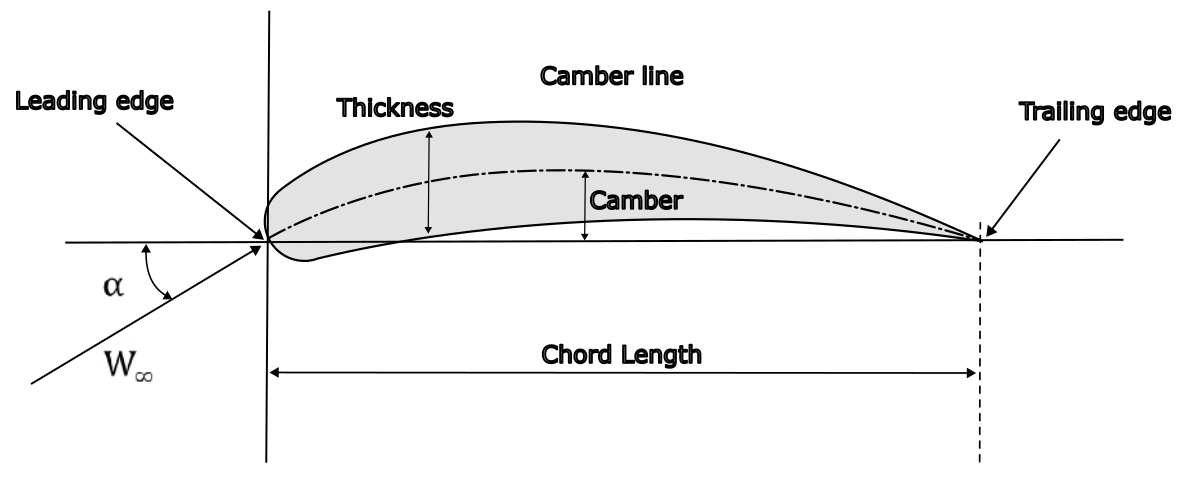
\includegraphics[width=0.8\linewidth]{Figures/Foil2d/Airfoil_basics.png}
    \caption{NACA\,00xx geometrical parameters used throughout the present work.}
    \label{fig:airfoil_geometry}
\end{figure}
 
Three families of two-dimensional coefficients describe the response of an airfoil section to a given relative flow. The lift coefficient $C_L$, the drag coefficient $C_D$ and the minimum-pressure coefficient $C_{p,\min}$ are non-dimensional forms of, respectively, the lift force per unit span, the drag force per unit span, and the lowest static pressure recorded on the section surface. They are defined as
\begin{equation}
C_L \;=\; \frac{L'}{\tfrac{1}{2}\rho V_\infty^{2} c}, \qquad
C_D \;=\; \frac{D'}{\tfrac{1}{2}\rho V_\infty^{2} c}, \qquad
C_{p,\min} \;=\; \frac{p_{\min} - p_\infty}{\tfrac{1}{2}\rho V_\infty^{2}},
\label{eq:CL_CD_Cpmin}
\end{equation}
with $V_\infty$ the freestream relative velocity, $\rho$ the fluid density, $c$ the chord, and $p_\infty$ the freestream static pressure. In a stator cascade these coefficients are reported per radial section and are functions of incidence, geometry and Reynolds number~\cite{Abbott1959}.
 
In the present application, NACA-type symmetric profiles with prescribed thickness ratio and rounded leading edges are used as a base, and the camber line is constructed to match the desired metal angles $\theta_1(r)$ and $\theta_2(r)$ along the span. The link between flow angle, loading and losses is established through the slip-correction methodology established in the project work~\cite{Leonsen2025} and through the cascade analysis developed in Section~\ref{sec:theory_cascade}. The detailed geometric construction implemented in the parametric MATLAB tool used for this thesis is described in Section~\ref{sec:theory_geometric_construction}.
 
% ---------------------------------------------------------------------
\section{Swirl metrics and critical phenomena}
\label{sec:theory_swirl_metrics_def}
 
Quantification of the swirling motion downstream of the RDT and downstream of the guide vanes is one of the central tasks of the post-processing in this thesis. The key quantity is the non-dimensional swirl number $S$. A standard definition expresses it as the ratio between the axial flux of angular momentum and the axial flux of axial momentum times a characteristic radius~\cite{Gupta1984, Vignat2022}:
\begin{equation}
S(z) \;=\; \frac{1}{R}\,\frac{G_\theta(z)}{G_z(z)},
\label{eq:S_def}
\end{equation}
where for an axisymmetric duct of radius $R$
\begin{align}
G_\theta(z) \;&=\; 2\pi\!\int_0^R \rho\, r^2 \, U_\theta(r,z)\,U_z(r,z)\,\mathrm{d}r,
\label{eq:Gtheta}\\
G_z(z) \;&=\; 2\pi\!\int_0^R \rho\, r \, U_z^{2}(r,z)\,\mathrm{d}r.
\label{eq:Gz}
\end{align}
The fundamental design objective of the guide vanes is to reduce $S(z)$ from the high values established by the RDT towards values close to zero at the RPT inlet. The post-processing in this thesis evaluates $S$ at every analysis plane in the domain (Section~\ref{sec:methods_planes_metrics}). This tracks the spatial development of the swirl along the entire path from the RDT through the bend to the RPT inlet.
 
\paragraph{Alternative swirl-number definitions.}
Equation~\ref{eq:S_def} is the form most often used in the combustion literature and is the form adopted as the primary metric in this thesis. However, the swirl number is not unique. Vignat et al.~\cite{Vignat2022} show that, when applied to non-uniform velocity profiles or in the presence of significant pressure terms, several formally equivalent definitions can give numerical values that differ by tens of percent. Two variants are particularly relevant here. The \emph{angle-based} swirl indicator
\begin{equation}
\overline{\alpha}(z) \;=\; \arctan\!\Bigl(\overline{U_\theta}^{\,m}(z)/\overline{U_z}^{\,m}(z)\Bigr)
\label{eq:alpha_bar}
\end{equation}
uses the mass-flow-averaged tangential and axial velocity components and has the advantage of being directly interpretable as a flow angle. The \emph{local swirling-strength} indicator $\lambda_{ci}$ identifies vortex cores from the imaginary part of the eigenvalues of the local velocity-gradient tensor and is the field used in CFX as \texttt{Velocity.Swirling Strength}. These two complement Eq.~\ref{eq:S_def}: $\overline{\alpha}$ summarises the bulk swirl orientation, $\lambda_{ci}$ is needed to identify discrete vortex structures such as tip vortices or precessing cores, and $S$ measures the total angular-momentum content of the cross-section. Reporting all three reduces the risk that a particular ranking depends on a particular definition.
 
\paragraph{Critical swirl and vortex breakdown.}
When the swirl ratio exceeds a critical value, swirling pipe flow can develop stagnation zones, wall separation and vortex breakdown~\cite{Rusak2014}. Critical $S$ values reported in the literature cluster around 0.6 for free swirling flows but depend on the specific definition and on the boundary conditions; in confined pipe flow with finite walls the threshold can be higher~\cite{Rusak2014}. Vortex breakdown is associated with large losses and strong unsteadiness, and it is the underlying mechanism behind the rotating vortex rope (RVR) in Francis-turbine draft tubes at off-design~\cite{Brekke2010}. In the present application, a residual $S(z)$ at the RPT inlet plane that is large enough to support breakdown would be unacceptable. The screening therefore checks the residual $S$ values against this threshold.
 
\subsection{Swirl decay in straight pipes}
\label{sec:theory_swirl_decay}
 
In a straight pipe with no swirl-conditioning element, the swirl decays through wall shear and turbulent transport. Experiments by Kitoh~\cite{Kitoh1991} and others show that the decay is approximately exponential and slow relative to typical duct lengths in industrial layouts:
\begin{equation}
S(z) \;\approx\; S(z_0)\,\exp\!\left[\,-\beta\,\frac{z - z_0}{D}\,\right],
\label{eq:S_decay}
\end{equation}
where the decay constant $\beta$ depends weakly on swirl level and Reynolds number and typically takes values $\beta \approx 0.02$-$0.06$ for smooth-walled turbulent flow~\cite{Kitoh1991, Beaubert2016}. The implication is that, for a duct length of a few diameters between the RDT and the RPT, the natural decay alone reduces $S$ only modestly. The decay also adds wall friction, so even the apparent ``benefit'' of letting the swirl decay over a long distance is partly cancelled by additional pressure loss compared with a non-swirling flow at the same Reynolds number. This is why an active swirl-recovery element close to the RDT is preferred over a long downstream pipe as passive damper~\cite{Andersen2014, Nguyen2024}.
 
\paragraph{Implication for the present geometry.}
In the present geometry, the path from the guide-vane trailing-edge plane to the RPT inlet has three sections: a conical contraction of about $0.50$~m, a $90^\circ$ bend, and about $1.0$~m of straight pipe in the final inlet section. This is short compared to the decay length expected from Eq.~\ref{eq:S_decay} for the swirl numbers seen at the guide-vane trailing edge. The residual swirl at the RPT inlet is therefore controlled almost entirely by what the guide vanes deliver and not by free decay in the pipe sections. The post-processing in this thesis quantifies this directly by comparing $S$ at the guide-vane trailing edge with $S$ at the bend exit and at the final inlet plane.
 
% ---------------------------------------------------------------------
\section{Cavitation considerations}
\label{sec:theory_cavitation}
 
Cavitation occurs when the local static pressure $p$ in the water falls to or below the vapour pressure $p_v$. Vapour bubbles form in low-pressure regions and collapse again when convected into higher-pressure regions, which can cause erosion, noise, vibration and loss of head and efficiency \cite{Gulich2010,Plesset1949}. An example of bubble growth and collapse near a wall is shown in Figure~\ref{fig:cavitation_bubbles}.
 
\begin{figure}[h!]
  \centering
  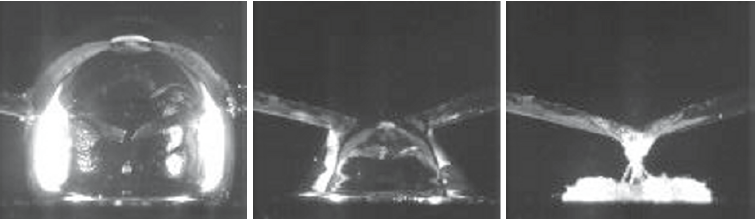
\includegraphics[width=0.8\textwidth]{Figures/Theory/Cavitation_bubbles.png}
  \caption[Cavitation bubbles]{Typical stages of cavitation bubble growth and collapse near a wall, adapted from G\"ulich~\cite{Gulich2010}.}
  \label{fig:cavitation_bubbles}
\end{figure}
 
In pump and pump-turbine applications, the cavitation risk is usually expressed through the available net positive suction head,
\begin{equation}
\mathrm{NPSH}_\mathrm{A} \;=\; \frac{p_{\mathrm{in}} - p_v}{\rho g},
\label{eq:npsha}
\end{equation}
where $p_{\mathrm{in}}$ is the absolute pressure at the machine inlet. For comparison with the machine head $H$, the Thoma cavitation number is
\begin{equation}
\sigma \;=\; \frac{\mathrm{NPSH}_\mathrm{A}}{H} \;=\; \frac{p_{\mathrm{in}} - p_v}{\rho g H},
\label{eq:sigma_thoma}
\end{equation}
and high $\sigma$ corresponds to safe operation, while low $\sigma$ is associated with bubble growth, head loss, efficiency loss and possible erosion~\cite{Franc2007, Gulich2010}.
 
For the NTNU RPT, Kerlefsen reports a required NPSH of approximately $1.3$-$1.4$~m for a net head $H_{\mathrm{net}} \approx 12$~m, giving $\mathrm{NPSH}_\mathrm{R}/H_{\mathrm{net}} \approx 0.11$-$0.12$, with a recommended margin of $20$-$25\,\%$ between available and required NPSH~\cite{Kerlefsen2025}. The Store2Hydro booster is intended to add approximately $H \approx 5$~m of head upstream of the RPT, which is comfortable as long as guide-vane losses are kept moderate. Any total-pressure loss in the screening therefore reduces the cavitation margin and is charged against the design.
 
In CFD, cavitation is commonly modelled as a homogeneous mixture of liquid water and water vapour, with mass-transfer rates determined by a Rayleigh-Plesset-based source term. In the present work no cavitation modelling is performed in the screening campaign; the static pressure field is examined for the absence of regions with $p < p_v$, but multiphase modelling is left as future work for the selected configuration.
 
% ---------------------------------------------------------------------
\section{Design requirements for the guide vanes}
\label{sec:theory_srv_requirements}
 
Figure~\ref{fig:rdt_streamlines} shows example streamlines downstream of the RDT from the design used in the present thesis. The design of the RDT is taken from Djupeslands work \cite{DjupeslandTrivedi2025}. The flow exhibits a strongly swirling wake with primary and secondary streamlines merging in vortex interactions across the cross-section.
 
\begin{figure}[h!]
  \centering
  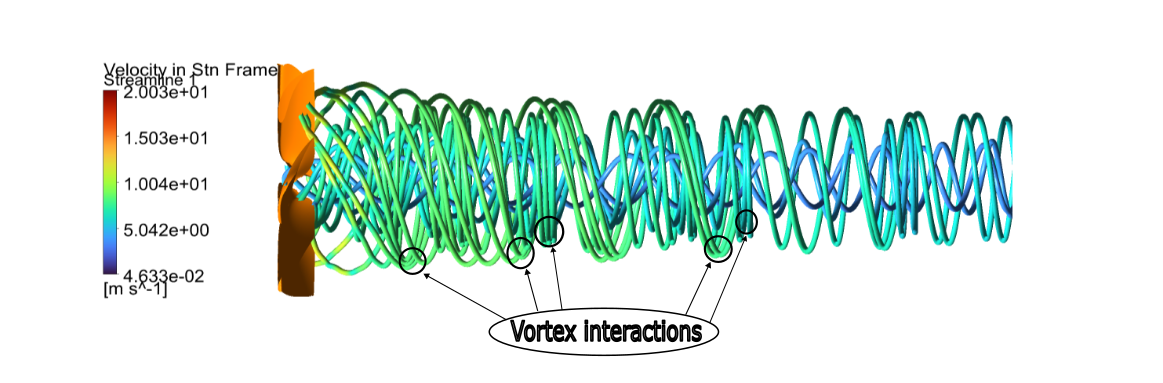
\includegraphics[width=0.99\textwidth]{Figures/Theory/Streamlines_shubham_Ink.png}
  \caption[Streamlines downstream of the RDT]{Streamlines downstream of the RDT from the design of Djupesland and Trivedi~\cite{DjupeslandTrivedi2025}. Primary and secondary streamlines merge in vortex interactions across the wake.}
  \label{fig:rdt_streamlines}
\end{figure}
 
The simulation also indicates very large local flow angles in the outer part of the wake. At $r \approx 0.25$~m, the absolute angle between $C_m$ and $C_u$ approaches $80^\circ$-$89^\circ$, meaning the velocity is almost entirely tangential. The guide vanes must therefore be designed to handle extreme inflow angles while still providing controlled turning and acceptable losses.
 
\subsection{Backflow region and the design span}
\label{sec:theory_backflow_span}
 
The RDT wake has a low-momentum or back-flow region in the centre. Post-processing of the RDT simulation~\cite{DjupeslandTrivedi2025} indicates that radii up to approximately $r \approx 0.144$~m experience back-flow, with $C_m < 0$ in this region (Figure~\ref{fig:UxUt}). The guide-vane design cannot adapt to this region because the flow direction is reversed and the vane has no inlet flow with positive momentum to operate on. The guide vanes are therefore designed as a hubless cascade, with the design span restricted to radii with positive meridional flow. In the present geometry this corresponds approximately to $r \in [0.12, 0.25]$~m, i.e.\ $r/R \in [0.48, 1.00]$. The associated flow-angle profile (Figure~\ref{fig:AngleRadius}) varies from approximately $89^\circ$ at the inner design radius to a minimum of about $60^\circ$ at $r \approx 0.225$~m, before increasing slightly again towards the shroud.
 
\begin{figure}[h!]
    \centering
    \includesvg[width=0.75\textwidth]{Figures/SVG/Ux_Ut.svg}
    \caption[Axial and tangential velocity profiles]{Axial and tangential velocity profiles versus radius, $0.25$~m downstream of the RDT~\cite{DjupeslandTrivedi2025}.}
    \label{fig:UxUt}
\end{figure}
\begin{figure}[h!]
    \centering
    \includesvg[width=0.75\textwidth]{Figures/SVG/Angle_radius.svg}
    \caption[Flow-field angle]{Flow-field angle versus radius, $0.25$~m downstream of the RDT~\cite{DjupeslandTrivedi2025}.}
    \label{fig:AngleRadius}
\end{figure}
 
The assumption is that the central recirculation zone carries low momentum flux compared with the main flow at larger radii and will partially mix out downstream before reaching the RPT runner. This assumption is examined in Chapter~\ref{chap:results_discussion} by comparing the central-region velocity field at the guide-vane outlet plane and at the bend exit.
 
\subsection{Tip-vortex mechanisms}
\label{sec:theory_tip_vortex}
 
When the inflow to the guide vanes has very high swirl, some streamlines hit the leading edge at angles so large that they cannot follow the geometry of the vane. Part of the flow then leaks around the inner free end of the vane into the hubless central region. The pressure difference between the pressure side and the suction side drives this tip-leakage flow, which rolls up into a tip-clearance vortex and creates extra induced vortices in the passage~\cite{You2007}. In the circular hubless cascade considered here, the same type of vortex can appear near the inner ends of the vanes even though the geometry is not a planar two-dimensional cascade. Figure~\ref{fig:Tip_vortex} sketches this mechanism. In the post-processing, this is the structure that the swirling-strength field $\lambda_{ci}$ should pick up most clearly near the inner span of the vanes.
 
\begin{figure}[h!]
  \centering
  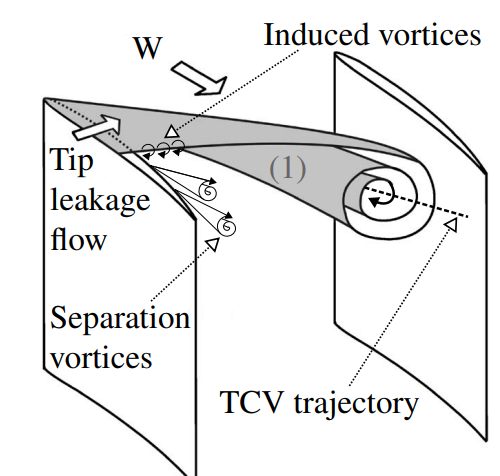
\includegraphics[width=0.40\textwidth]{Figures/Theory/Tip_vortex}
  \caption[Tip-leakage vortex mechanism]{Schematic of tip-leakage flow and the formation of a tip-clearance vortex (TCV), adapted from You et al.~\cite{You2007}.}
  \label{fig:Tip_vortex}
\end{figure}
 
% ---------------------------------------------------------------------
\section{Cascade theory for guide vanes}
\label{sec:theory_cascade}
 
\subsection{Solidity and pitch}
\label{sec:theory_solidity}
 
At each radius $r$, the guide vanes form an axial cascade with pitch
\begin{equation}
s(r) \;=\; \frac{2\pi r}{Z_s},
\label{eq:pitch}
\end{equation}
and local solidity
\begin{equation}
\sigma(r) \;=\; \frac{c(r)}{s(r)},
\label{eq:solidity}
\end{equation}
where $Z_s$ is the vane count and $c(r)$ is the local chord. Solidity controls how much turning the cascade can deliver; high solidity gives more turning per pitch but also more wetted surface, more friction loss and a higher risk of separation between adjacent vanes. The pitch and solidity for the present geometry, evaluated for a fixed chord $c = 0.25$~m and the vane counts $Z_s \in \{6, 8, 9\}$ used in the screening matrix, are summarised in Table~\ref{tab:pitch_solidity_design}. The table illustrates a recurring feature of hubless designs: the local solidity rises sharply at the inner radius because the pitch shrinks with $r$, so even a moderate global vane count produces a heavily loaded inner span.
 
\begin{table}[h!]
\centering
\caption[Pitch and solidity for selected vane counts]{Pitch $s(r)$ and solidity $\sigma(r)$ for guide vanes with chord $c = 0.25$~m in a pipe of diameter $D = 0.5$~m, for the vane counts $Z_s \in \{6,8,9\}$ used in the screening matrix and $r \in [0.12, 0.25]$~m.}
\label{tab:pitch_solidity_design}
\small
\begin{tabular}{c|cc|cc|cc}
\toprule
\textbf{$r$ (m)} & $s$ ($Z{=}6$) & $\sigma$ & $s$ ($Z{=}8$) & $\sigma$ & $s$ ($Z{=}9$) & $\sigma$ \\
\midrule
0.12 & 0.1257 & 1.99 & 0.0942 & 2.65 & 0.0838 & 2.98 \\
0.15 & 0.1571 & 1.59 & 0.1178 & 2.12 & 0.1047 & 2.39 \\
0.18 & 0.1885 & 1.33 & 0.1414 & 1.77 & 0.1257 & 1.99 \\
0.21 & 0.2199 & 1.14 & 0.1649 & 1.52 & 0.1466 & 1.71 \\
0.25 & 0.2618 & 0.95 & 0.1963 & 1.27 & 0.1745 & 1.43 \\
\bottomrule
\end{tabular}
\end{table}
 
\subsection{Diffusion factor and the de Haller criterion}
\label{sec:theory_diffusion}
 
A standard measure of how heavily a blade row is loaded is the Lieblein diffusion factor~\cite{Lieblein1953}:
\begin{equation}
D_f \;=\; 1 - \frac{V_{\mathrm{out}}}{V_{\mathrm{in}}}
       + \frac{\lvert V_{\theta,\mathrm{out}} - V_{\theta,\mathrm{in}} \rvert}
              {2\,\sigma\, V_{\mathrm{in}}},
\label{eq:Df}
\end{equation}
with $V_{\mathrm{in}}$, $V_{\mathrm{out}}$ the inlet and outlet relative velocities, $V_{\theta,\mathrm{in}}$, $V_{\theta,\mathrm{out}}$ the corresponding tangential components, and $\sigma$ the local solidity. Lieblein recommends $D_f \lesssim 0.6$ to keep the suction-side boundary layer attached. A complementary screening criterion is the de Haller bound on the relative-velocity ratio,
\begin{equation}
\frac{V_{\mathrm{out}}}{V_{\mathrm{in}}} \;\geq\; 0.72,
\label{eq:deHaller}
\end{equation}
which is independent of solidity but cruder than $D_f$. Both criteria are used in the post-processing as descriptive indicators rather than as binary go/no-go limits, because the present application requires turning angles up to $80^\circ$-$90^\circ$ that are well beyond the conventional axial-compressor regime.
 
\subsection{Incidence, deviation and effective turning}
\label{sec:theory_incidence_deviation}
 
Section~\ref{sec:theory_kinematics} introduced the inlet and outlet flow angles $\beta_1(r)$ and $\beta_2(r)$, the metal angles $\theta_1(r)$ and $\theta_2(r)$, the incidence $i(r)$, and the deviation (slip) angle $\delta(r)$. In the cascade view these quantities are used as design constraints:
\begin{itemize}
  \item the leading edge should see a small incidence $i(r)$ at the design point, to avoid early separation and additional loss;
  \item the deviation $\delta(r)$ determines how much of the geometric turning $\theta_1 - \theta_2$ actually appears as flow turning $\beta_1 - \beta_2$;
  \item the effective turning is therefore smaller than the geometric turning, especially for low solidity and high loading.
\end{itemize}
The deviation is treated as a fixed correction $\delta_{\mathrm{TE}} = 6^\circ$ added to the trailing-edge metal angle, following G\"ulich~\cite{Gulich2010}. The project-work response surface~\cite{Leonsen2025} predicts $10^\circ$-$20^\circ$ at the high turning required here. Adopting those values would aggressively over-camber the trailing edge, sharpen the suction-side pressure gradient, and promote separation. The fixed $6^\circ$ correction captures the bulk of the deviation effect without overloading the cascade.

The cost of this choice is that the screening reports the swirl-reduction performance achievable with a conservative slip correction, not the maximum achievable performance. This choice is revisited in Chapter~\ref{chap:results_discussion} when the swirl-reduction results are interpreted.
 
% ---------------------------------------------------------------------
\section{Geometric construction of the guide vanes}
\label{sec:theory_geometric_construction}
 
This section describes the geometric construction of each two-dimensional vane section that is produced by the parametric MATLAB tool \texttt{vanedesign\_loft\_export}. The presentation is organised so that each step in the construction can be related to a specific design parameter exposed in the run script \texttt{run\_file\_GV\_DESIGN.m}, which supports later interpretation of the simulation results.
 
\subsection{Chordwise coordinate and clustering}
\label{sec:theory_clustering}
 
A non-dimensional chordwise coordinate $x^* = x/c \in [0, 1]$ is used with cosine clustering near the leading and trailing edges,
\begin{equation}
x^* \;=\; \frac{1 - \cos(\pi t)}{2}, \qquad t \in [0, 1],
\label{eq:cosine_clustering}
\end{equation}
which concentrates points where the surface curvature and the pressure gradient are largest. Cosine clustering is standard practice in airfoil design because it reduces geometric truncation errors at the leading and trailing edges and is preserved when the section is wrapped on a cylindrical or conical surface.
 
\subsection{Cubic camber line and metal-angle matching}
\label{sec:theory_camber}
 
The camber line is a cubic polynomial in $x^*$,
\begin{equation}
\frac{y_c(x^*)}{c} \;=\; A x^{*3} + B x^{*2} + C x^*,
\label{eq:camber_cubic}
\end{equation}
The coefficients $A$, $B$, $C$ are chosen to match two slope conditions in a frame aligned with the stagger angle $\zeta$. At $x^* = 0$ the local slope of $y_c$ matches the LE metal angle $\theta_1$, and at $x^* = 1$ it matches the TE metal angle $\theta_2$. The cubic form has three free coefficients, which is sufficient to enforce the two slope conditions and one normalisation condition. A cubic polynomial is preferred over a parabola or a circular arc because it allows the LE and TE slopes to be specified independently, which is necessary to match arbitrary inflow and target outflow angles. The choice ties the camber directly to the velocity-triangle requirement and is the reason the design tool can be driven from spanwise inlet data $r$, $C_m(r)$, $C_u(r)$.
 
\subsection{Modified NACA 00xx thickness law}
\label{sec:theory_thickness}
 
The thickness law follows the classical NACA 00-series formula~\cite{Abbott1959}:
\begin{equation}
\frac{t_{\mathrm{base}}(x^*)}{c} \;=\; 5\!\left(0.2969\sqrt{x^*} - 0.1260\,x^* - 0.3516\,x^{*2} + 0.2843\,x^{*3} - 0.1015\,x^{*4}\right),
\label{eq:naca_thickness}
\end{equation}
which produces a symmetric profile with maximum thickness near $x^* \approx 0.30$. Two modifications adapt the law to the guide-vane application. A leading-edge roundness factor $\texttt{LE\_round}$ adjusts the thickness near $x^* = 0$ as
\begin{equation}
t_{\mathrm{LE}}(x^*) \;=\; t_{\mathrm{base}}(x^*)\,\Bigl[\,1 + (\texttt{LE\_round}-1)\,(1-x^*)^2\,\Bigr],
\label{eq:LE_round}
\end{equation}
which thickens the leading edge for $\texttt{LE\_round} > 1$ and thereby reduces sensitivity to off-design incidence. A finite trailing-edge thickness ratio $t_{\mathrm{TE,rel}}$ is added linearly, $t(x^*)/c = a\,t_{\mathrm{LE}}(x^*) + t_{\mathrm{TE,rel}}\,x^*$, with the scale factor $a$ chosen so that $\max_x t(x^*)/c$ matches a prescribed target $(t/c)_{\mathrm{rel}}$. Throughout the present work, $(t/c)_{\mathrm{rel}} = 0.075$ and $\texttt{LE\_round} = 1.2$ are kept fixed, in line with the project work~\cite{Leonsen2025}.
 
\subsection{Stagger angle, lean and sweep}
\label{sec:theory_stagger_lean_sweep}
 
The stagger angle $\zeta(r)$ orients the chord line relative to the axial direction. It is determined by the choice of metal angles $\theta_1(r)$ and $\theta_2(r)$ together with the geometric definition that places the chord line at the average of the LE and TE positions in the rotated frame. In addition to the stagger, the design tool exposes two spanwise stacking parameters: \emph{lean} $\texttt{lean\_amp}$ tilts the section in the tangential direction along the span, and \emph{sweep} $\texttt{sweep\_amp}$ shifts the section in the axial direction along the span. Lean and sweep are used in modern axial design to control radial pressure gradients and mitigate secondary flows~\cite{Schnoes2018}. In the screening campaign of this thesis they are held at zero, so the chord and solidity factors can be isolated. Lean and sweep are listed as candidates for a second-stage refinement campaign in Chapter~\ref{chap:future_work}.
 
\subsection{Cylindrical or conical wrapping}
\label{sec:theory_wrapping}
 
The two-dimensional sections are stacked along the span and wrapped on either a cylindrical surface of radius $r$ or a conical surface with radius varying linearly with the axial coordinate~\cite{Leonsen2025}. The azimuthal coordinate of each section point is computed from the tangential coordinate and a global trailing-edge anchoring angle. The trailing edges of all sections can be anchored to a common azimuth, $\phi_{\mathrm{TE,global}}$, which produces a straight TE line in the axial-azimuthal plane and supports a clean axial through-flow when the residual swirl is small. In the present work, cylindrical wrapping is used because the guide-vane domain has constant duct diameter and there is no need to wrap on a cone. The TE-anchored option is enabled, which produces all sections aligned at the same azimuth at the trailing edge.
 
\subsection{Constant chord versus constant solidity}
\label{sec:theory_const_chord_const_sol}
 
The two design strategies adopted in the screening campaign are exposed by the boolean flag \texttt{use\_sigma} in the design tool:
\begin{itemize}
  \item \textbf{Constant chord (CC).} The chord $c$ is a single constant value, identical at every radius. The solidity $\sigma(r) = c\,Z_s/(2\pi r)$ then decreases hyperbolically with radius, so the loading per pitch is concentrated near the inner span and decreases towards the shroud.
  \item \textbf{Constant solidity (CS).} The chord is set as $c(r) = \sigma_{\mathrm{target}}\,s(r)$ with $\sigma_{\mathrm{target}}$ fixed, so the solidity is uniform in radius and the chord scales linearly with $r$. The loading is more even radially, but the wetted surface and the friction loss are larger because the outer span receives the longest chord.
\end{itemize}
The two strategies are not equivalent, and the screening campaign is constructed precisely to compare them at matched levels of loading. The case-naming convention used throughout this thesis is \texttt{<strategy>\_<chord>\_<Zs>}. For example, \texttt{CC\_400\_8} denotes a constant-chord design with $c = 400$~mm and $Z_s = 8$. \texttt{CS\_400\_8} denotes a constant-solidity design with the same shroud chord, but with chord scaling linearly inwards.

The geometric difference between the two strategies is illustrated in Figure~\ref{fig:cc_vs_cs_3d} for the matched pair \texttt{CC\_400\_8} and \texttt{CS\_400\_8}. Both designs share the same shroud chord ($c_{\mathrm{shroud}} = 400$~mm) and the same vane count ($Z_s = 8$). The CC vane keeps a constant chord all the way to the inner cut-out at $r = 0.12$~m. The CS vane tapers linearly inwards, so the chord at the hub is reduced to $c_{\mathrm{hub}} = \sigma_{\mathrm{shroud}}\,(2\pi r_{\mathrm{hub}}/Z_s) \approx 191$~mm. Three-dimensional renderings of all 18 active configurations are collected in Appendix~\ref{app:gv_3d_geometries}.

\begin{figure}[h!]
  \centering
  \begin{subfigure}[b]{0.48\textwidth}
    \centering
    \fbox{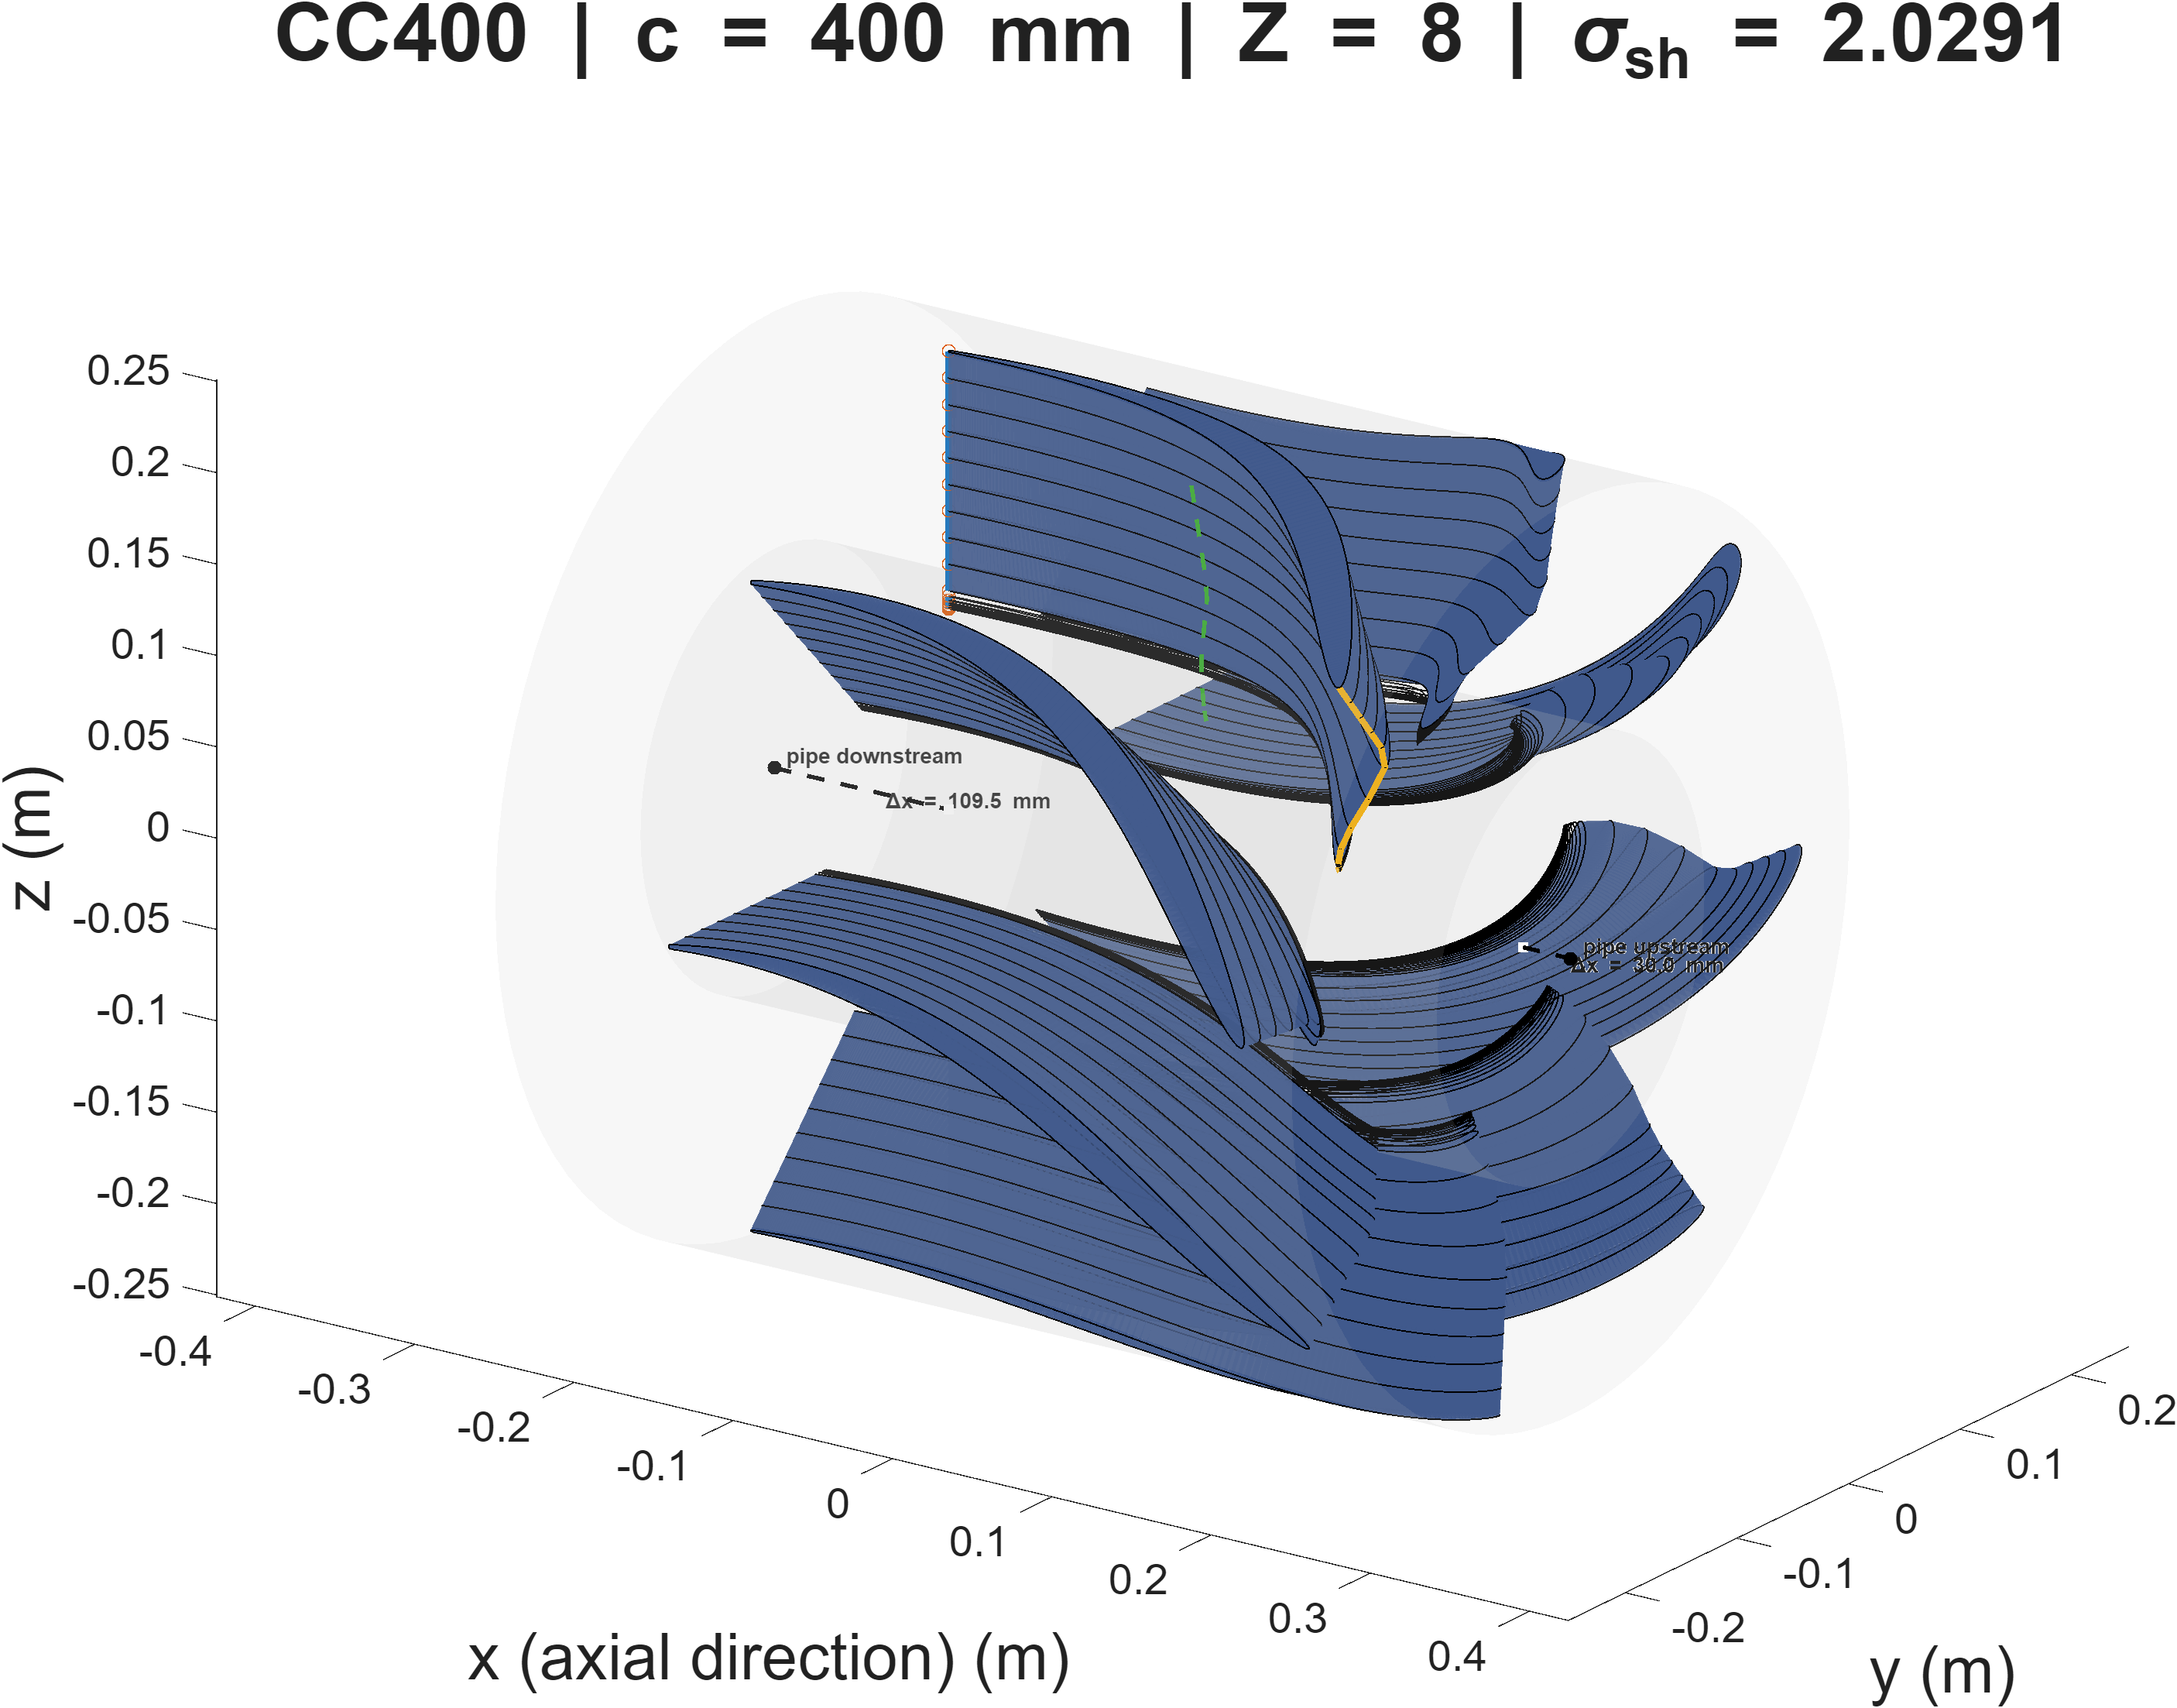
\includegraphics[width=\textwidth]{Figures/GV_Design/3D/CC_400_8_Helices_Vane_axial_X_.png}}
    \caption{\texttt{CC\_400\_8}: constant chord $c = 400$~mm at every radius. Solidity is highest at the hub and decreases towards the shroud.}
    \label{fig:cc_400_8_3d}
  \end{subfigure}
  \hfill
  \begin{subfigure}[b]{0.48\textwidth}
    \centering
    \fbox{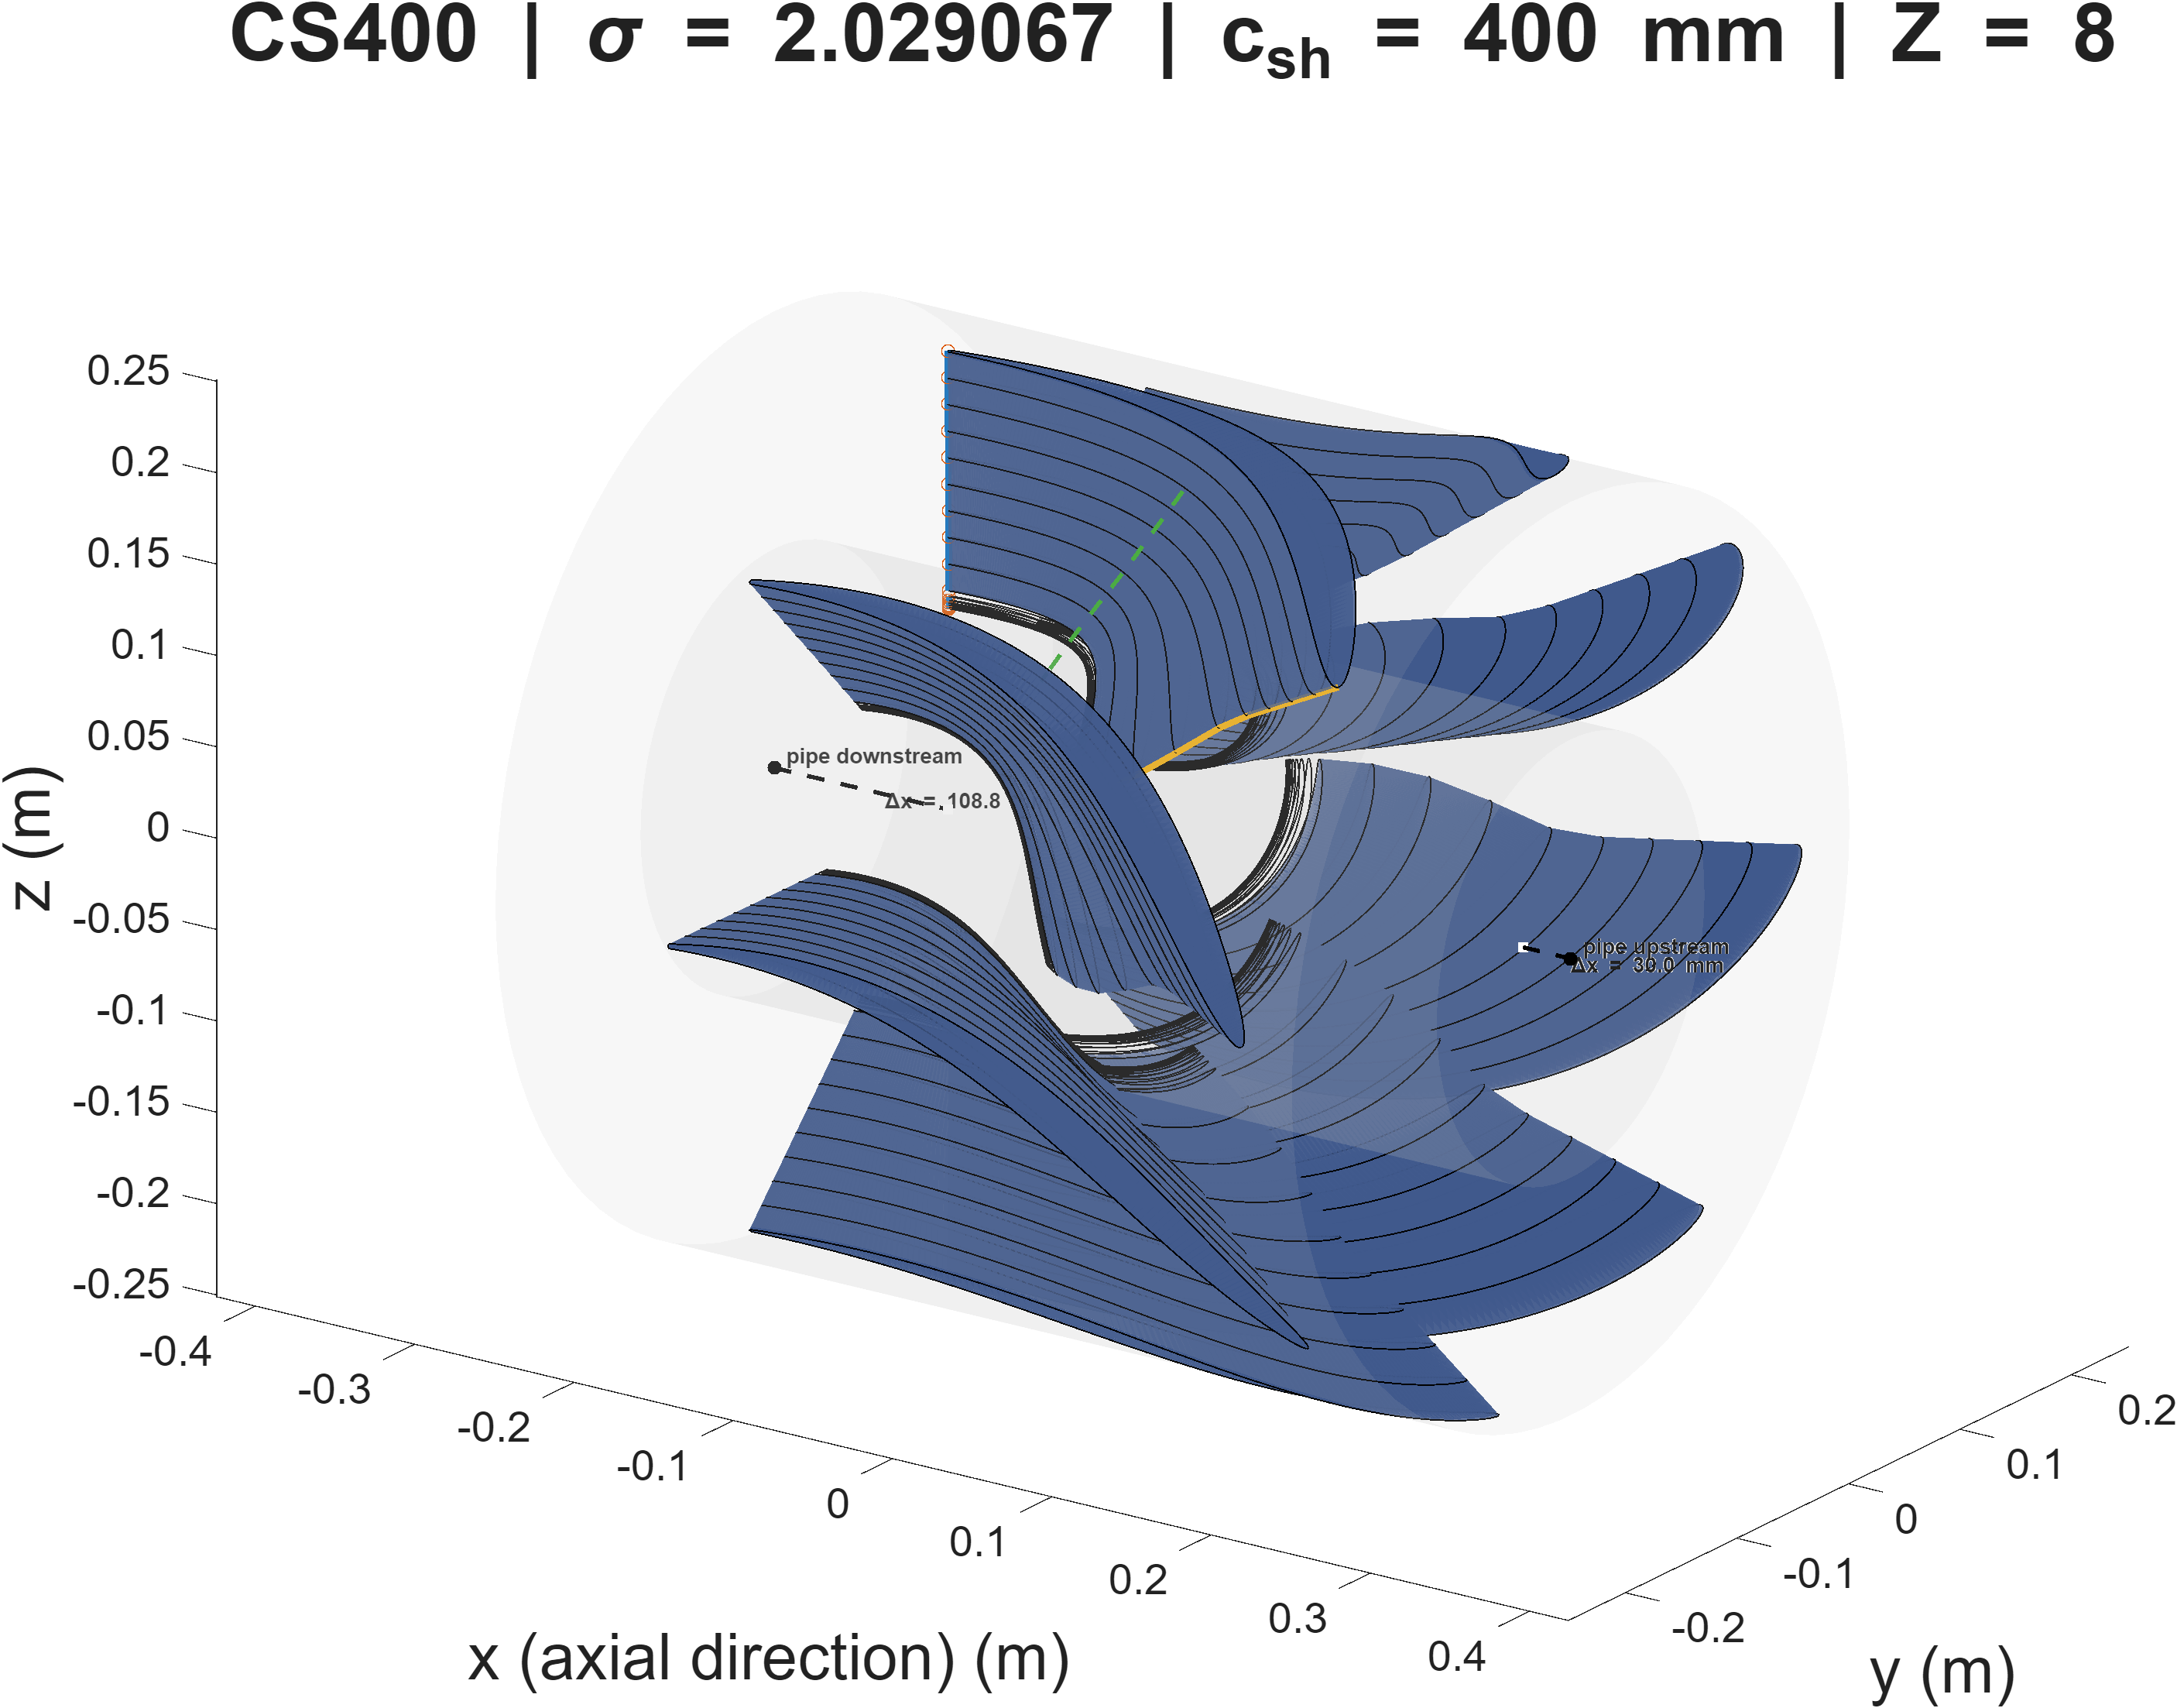
\includegraphics[width=\textwidth]{Figures/GV_Design/3D/CS_400_8_Helices_Vane_axial_X_.png}}
    \caption{\texttt{CS\_400\_8}: constant solidity referenced at the shroud. The chord is reduced linearly with $r$ from $c_{\mathrm{shroud}} = 400$~mm to $c_{\mathrm{hub}} \approx 191$~mm.}
    \label{fig:cs_400_8_3d}
  \end{subfigure}
  \caption[CC versus CS guide-vane geometries]{Three-dimensional rendering of the matched pair \texttt{CC\_400\_8} and \texttt{CS\_400\_8} ($c_{\mathrm{shroud}} = 400$~mm, $Z_s = 8$). Both designs share the same shroud chord; only the radial chord distribution differs. Renderings of all 18 active configurations are given in Appendix~\ref{app:gv_3d_geometries}.}
  \label{fig:cc_vs_cs_3d}
\end{figure}
 
% ---------------------------------------------------------------------
\section{Secondary flow and Dean vortices in 90$^\circ$ bends}
\label{sec:theory_dean_bend}
 
The geometry adopted for the screening campaign includes a $90^\circ$ bend between the cone and the final inlet section. This element is not passive. When fluid passes through a curved duct, the centripetal acceleration $V^2/R_c$ requires a radial pressure gradient across the cross-section. The velocity, however, is not uniform: it is reduced near the wall by the boundary layer and is largest in the core of the duct. The local centripetal acceleration is therefore not uniform across the section, and the cross-stream pressure gradient cannot balance it everywhere simultaneously. The fluid responds by establishing a pair of counter-rotating secondary cells in the cross-stream plane: the \emph{Dean vortices}~\cite{Dean1927}.
 
\subsection{The Dean number and bend regimes}
\label{sec:theory_dean_number}
 
The strength of the Dean vortices scales with the dimensionless Dean number
\begin{equation}
\mathrm{De} \;=\; \mathrm{Re}\,\sqrt{\frac{D_h}{2\,R_c}},
\label{eq:dean}
\end{equation}
where $D_h$ is the hydraulic diameter of the duct and $R_c$ is the radius of curvature of the bend centreline. For the present geometry the duct diameter at the bend is approximately $D = 0.4$~m and the bend curvature radius is on the order of $R_c \approx 0.3$-$0.4$~m. With Reynolds numbers around $\mathrm{Re} \sim 10^6$ in the duct, the Dean number is well into the turbulent regime where the Dean cells are fully developed and may further interact with the upstream-imposed swirl. Three regimes are commonly distinguished. For $\mathrm{De} \lesssim 100$, the bend secondary flow is laminar and weak. For intermediate Dean numbers, instabilities and additional secondary cells (D\"ottner cells) emerge. For high Reynolds numbers, the secondary motion is fully turbulent and is dominated by two large counter-rotating Dean cells, with additional small-scale features near the inner radius where separation is most likely.
 
\subsection{Interaction with upstream swirl}
\label{sec:theory_swirl_bend_interaction}
 
When the upstream flow already carries swirl, the Dean cells and the swirl interact, and the interaction depends on the sign of the swirl. If the upstream swirl rotates in the same sense as one of the two Dean cells, that cell is amplified and the opposite cell is suppressed; if the upstream swirl rotates in the opposite sense, the partition is reversed. The post-bend axial-velocity profile is therefore generally asymmetric in a way that depends on the \emph{sign} of the residual swirl, not only on its magnitude. Liu and Vanierschot~\cite{LiuVanierschot2021} review this regime and document that the asymmetry persists for several diameters downstream of the bend exit. Escue and Cui~\cite{EscueCui2010} demonstrate that the SST $k$-$\omega$ model captures the bulk structure of swirling pipe flow. The model tends to underpredict turbulence anisotropy under strong rotation, which is a recognised limitation when interpreting RANS results in this regime.
 
The implication for the present thesis is that:
\begin{enumerate}
  \item the guide-vane performance must be evaluated not only at the trailing-edge plane (where the design tool has direct geometric leverage) but also at planes downstream of the bend, because swirl-bend interaction changes the effective ranking;
  \item the sign of the residual swirl is a relevant design parameter even if the screening matrix focuses primarily on chord-strategy and vane count;
  \item asymmetry of the axial-velocity profile at the RPT inlet plane, not just its mean magnitude, must be reported.
\end{enumerate}
 
\subsection{Inner-radius separation in the bend}
\label{sec:theory_bend_separation}
 
A further bend-related effect is separation on the inner radius of the bend, where the adverse pressure gradient is strongest. Jenssen~\cite{Jenssen2020} reported this effect in the original RPT draft-tube geometry and used it to motivate the placement of a velocity-profile boundary condition downstream of the bend rather than upstream. In the present configuration the same inner-radius separation may occur and is likely to be more severe when the upstream swirl reinforces the inner-side pressure gradient. The screening campaign reports the static-pressure field along the bend centreline and the wall-streamline pattern on the inner radius for the shortlisted cases.
 
% ---------------------------------------------------------------------
\section{Turbulence modelling and numerical limitations}
\label{sec:theory_turbulence}
 
The simulations in this thesis use a Reynolds-averaged formulation with the SST $k$-$\omega$ turbulence model of Menter~\cite{Menter1994}. The SST model blends the standard $k$-$\omega$ model in the near-wall region, where it is robust under adverse pressure gradients, with a $k$-$\varepsilon$ formulation in the outer flow. It is the de-facto standard for hydraulic turbomachinery in industrial CFD and has been validated extensively in pump, turbine and stator applications. The known limitations relevant to the present work are summarised here and revisited where the corresponding limitation is in play.
 
\paragraph{Anisotropy under strong rotation.} Two-equation eddy-viscosity models assume an isotropic eddy viscosity and cannot represent the full Reynolds-stress anisotropy under strong rotation or strongly curved streamlines. In swirling pipe flow this leads to underprediction of secondary kinetic energy in the cross-stream plane and to a slightly diffused tangential-velocity profile compared with experimental data~\cite{EscueCui2010}.
 
\paragraph{Streamline curvature and bend secondary flow.} The Dean vortices in the $90^\circ$ bend are produced by the same streamline-curvature mechanism that two-equation eddy-viscosity models tend to underpredict. The bulk Dean structure is captured, but the magnitude of the secondary-velocity components and the location of inner-radius separation can be sensitive to mesh resolution and to the specific blending of the SST coefficients. The interpretation in Chapter~\ref{chap:results_discussion} is therefore qualitative when comparing absolute Dean strengths between configurations and quantitative when comparing relative changes between similar configurations.
 
\paragraph{Transition modelling.} Transition is not modelled in the SST formulation used here. The Reynolds numbers in the present application are large enough that the boundary layers on the guide vanes are turbulent everywhere. A small region close to the leading edge of the inner span, where the local chord-Reynolds number is lowest, may be the only exception. The expected effect of neglected transition is a small underestimation of leading-edge loss, which is the same direction for all configurations and therefore does not affect the comparative ranking.
 
\paragraph{Steady RANS for the screening.} The 18-case screening uses steady RANS. The inherent unsteadiness from rotor-stator interaction, from vortex shedding at the guide-vane trailing edge, and from any precessing vortex core developing downstream is therefore not resolved. Two separate transient simulations of selected configurations are performed to address the rotor-stator interaction question (Sections~\ref{sec:rsi-thesis}-\ref{sec:spec-coherence}). Full transient screening of all 18 configurations is not feasible within the time-frame and is left as future work.

% ---------------------------------------------------------------------
\section{Rotor-stator interaction and pressure pulsations}
\label{sec:rsi}
 
In the compact RDT-GV-duct configuration considered in this thesis, the rotating RDT blades and the stationary GV ring are separated by a relatively small axial distance. The flow through the GV is therefore not strictly steady, even at the nominal operating point. Two mechanisms produce unsteady loading on the GV and a corresponding pressure pulsation field in the duct~\cite{Brekke2015, Arndt1990}:
\begin{enumerate}
  \item \emph{Potential interaction.} The pressure field attached to each rotor blade convects past the stationary vanes. It produces a pressure fluctuation that decays exponentially with axial distance but can be significant when the axial gap is a fraction of a blade chord.
  \item \emph{Viscous (wake) interaction.} Each rotor blade sheds a velocity-deficit wake. When such a wake is chopped by a stationary vane, the local angle of attack changes momentarily and produces an impulsive change in vane loading.
\end{enumerate}
Both mechanisms are periodic in the rotor reference frame at the rotor frequency $f_n$, and in the stator reference frame at the blade passing frequency $f_{\mathrm{BPF}}$ defined below. They are the main source of deterministic unsteadiness in the present configuration.

\subsection{Axial spacing between the rotor and the stationary vane row}
\label{sec:rsi-axial-spacing}

Rotor-stator interaction strength scales with the axial distance between the rotor trailing edge and the stator leading edge. In compact axial-pump stages this clearance is non-dimensionalised by the impeller chord $L$ as $a/L$, with $a$ the axial gap. G\"ulich~\cite{Gulich2010} recommends a clearance in the range
\begin{equation}
    \frac{a}{L} \;=\; 0.05\,\text{-}\,0.15
    \label{eq:gulich_a_over_L}
\end{equation}
to limit dynamic vane loading and pressure pulsations from rotor-stator interaction. Bijukchhe and Trivedi~\cite{Bijukchhe2026} adopt the same range in their recent design study of axial booster pumps for retrofitted reversible pump-turbines. They add a further recommendation that the impeller-to-stator vane-count ratio satisfies $Z_r/Z_s \approx 0.7$-$0.9$, to weaken harmonic reinforcement at the rotor-stator interface. The ratios used in the screening matrix of this thesis are $Z_r/Z_s = 7/6 \approx 1.17$, $7/8 = 0.875$ and $7/9 \approx 0.78$. The $Z_s = 8$ and $Z_s = 9$ families fall inside or close to the recommended window. The $Z_s = 6$ family lies outside it.

The recommendation~\eqref{eq:gulich_a_over_L} was developed for compact axial-pump stages, in which the diffuser vanes are placed immediately downstream of the impeller. The geometry studied in this thesis differs from this configuration. The hubless RDT discharges into a duct section that connects to the guide-vane row, and the stationary vanes are not placed at the rotor trailing edge. The bound~\eqref{eq:gulich_a_over_L} is therefore retained as a qualitative reference for why the axial spacing matters, rather than as a binding design constraint. The actual axial spacing in the present geometry is documented in Section~\ref{sec:methods_axial_spacing}, and the practical implications for the rotor-stator interaction analysis are discussed in Section~\ref{sec:rsi-thesis} and revisited in the spectral analysis of Chapter~\ref{chap:results_discussion}.

\subsection{Rotor frequency and blade passing frequency}
\label{sec:rsi-bpf}
 
With rotor rotational speed $n$~(rpm), the rotor frequency is
\begin{equation}
    f_n \;=\; \frac{n}{60}. \label{eq:fn}
\end{equation}
A single stationary vane observes $Z_r$ rotor blades passing in each rotor revolution. The fundamental excitation frequency seen by a single GV is therefore the \emph{blade passing frequency}~\cite{Brekke2015}
\begin{equation}
    f_{\mathrm{BPF}} \;=\; Z_r\, f_n. \label{eq:fbpf}
\end{equation}
A single rotor blade sees $Z_s$ stationary vanes per rotor revolution and therefore experiences a periodic loading at the \emph{vane passing frequency}
\begin{equation}
    f_{\mathrm{VPF}} \;=\; Z_s\, f_n. \label{eq:fvpf}
\end{equation}
In the special case $Z_r = Z_s$ the two frequencies coincide, $f_{\mathrm{BPF}} = f_{\mathrm{VPF}}$. Higher harmonics $k f_{\mathrm{BPF}}$, $k=2,3,\dots$ are typically present because the actual pulse shape is not sinusoidal; their amplitude decreases with $k$ but can remain non-negligible for the second and third harmonic if the wake is narrow~\cite{Egusquiza2006,Rodriguez2007}.
 
\subsection{Tyler-Sofrin modal decomposition}
\label{sec:rsi-tyler}
 
The classical analysis by Tyler and Sofrin~\cite{Tyler1962} for an annular rotor-stator stage shows that the unsteady pressure field downstream of the stator can be written as a sum of circumferential modes
\begin{equation}
    p'(r,\theta,z,t) \;=\; \sum_{k=1}^{\infty}\sum_{j=-\infty}^{\infty}
      \hat{p}_{k,j}(r,z)\,
      \exp\!\left[\, i\bigl(m_{k,j}\,\theta - k\,Z_r\,\Omega\,t\bigr)\,\right],
    \label{eq:tyler_sofrin_expansion}
\end{equation}
where $\Omega = 2\pi f_n$ and the circumferential mode order is
\begin{equation}
    m_{k,j} \;=\; k\,Z_r - j\,Z_s, \qquad k,j \in \mathbb{Z}.
    \label{eq:tyler_sofrin}
\end{equation}
Each combination $(k,j)$ corresponds to a pressure pattern that rotates around the axis with phase speed $k\,Z_r\,\Omega/m_{k,j}$ and oscillates at frequency $k f_{\mathrm{BPF}}$ at a fixed point in the stator frame. The mode order $m_{k,j}$ determines how the pulsation couples with the surrounding duct: an $m=0$ pattern is axisymmetric and propagates as a plane wave, whereas patterns with $|m|\geq 1$ are spinning modes whose upstream or downstream propagation depends on whether the frequency is above or below the cut-off frequency of the corresponding duct mode~\cite{Morse1968}.
 
For the fundamental BPF harmonic $k=1$ the lowest-order spatial mode is
\begin{equation}
    m_{\min} \;=\; \min_{j\in\mathbb{Z}} \bigl| Z_r - j\,Z_s \bigr|.
    \label{eq:mmin}
\end{equation}
Three cases are of particular relevance:
\begin{itemize}
  \item If $Z_r = Z_s$, Eq.~\eqref{eq:mmin} gives $m_{\min}=0$ with $k=j=1$. The lowest-order mode at $f_{\mathrm{BPF}}$ is the \emph{axisymmetric breathing mode}: all $Z_s$ vanes are loaded synchronously and in phase. The pressure field is a plane wave that propagates along the duct without a cut-off, and the integrated axial force on the GV ring adds coherently at $f_{\mathrm{BPF}}$.
  \item If $\gcd(Z_r,Z_s)=1$ (coprime), the minimum mode order is at least $|Z_r - Z_s|$ and typically $m_{\min} \geq 1$. The net axial force on the ring approaches zero by cancellation around the circumference. The remaining loading appears as a rotating radial force on the rotor.
  \item If $Z_r = Z_s = 7$, which corresponds to the configuration most directly inherited from the project work and which forms one of the two transient baselines analysed in this thesis, the breathing mode $m=0$ is unavoidable in principle. Whether it actually dominates the pulsation field in practice depends on how closely the true wake pattern of the RDT satisfies the $Z_r$-fold azimuthal symmetry that the Tyler-Sofrin argument assumes.
\end{itemize}
It is therefore an established design guideline in axial turbomachinery to choose $Z_r$ and $Z_s$ such that low-order spatial modes are avoided at the harmonics of concern, especially when structural or acoustic natural frequencies lie close to $f_{\mathrm{BPF}}$~\cite{Brekke2015,Egusquiza2006,Tanaka2011}. For reversible pump-turbines in particular, reference~\cite{Nduwayezu2021} reports that the vaneless-space pressure pulsation amplitude depends explicitly on the runner blade number, which supports treating $Z_s$ as a system-level design variable and not only as a hydraulic one.
 
\subsection{Structural and acoustic resonance}
\label{sec:rsi-resonance}
 
Unsteady blade forcing becomes critical when an excitation frequency in Eq.~\eqref{eq:tyler_sofrin_expansion} approaches a structural or acoustic natural frequency of the system. Two coupling categories are typically considered~\cite{Egusquiza2006,Tanaka2011}.
 
\paragraph{Structural resonance.} The GV blade, the GV ring, the RDT blades and the supporting structure each possess a discrete set of natural frequencies $\{f_k^s\}$. A resonance condition occurs when an excitation frequency $k\,f_{\mathrm{BPF}}$ or $k\,f_{\mathrm{VPF}}$ matches one of the $f_k^s$, \emph{and} the spatial mode order of the excitation is compatible with the deformation mode shape. A breathing ($m=0$) pressure pulsation will efficiently excite axial bending or piston-like modes, while a spinning ($m\geq 1$) pulsation will efficiently excite diametrical modes with the matching nodal diameter count.
 
The GV blade operates in water and therefore has a strong added-mass effect. Wet natural frequencies are generally 25-40\,\% lower than the corresponding dry values~\cite{Tanaka2011}. For a compact hydraulic GV of the dimensions considered here, the lowest wet bending mode is expected to lie well above 100~Hz, but this should be verified by a separate modal analysis before a final GV design is committed to~\cite{Valentin2015}.
 
\paragraph{Acoustic resonance.} In confined liquid systems, standing pressure waves can build up if an excitation frequency coincides with an acoustic mode of the duct. Acoustic resonance is most commonly associated with the $m=0$ component of $f_{\mathrm{BPF}}$ because the plane-wave mode propagates without cut-off~\cite{Nicolet2007}.
 
\subsection{Practical magnitudes and resonance thresholds}
\label{sec:rsi-magnitudes}
 
Whether an unsteady loading constitutes a practical design concern is decided by the \emph{amplitude} of the pulsation relative to the mean loading, not by its spectral location alone. Brekke's monograph on hydraulic turbines~\cite{Brekke2015,Brekke2010} and the IEC~60193 standard provide the following order-of-magnitude guidelines:
\begin{itemize}
  \item Normalised pressure pulsation amplitudes $\tilde{p}_{E} = A_p / (\rho g H)$ below approximately $1\,\%$ at the blade passing frequency are generally acceptable for continuous operation.
  \item Values in the range $1$-$3\,\%$ indicate significant rotor-stator interaction and warrant careful design review and structural fatigue assessment.
  \item Values above $3$-$5\,\%$ are indicative of resonance or of operation close to a hydraulic instability, and usually require design modification.
\end{itemize}
Equivalent thresholds for the cyclic force amplitude on a single vane are not uniformly tabulated. Reported case studies on Francis-type machines show that fluctuation amplitudes below $0.5\,\%$ of the mean vane load at $f_{\mathrm{BPF}}$ are typical in safely operating units~\cite{Egusquiza2006}. These reference values are used as diagnostic thresholds in the interpretation of the CFD results in Chapter~\ref{chap:results_discussion}.
 
\subsection{Relation to the present thesis}
\label{sec:rsi-thesis}
 
The choice $Z_r = Z_s = 7$ that corresponds to the project-work baseline places the fundamental spatial mode at $m_{\min} = 0$ at the frequency $f_{\mathrm{BPF}} = 7\,f_n$. The theoretical expectation is that this configuration is \emph{a priori} unfavourable compared with configurations using $Z_s \in \{6,8,9\}$, for which $m_{\min} \geq 1$ and the net axial force on the GV ring at $f_{\mathrm{BPF}}$ would cancel to leading order.
 
The present screening matrix uses $Z_s \in \{6,8,9\}$ and therefore avoids $m_{\min}=0$ throughout. Two transient simulations are run in addition to the steady screening campaign to test the Tyler-Sofrin argument directly in the present compact RDT-GV geometry. The first uses the original project-work configuration $Z_s = 7$ (case \texttt{CC\_450\_7}, the $m_{\min}=0$ reference). The second uses $Z_s = 6$ (case \texttt{CC\_400\_6}, a representative member of the screening matrix with $m_{\min} \geq 1$). The pair therefore brackets the Tyler-Sofrin distinction between the synchronous breathing mode ($Z_r=Z_s$) and the leading spinning mode ($Z_r\neq Z_s$). A diagnostic for the effective weight of the $m=0$ mode in the computed pulsation field is introduced in Section~\ref{sec:spec-coherence}.

\paragraph{Selection of the $m_{\min}\geq 1$ counterpart.}
The closest geometric counterpart to \texttt{CC\_450\_7} would be a constant-chord case with the same shroud chord and a vane count that puts $m_{\min}\geq 1$, e.g.\ \texttt{CC\_450\_6}. The configuration actually run is \texttt{CC\_400\_6}, which is one shroud-chord step shorter ($c=400$~mm rather than $c=450$~mm) but otherwise identical. The reason is hydraulic. The Tyler-Sofrin spatial mode order depends only on $Z_r$ and $Z_s$. The shroud chord is therefore a weak parameter for this comparison, while $Z_s$ is what the comparison is constructed to vary. A $50$~mm difference in shroud chord changes the local solidity at the shroud by approximately $11\,\%$ in the constant-chord family. This is small compared with the difference between $Z_s=6$ and $Z_s=7$ in the same family ($\sim 17\,\%$ in $\sigma$ at the shroud). The shroud-chord step from $400$ to $450$~mm therefore does not change the qualitative interpretation of the FFT comparison and \texttt{CC\_400\_6} remains a valid representative of the $Z_s=6$ family for the rotor-stator interaction analysis. Choosing \texttt{CC\_400\_6} has a secondary advantage. It sits closer to the centre of the screening matrix in solidity space. The transient diagnostic is therefore performed on a configuration that is informative about the bulk of the steady screening campaign, not just about the high-loading edge.

\paragraph{Effect of the large axial spacing.}
A second factor moderates the comparison. The axial spacing between the RDT trailing edge and the GV leading edge is large compared with the compact axial-pump bound discussed in Section~\ref{sec:rsi-axial-spacing}. The present geometry has $a/\bar{L} \approx 1.13$, which is about $7.5$ times the upper bound of the G\"ulich window (Section~\ref{sec:methods_axial_spacing}). The potential-interaction component of the rotor-stator pulsation is therefore expected to be weak by the time the flow reaches the GV row. The $m=0$ breathing-mode signature anticipated for $Z_r = Z_s = 7$ is correspondingly attenuated relative to the compact-stage textbook case. The transient diagnostic in Chapter~\ref{chap:results_discussion} addresses both effects together. It tests whether the residual breathing-mode signature in \texttt{CC\_450\_7} is detectable above the spinning-mode background in \texttt{CC\_400\_6}. The compact-stage idealisation underlying the Tyler-Sofrin argument is only partly satisfied by the present geometry, and the diagnostic is interpreted in that context.

% =====================================================================
% PART II: METHODOLOGY
% =====================================================================
\section{Overview of the methodology}
\label{sec:methods_overview_master}
 
The methodology combines four elements. The parametric MATLAB tool inherited from the project work~\cite{Leonsen2025} generates the 18 candidate guide-vane geometries of the screening matrix. A multi-domain ANSYS~CFX setup simulates each configuration in the full RDT-GV-draft-tube layout under identical operating conditions. A no-GV reference simulation provides the baseline against which the swirl reduction is normalised. A structured post-processing pipeline extracts a common set of metrics on a fixed array of analysis planes. Two configurations from the matrix (\texttt{CC\_450\_7} and \texttt{CC\_400\_6}) are additionally run in transient mode for the rotor-stator interaction analysis described in Section~\ref{sec:rsi-thesis}. The MATLAB tool is the same tool developed in the project work~\cite{Leonsen2025}; its operating principle is briefly recalled here and is not redeveloped from scratch. The CFX setup, in contrast, is specific to the present thesis. The draft-tube domain has been extended to include the conical contraction, the $90^\circ$ bend and a final straight inlet pipe. The boundary conditions reflect the full nominal operating point at $\dot m = 290.3$~kg/s and $n = 650$~rpm.
 
Figure~\ref{fig:methodology_overview} summarises the workflow. Each branch of the design matrix (Section~\ref{sec:methods_design_matrix}) goes through the same pipeline. Sections are generated in MATLAB and converted into TurboGrid blade and hub/shroud curve files by an auxiliary MATLAB routine. Blade meshing is done in ANSYS TurboGrid. The blade mesh is then integrated with the structured RDT mesh and the unstructured downstream-duct mesh, simulated in ANSYS~CFX, and post-processed on the common plane array.
 
\begin{figure}[h!]
  \centering
  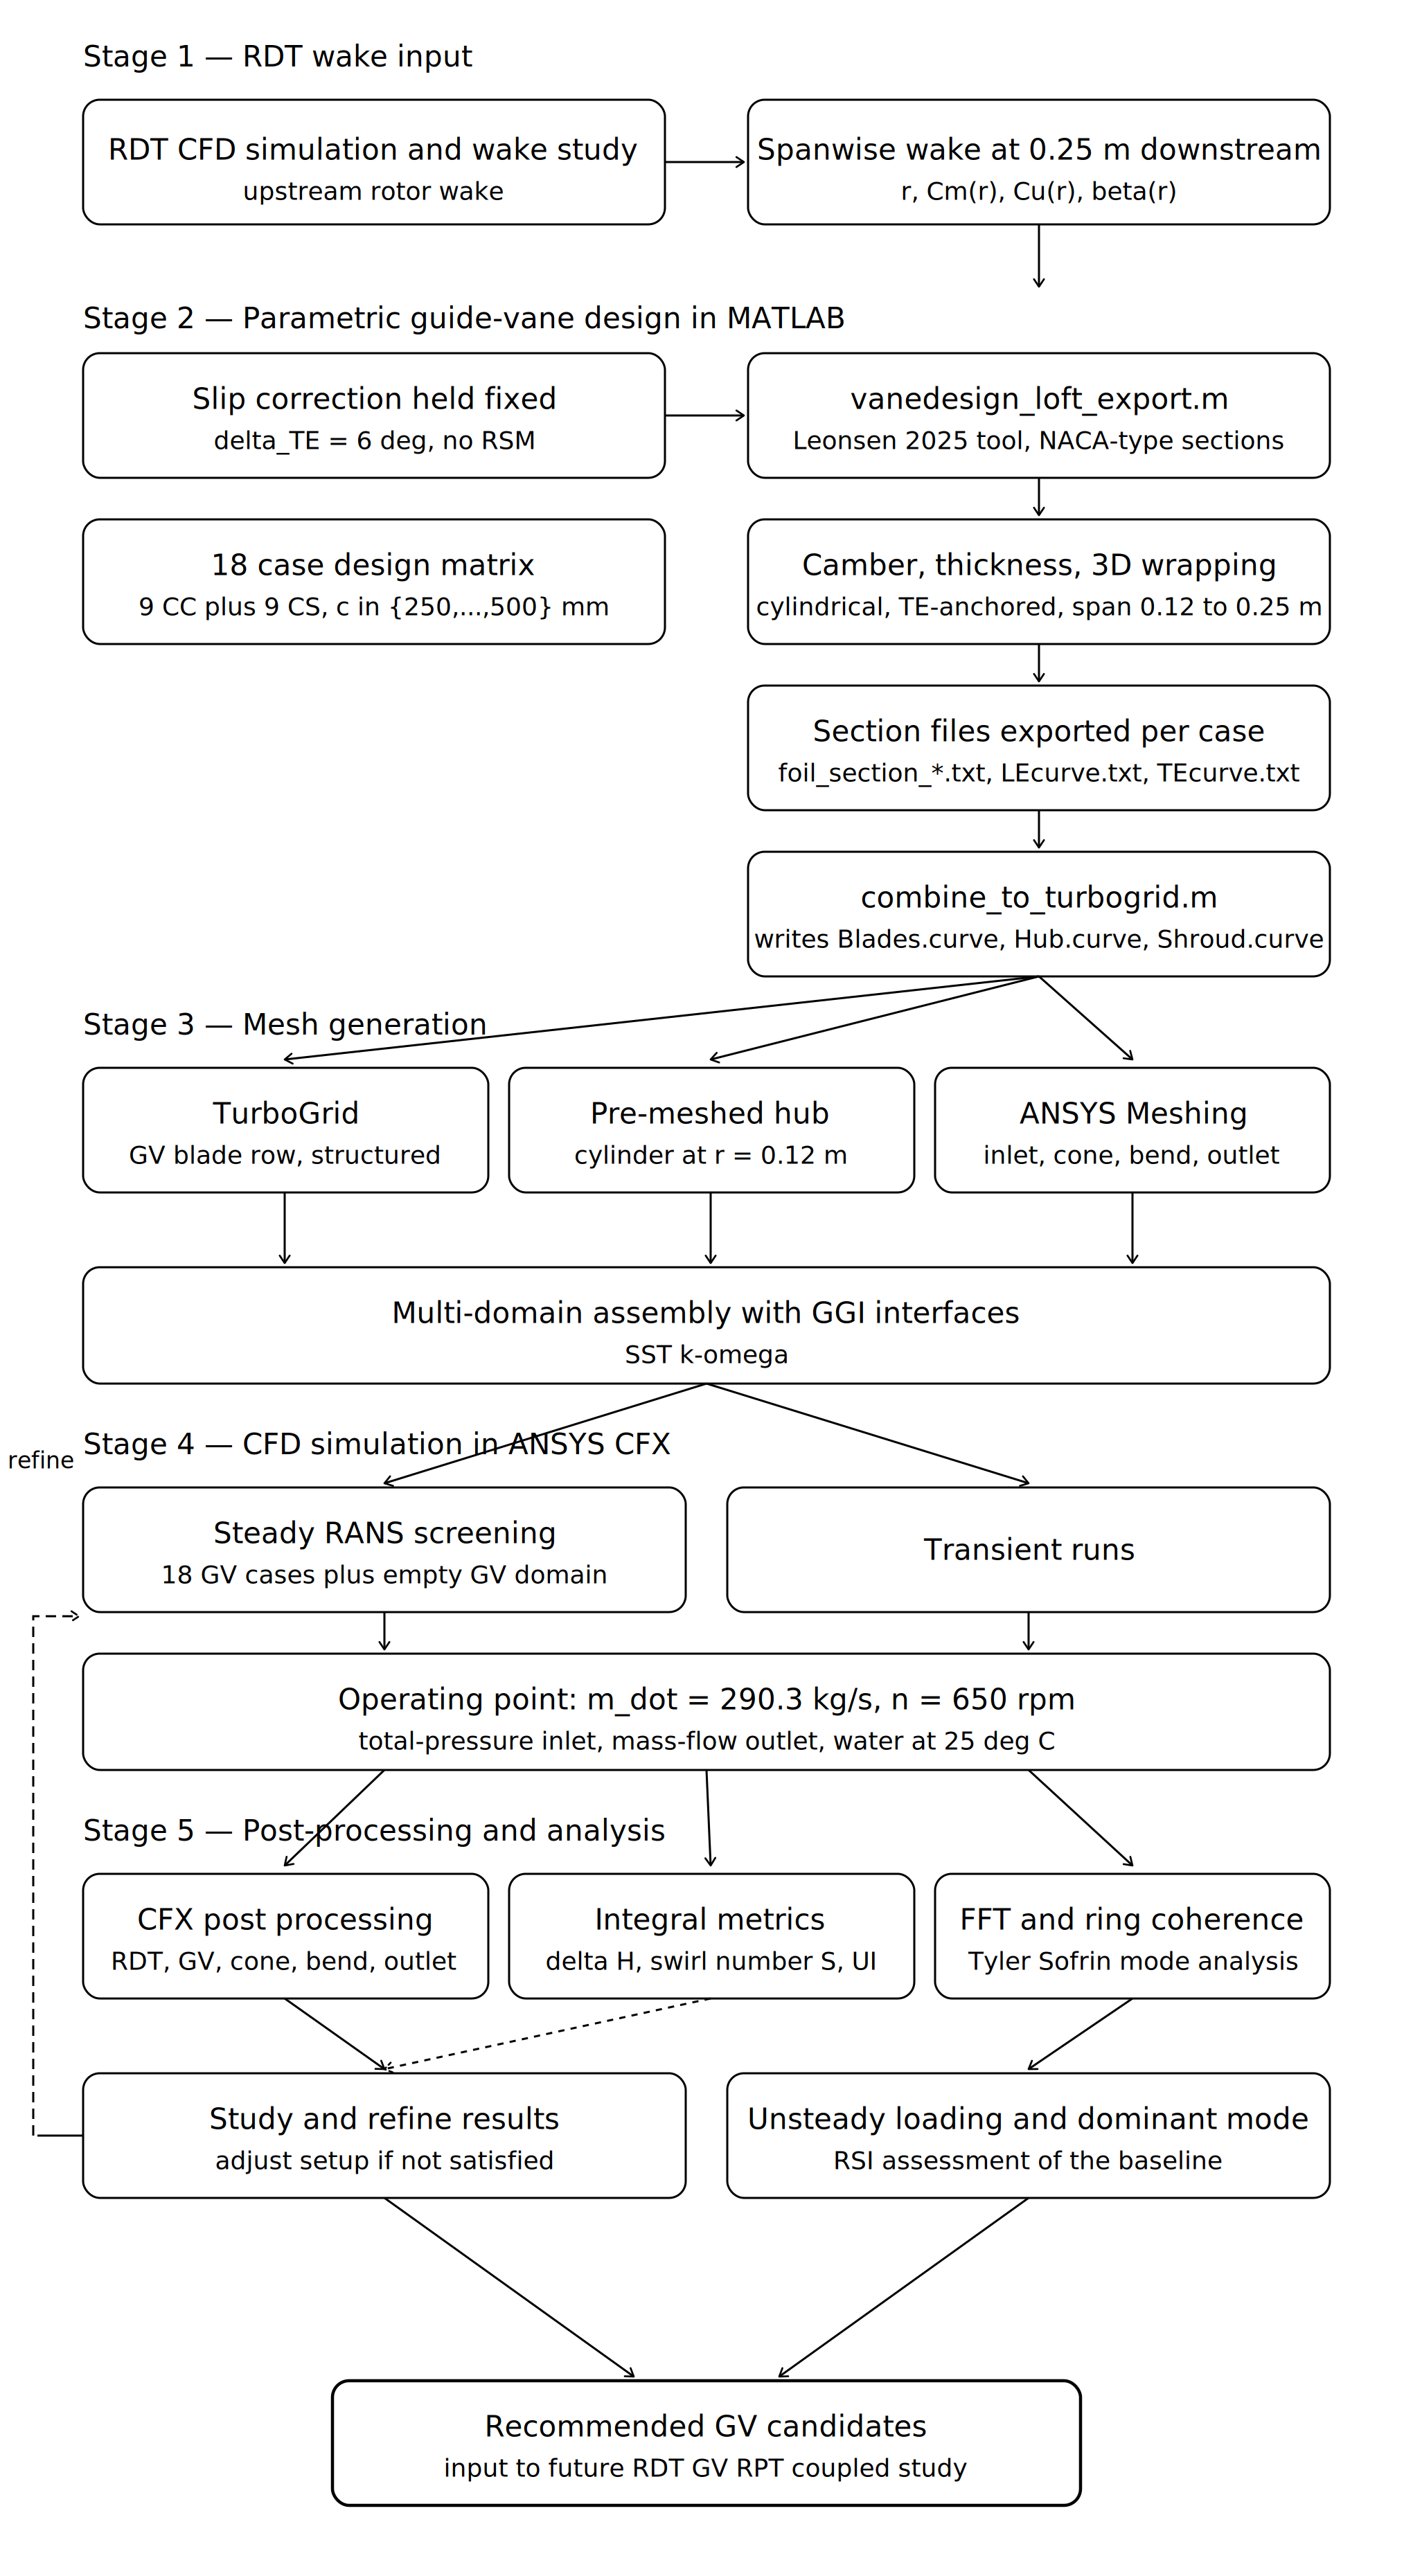
\includegraphics[width=0.7\textwidth]{Figures/FlowChart/Master_full_workflow.png}
  \caption[Methodology overview]{Methodology overview for the 18-case screening campaign and the two transient diagnostic runs. Each configuration follows the same pipeline from MATLAB section generation to CFX simulation and post-processing.}
  \label{fig:methodology_overview}
\end{figure}
 
% ---------------------------------------------------------------------
\section{Parametric guide-vane design tool}
\label{sec:methods_matlab_tool}
 
The guide-vane geometries are generated by the MATLAB tool \texttt{vanedesign\_loft\_export.m} that was developed in the project work~\cite{Leonsen2025}. The tool reads spanwise distributions $\{r,\,C_m(r),\,C_u(r)\}$ from the RDT wake. From these it computes the local inlet flow angle $\alpha_1(r) = \arctan(C_u/C_m)$ and the local diameter-based Reynolds number $\mathrm{Re}_D(r)$. It then constructs the metal angles, the chord distribution, the two-dimensional camber and thickness, and the three-dimensional wrapped vane surface. The geometric construction is described in Section~\ref{sec:theory_geometric_construction}. The output of the tool is a set of section curves and an STL file. In the present thesis, these are converted directly into TurboGrid \texttt{Blades.curve}, \texttt{Hub.curve} and \texttt{Shroud.curve} input files by an auxiliary MATLAB routine. This replaces the Visual Studio and SolidWorks lofting pipeline used in the project work.
 
The tool exposes a structured options list, of which the following are exercised in the screening campaign:
\begin{itemize}
  \item \texttt{Zs}: vane count;
  \item \texttt{use\_sigma}: boolean switching between fixed chord (\texttt{false}) and target solidity (\texttt{true});
  \item \texttt{c\_const\_fallback}: shroud chord when \texttt{use\_sigma = false};
  \item \texttt{sigma\_target}: target solidity at the shroud when \texttt{use\_sigma = true};
  \item \texttt{slip\_choice = 'const'} with \texttt{slip\_const\_deg = 6.0}: fixed slip correction in line with G\"ulich's recommendation~\cite{Gulich2010};
  \item \texttt{tc\_rel = 0.075}, \texttt{tTE\_rel = 0.005}, \texttt{LE\_round = 1.2}: thickness law parameters held constant;
  \item \texttt{use\_cone\_wrap = false}, \texttt{use\_TE\_anchor = true}: cylindrical wrapping with a common trailing-edge azimuth;
  \item \texttt{lean\_amp = 0}, \texttt{sweep\_amp = 0}: lean and sweep held at zero in the screening campaign.
\end{itemize}
 
\paragraph{Choice of slip-correction strategy.}
The project work~\cite{Leonsen2025} developed a CFD-based slip database and a smooth response-surface model that predicts deviation as a function of inlet flow angle and Reynolds number. At the high turning angles required to recover the RDT swirl, this response surface predicts deviation values on the order of $10^\circ$-$20^\circ$. Adopting these large built-in trailing-edge angles aggressively over-cambers the section near the trailing edge, sharpens the suction-side adverse pressure gradient, and tends to promote separation. The classical recommendation by G\"ulich~\cite{Gulich2010} is more conservative: a small built-in angle of approximately $4^\circ$-$6^\circ$ is sufficient to compensate for cascade deviation in well-designed pump and stator vanes. The present screening campaign adopts the upper end of this range, $\delta_{\mathrm{TE}} = 6^\circ$, applied as a constant correction to the trailing-edge metal angle for every section across all 18 configurations. This choice reduces one degree of freedom in the screening campaign and isolates the chord-strategy and vane-count effects that the master thesis is designed to study. The trade-off between aggressive slip correction (response surface) and conservative slip correction (G\"ulich) is acknowledged as a question that could be revisited in a focused follow-up study using a small subset of the screening configurations.
 
\paragraph{Spanwise inlet data.}
The spanwise distributions $\{r,\,C_m(r),\,C_u(r)\}$ used as the design input are taken from the RDT simulation of Djupesland and Trivedi~\cite{DjupeslandTrivedi2025}, evaluated at a plane $0.25$~m downstream of the rotor. The valid design span is restricted to radii with positive meridional velocity. As discussed in Section~\ref{sec:theory_backflow_span}, this corresponds approximately to $r \in [0.12, 0.25]$~m, which is the radial extent of all guide vanes used in the screening campaign.
 
% ---------------------------------------------------------------------
\section{Design matrix: 18 configurations}
\label{sec:methods_design_matrix}
 
The design space is sampled on a structured matrix of 18 configurations that combines two chord-control strategies, six shroud-chord levels and three vane counts. The matrix is symmetric: every constant-chord (CC) configuration has a constant-solidity (CS) twin at the same shroud chord and vane count, which isolates the effect of the chord-control strategy from the effect of loading. A nineteenth simulation, denoted \texttt{NoGV}, replaces the guide-vane region with an empty straight pipe of equal length and serves as the swirl-reduction reference against which all 18 configurations are compared (Section~\ref{sec:methods_rdt_baseline}).
 
\paragraph{Choice of two chord-control strategies.}
The two chord-control strategies are the simplest non-trivial laws for how the local chord scales with radius, and both are natively supported by the parametric tool of Leonsen~\cite{Leonsen2025}. Constant chord (CC) keeps $c(r)$ fixed across the span, so the local solidity $\sigma(r) = Z_s\, c(r) / (2\pi r)$ scales as $1/r$ and increases sharply near the hub. Constant solidity at the shroud (CS) instead lets $c(r)$ scale linearly with $r$, so $\sigma(r)$ stays at the shroud value across the span. Together with the three vane counts $Z_s \in \{6, 8, 9\}$, these two laws span the loading regimes reachable with a single hubless cascade family. More elaborate strategies (taper, sweep, lean) are excluded from the screening to keep the parameter space interpretable and the case count manageable.
 
The case-naming convention used throughout this thesis is
 
\medskip
\centerline{\texttt{<strategy>\_<chord shroud in mm>\_<Z\_s>}}
\medskip
 
\noindent
where \texttt{strategy} is either \texttt{CC} (constant chord) or \texttt{CS} (constant solidity at the shroud), the second field is the chord at the shroud in millimetres, and the third field is the vane count $Z_s$. For example, \texttt{CC\_400\_8} denotes a constant-chord configuration with $c = 400$~mm at all radii and $Z_s = 8$ vanes. \texttt{CS\_400\_8} denotes a constant-solidity configuration with $c(r=0.25) = 400$~mm at the shroud and chord scaling linearly with $r$ inwards, to preserve solidity. The full list of configurations is given in Table~\ref{tab:design_matrix}.
 
\begin{table}[h!]
  \centering
  \caption[Design matrix used in the screening campaign]%
  {Design matrix used in the screening campaign. CC denotes constant chord; CS denotes constant solidity referenced at the shroud. All 18 configurations are simulated at $\dot m = 290.3$~kg/s and $n = 650$~rpm with the same RDT inlet wake and the same downstream draft-tube geometry. The \texttt{NoGV} reference simulation uses the identical domain with the guide-vane region replaced by an empty straight pipe.}
  \label{tab:design_matrix}
  \small
  \begin{tabular}{l|c|c|c}
    \toprule
    \textbf{Case ID} & \textbf{Strategy} & $c_{\mathrm{shroud}}$ (mm) & $Z_s$ \\
    \midrule
    CC\_250\_9  & Constant chord    & 250 & 9 \\
    CC\_300\_9  & Constant chord    & 300 & 9 \\
    CC\_350\_8  & Constant chord    & 350 & 8 \\
    CC\_400\_6  & Constant chord    & 400 & 6 \\
    CC\_400\_8  & Constant chord    & 400 & 8 \\
    CC\_450\_6  & Constant chord    & 450 & 6 \\
    CC\_450\_8  & Constant chord    & 450 & 8 \\
    CC\_500\_6  & Constant chord    & 500 & 6 \\
    CC\_500\_8  & Constant chord    & 500 & 8 \\
    \midrule
    CS\_250\_9  & Constant solidity & 250 & 9 \\
    CS\_300\_9  & Constant solidity & 300 & 9 \\
    CS\_350\_8  & Constant solidity & 350 & 8 \\
    CS\_400\_6  & Constant solidity & 400 & 6 \\
    CS\_400\_8  & Constant solidity & 400 & 8 \\
    CS\_450\_6  & Constant solidity & 450 & 6 \\
    CS\_450\_8  & Constant solidity & 450 & 8 \\
    CS\_500\_6  & Constant solidity & 500 & 6 \\
    CS\_500\_8  & Constant solidity & 500 & 8 \\
    \midrule
    \texttt{NoGV} & No guide vanes (reference) & - & - \\
    \bottomrule
  \end{tabular}
\end{table}
 
\paragraph{Coverage and rationale.}
The matrix covers the six shroud-chord levels $\{250, 300, 350, 400, 450, 500\}$~mm and the vane counts $\{6, 8, 9\}$. Vane count and chord are paired as follows. $Z_s = 9$ is paired with the smaller chords $\{250, 300\}$~mm. $Z_s = 8$ spans $\{350, 400, 450, 500\}$~mm. $Z_s = 6$ covers $\{400, 450, 500\}$~mm. Dense short-chord arrangements probe the high-blockage regime: per-vane loading is moderate but total wetted area is large. Sparse long-chord arrangements probe the opposite: per-vane loading is high, blockage is moderate. The symmetric pairing between the CC and CS branches isolates the effect of the chord-control strategy at fixed $(c_{\mathrm{shroud}}, Z_s)$. Configurations that would lie close to the boundaries of the trade-off, e.g.\ very low solidity at high $Z_s$ that would behave essentially as a high-loss screen, are deliberately excluded.
 
\paragraph{Constants across the matrix.}
All 18 configurations and the \texttt{NoGV} reference share the same constants, so that the only differences between the GV configurations are the design variables in Table~\ref{tab:design_matrix}. The constants are: thickness ratio $(t/c)_{\mathrm{rel}} = 0.075$; trailing-edge thickness $t_{\mathrm{TE}}/c = 0.005$; leading-edge roundness factor $\texttt{LE\_round} = 1.2$; slip correction $\delta_{\mathrm{TE}} = 6^\circ$; cylindrical wrapping; trailing-edge anchoring at a common azimuth; and design span $r \in [0.12, 0.25]$~m. Operating conditions are held fixed at $\dot m = 290.3$~kg/s, $n = 650$~rpm, water at $25^\circ$C.

\paragraph{Two additional transient runs.}
In addition to the 18 steady configurations of Table~\ref{tab:design_matrix} and the \texttt{NoGV} reference, two extra simulations are run in transient mode for the rotor-stator interaction analysis (Sections~\ref{sec:rsi-thesis} and~\ref{sec:monitor-setup}-\ref{sec:spec-coherence}). The first is \texttt{CC\_450\_7}, which corresponds to the project-work baseline geometry with $Z_r=Z_s=7$ and is the reference for the synchronous Tyler-Sofrin breathing mode ($m_{\min}=0$). The second is \texttt{CC\_400\_6}, used as the $m_{\min}\geq 1$ counterpart from the screening matrix; the choice of \texttt{CC\_400\_6} rather than \texttt{CC\_450\_6} is motivated in the closing paragraph of Section~\ref{sec:rsi-thesis}. Both transient runs use the same multi-domain CFX setup, mesh strategy and operating point as the steady screening campaign, with the rotor-stator interfaces switched from frozen rotor to transient rotor-stator (Section~\ref{sec:methods_bc}, Section~\ref{sec:monitor-setup}).

% ---------------------------------------------------------------------
\section{Design-space visualisation}
\label{sec:methods_design_space_viz}

The design matrix in Table~\ref{tab:design_matrix} is summarised graphically in Figures~\ref{fig:design_space_overview}-\ref{fig:reference_card}. The four plots together show three things. They visualise where the 18 active configurations sit in the loading-chord plane. They show how the constant-chord and constant-solidity strategies differ in radial loading. They compare the cases against the recommended cascade-loading bound $\sigma \lesssim 1.6$, adopted as a soft design guideline in axial-pump and stator design~\cite{Gulich2010}.

Figure~\ref{fig:design_space_overview} plots all configurations in the $(\sigma_{\mathrm{shroud}},\,c_{\mathrm{shroud}})$ plane. The 18 active configurations of the screening campaign are marked in colour. Greyed-out points show the corresponding $Z_s = 7$ designs, included for context only. These coincide with the original project-work baseline ($Z_r = Z_s = 7$) and are excluded from the screening on Tyler-Sofrin grounds (Section~\ref{sec:rsi-thesis}). The dashed vertical line at $\sigma_{\mathrm{shroud}} = 1.6$ separates the recommended-loading region from the over-loaded region. Only the smallest active configurations (\texttt{CC\_250\_9}, \texttt{CS\_250\_9}, \texttt{CC\_400\_6}, \texttt{CS\_400\_6}) sit close to or inside the recommended region at the shroud; the remainder of the matrix is loaded above this guideline at the shroud.

\begin{figure}[h!]
  \centering
  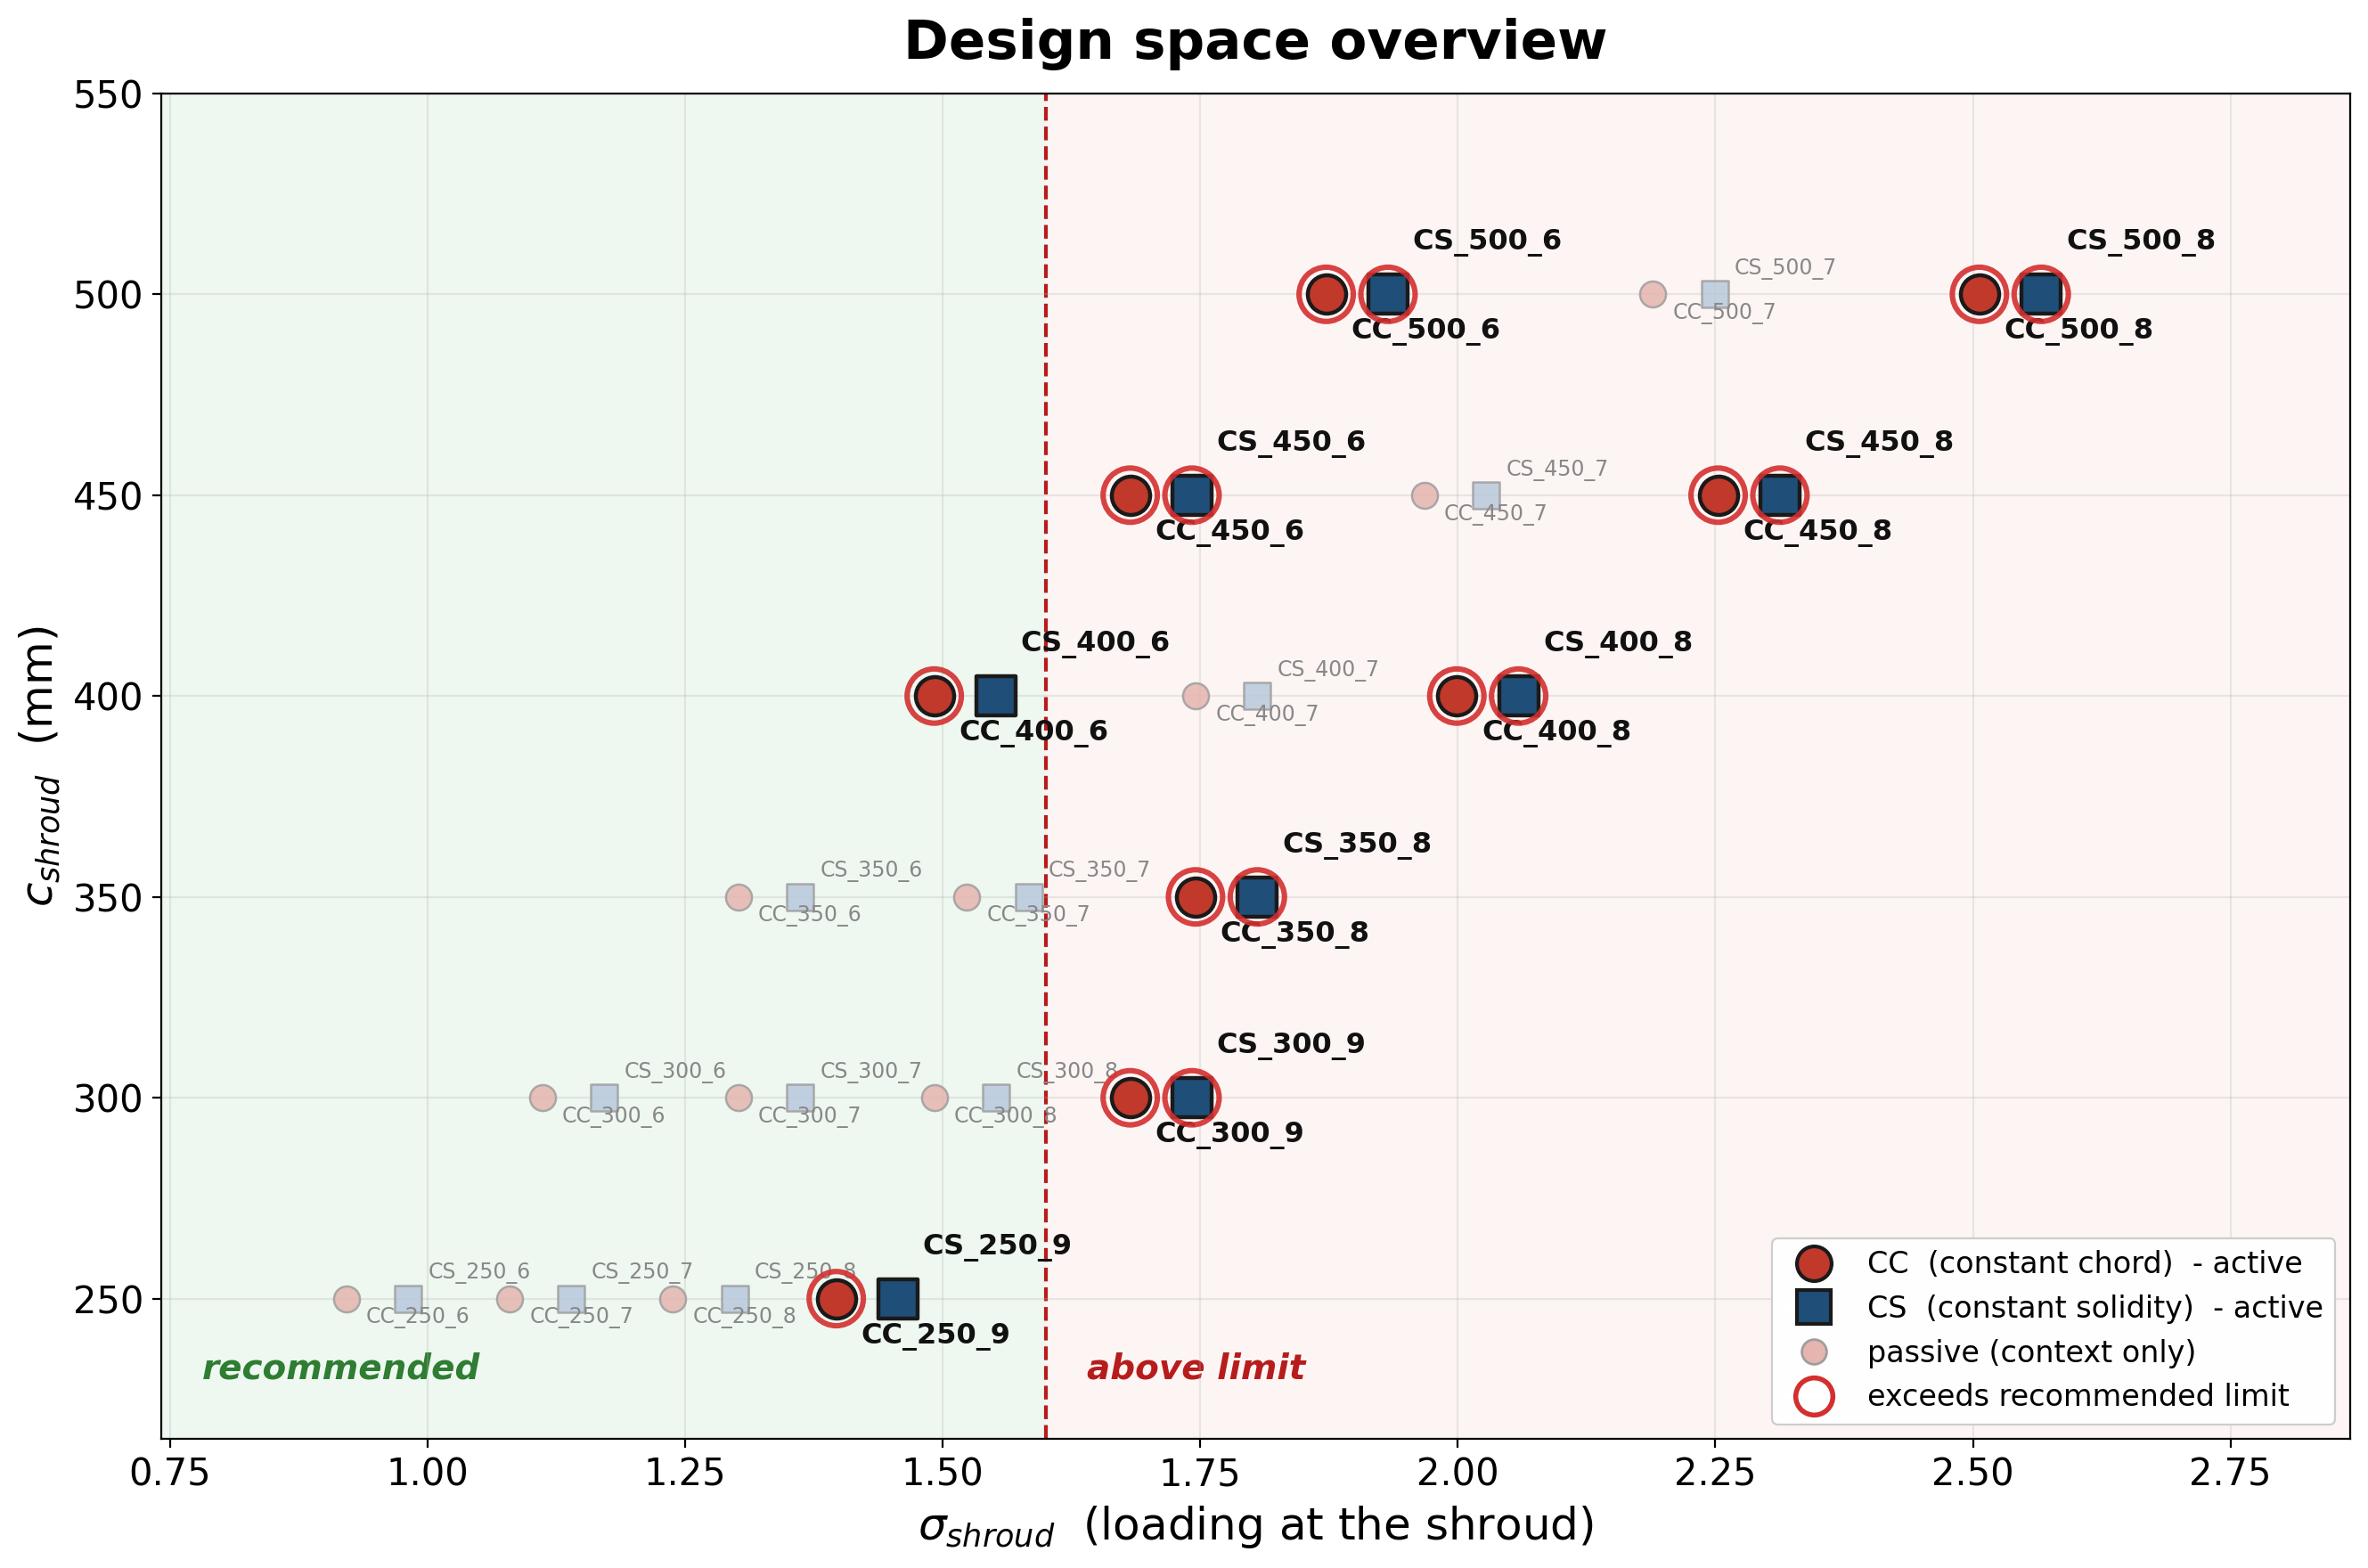
\includegraphics[width=0.95\textwidth]{Figures/GV_Design/Design_plots/fig1_master_design_space.png}
  \caption[Design-space overview]{Design-space overview of the 18 active configurations. Constant-chord (CC) cases are red circles, constant-solidity (CS) cases are blue squares. Greyed points are the inactive $Z_s = 7$ context cases. The dashed vertical line at $\sigma_{\mathrm{shroud}} = 1.6$ separates the recommended region (green) from the above-limit region (red) following the soft cascade-loading guideline of G\"ulich~\cite{Gulich2010}. Most of the matrix is intentionally loaded beyond the conventional limit, because the high turning required to recover the RDT swirl forces the design into this regime.}
  \label{fig:design_space_overview}
\end{figure}

Figure~\ref{fig:hub_vs_shroud} compares the local solidity at the hub of the design span ($r = 0.12$~m) with the local solidity at the shroud ($r = 0.25$~m). For the constant-solidity (CS) family the chord is by construction proportional to $r$, so $\sigma_{\mathrm{hub}} = \sigma_{\mathrm{shroud}}$ and all CS points lie on the diagonal. For the constant-chord (CC) family the same chord is used at every radius, so $\sigma_{\mathrm{hub}} = \sigma_{\mathrm{shroud}}\,(R_{\mathrm{shroud}}/R_{\mathrm{hub}}) \approx 2.08\,\sigma_{\mathrm{shroud}}$, and all CC points lie above the diagonal. The figure quantifies the central design distinction between the two families: a CC vane is more heavily loaded near the hub than near the shroud, while a CS vane has uniform loading along the span. The horizontal dashed line at $\sigma_{\mathrm{hub}} = 1.6$ shows that all CC configurations exceed the recommended hub loading, by a factor of two or more for the largest cases. CS configurations remain within or close to the limit at the hub if and only if they are within the limit at the shroud.

\begin{figure}[h!]
  \centering
  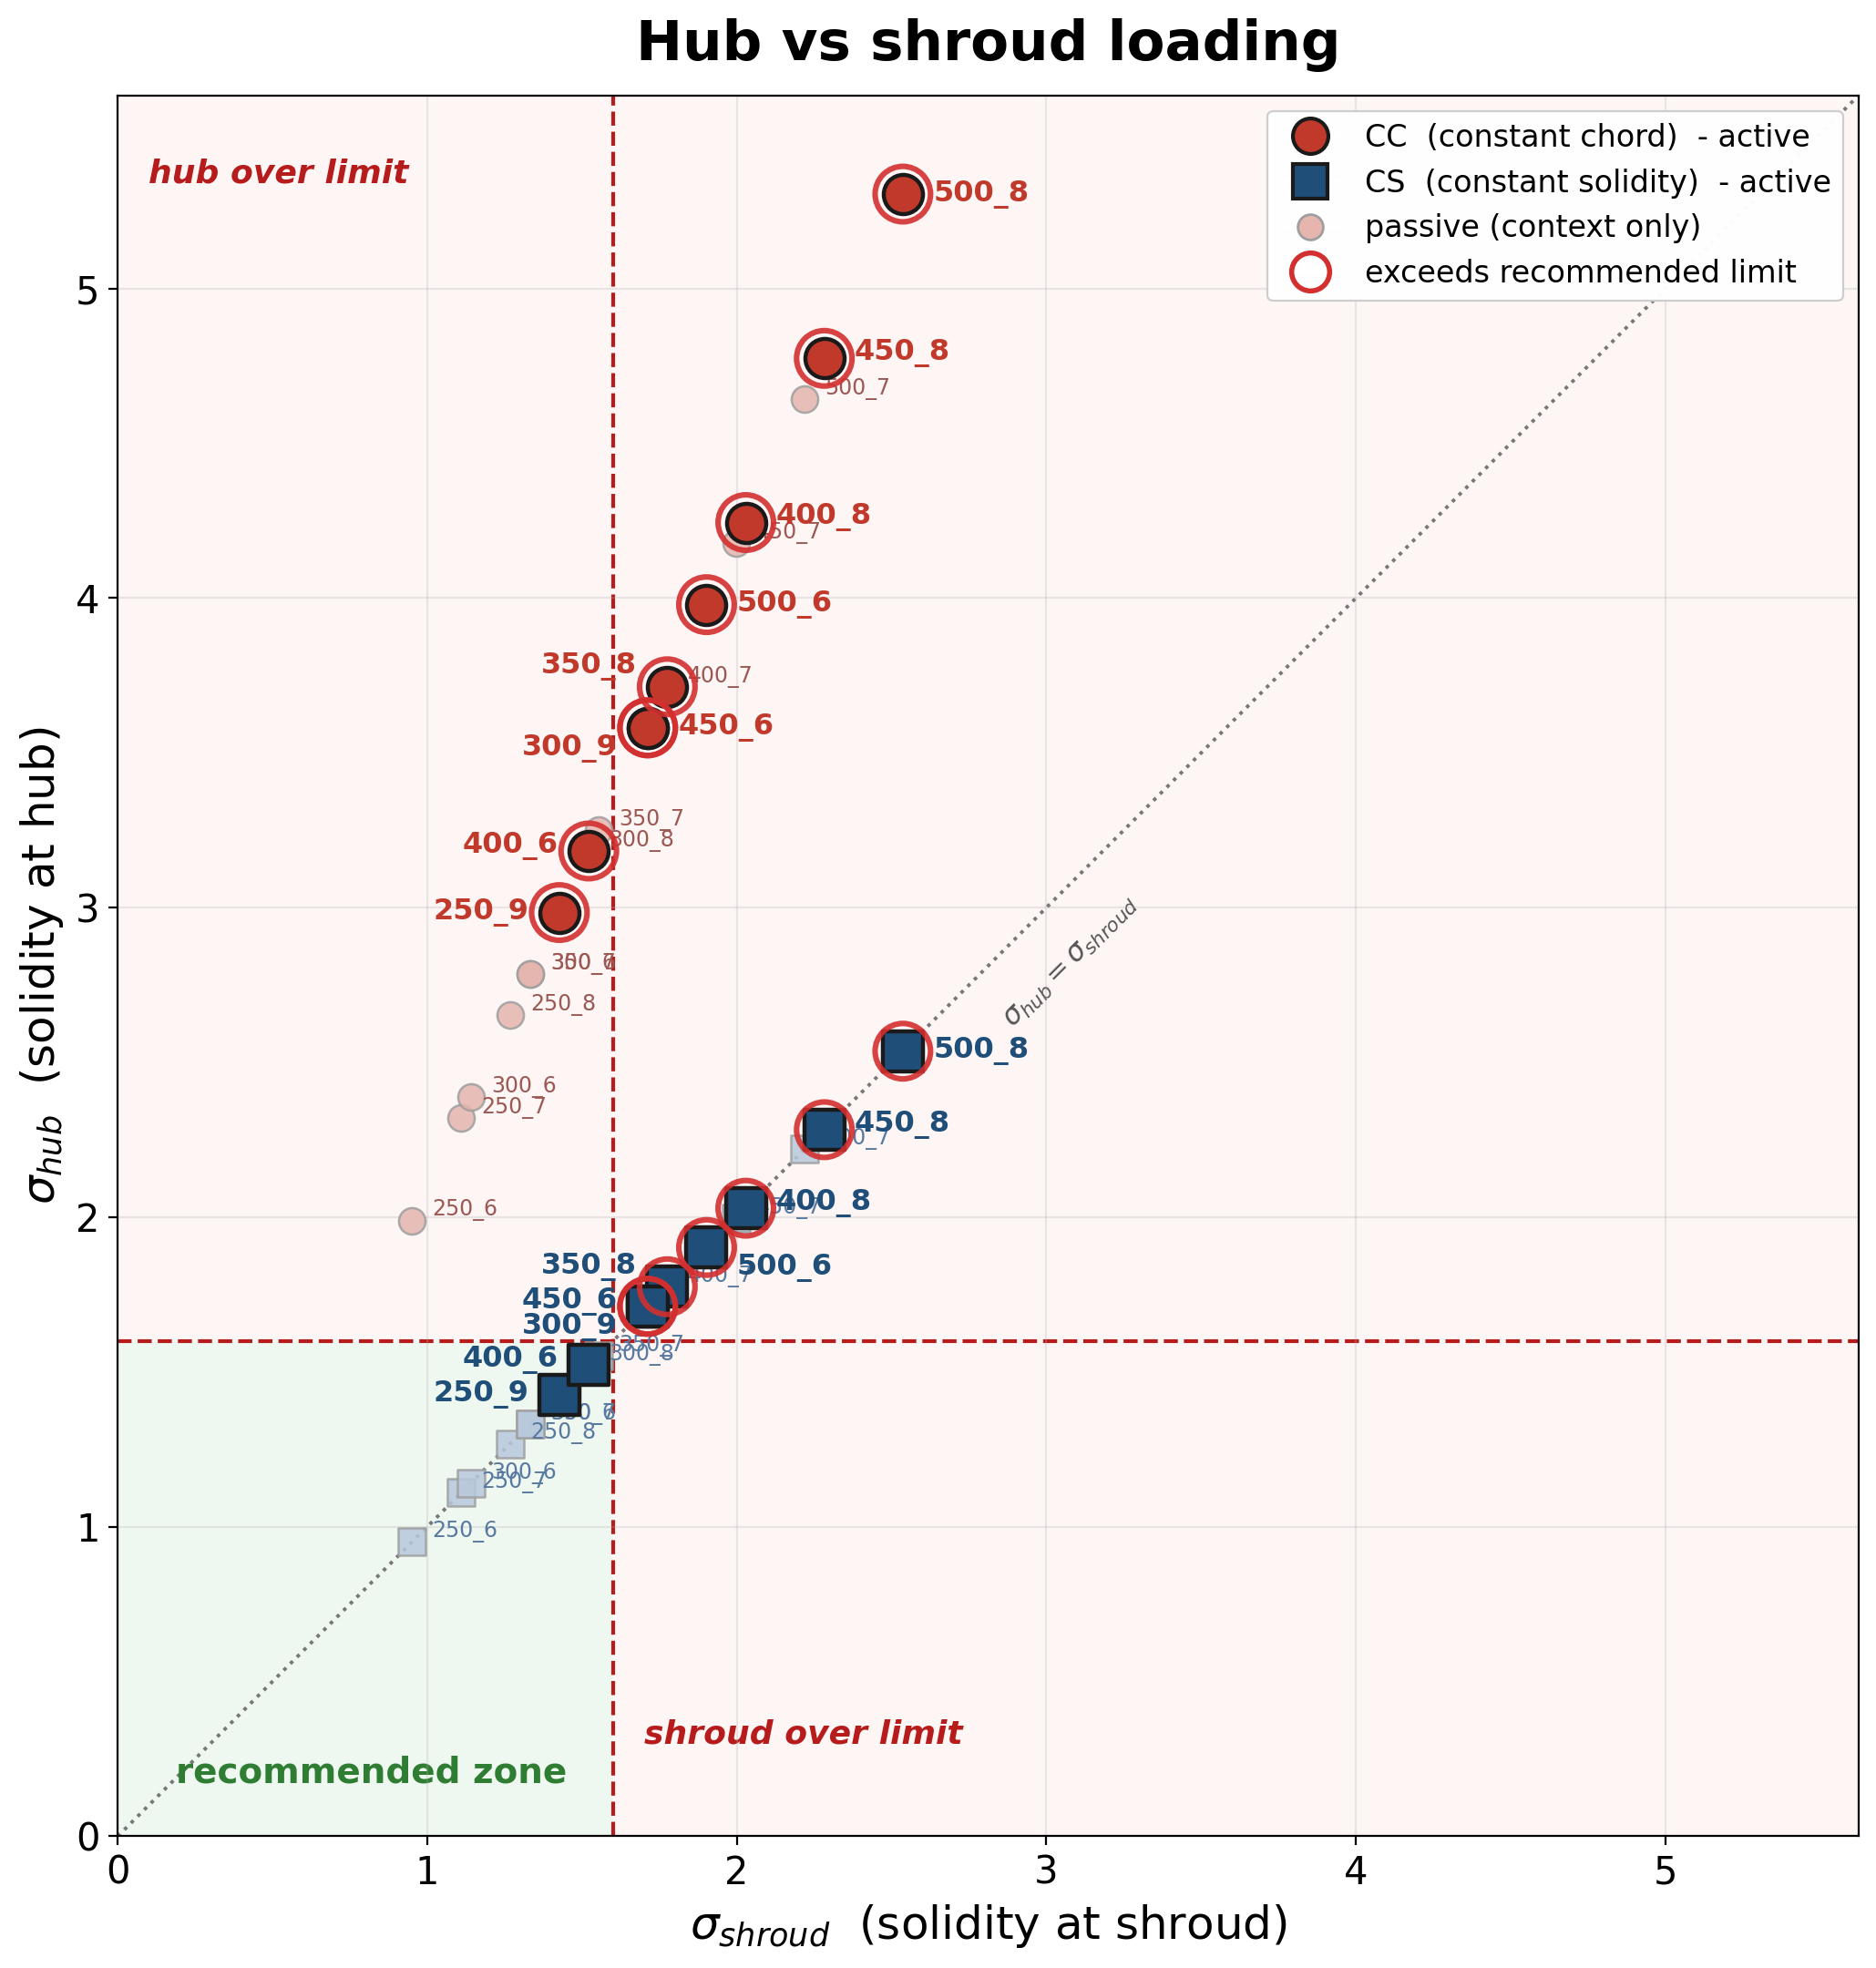
\includegraphics[width=0.95\textwidth]{Figures/GV_Design/Design_plots/fig2_hub_vs_shroud.png}
  \caption[Hub vs shroud loading]{Hub solidity $\sigma_{\mathrm{hub}}$ versus shroud solidity $\sigma_{\mathrm{shroud}}$ for the 18 active configurations. CS cases lie on the diagonal $\sigma_{\mathrm{hub}} = \sigma_{\mathrm{shroud}}$. CC cases lie on the steeper line $\sigma_{\mathrm{hub}} \approx 2.08\,\sigma_{\mathrm{shroud}}$ because the same chord is used at every radius. The recommended-loading limit $\sigma \lesssim 1.6$ is exceeded at the hub by every CC configuration in the matrix.}
  \label{fig:hub_vs_shroud}
\end{figure}

Figure~\ref{fig:radial_solidity} traces the local solidity $\sigma(r) = c(r)Z_s/(2\pi r)$ across the design span $r \in [0.12, 0.25]$~m for all chord and vane-count combinations. The CC profiles fall hyperbolically with $r$ (solid lines), while the CS profiles are flat in $r$ (dashed lines) by construction. The figure shows where the high-$\sigma$ regions sit on each design and is the radial-resolved counterpart of the two scalar plots above.

\begin{figure}[h!]
  \centering
  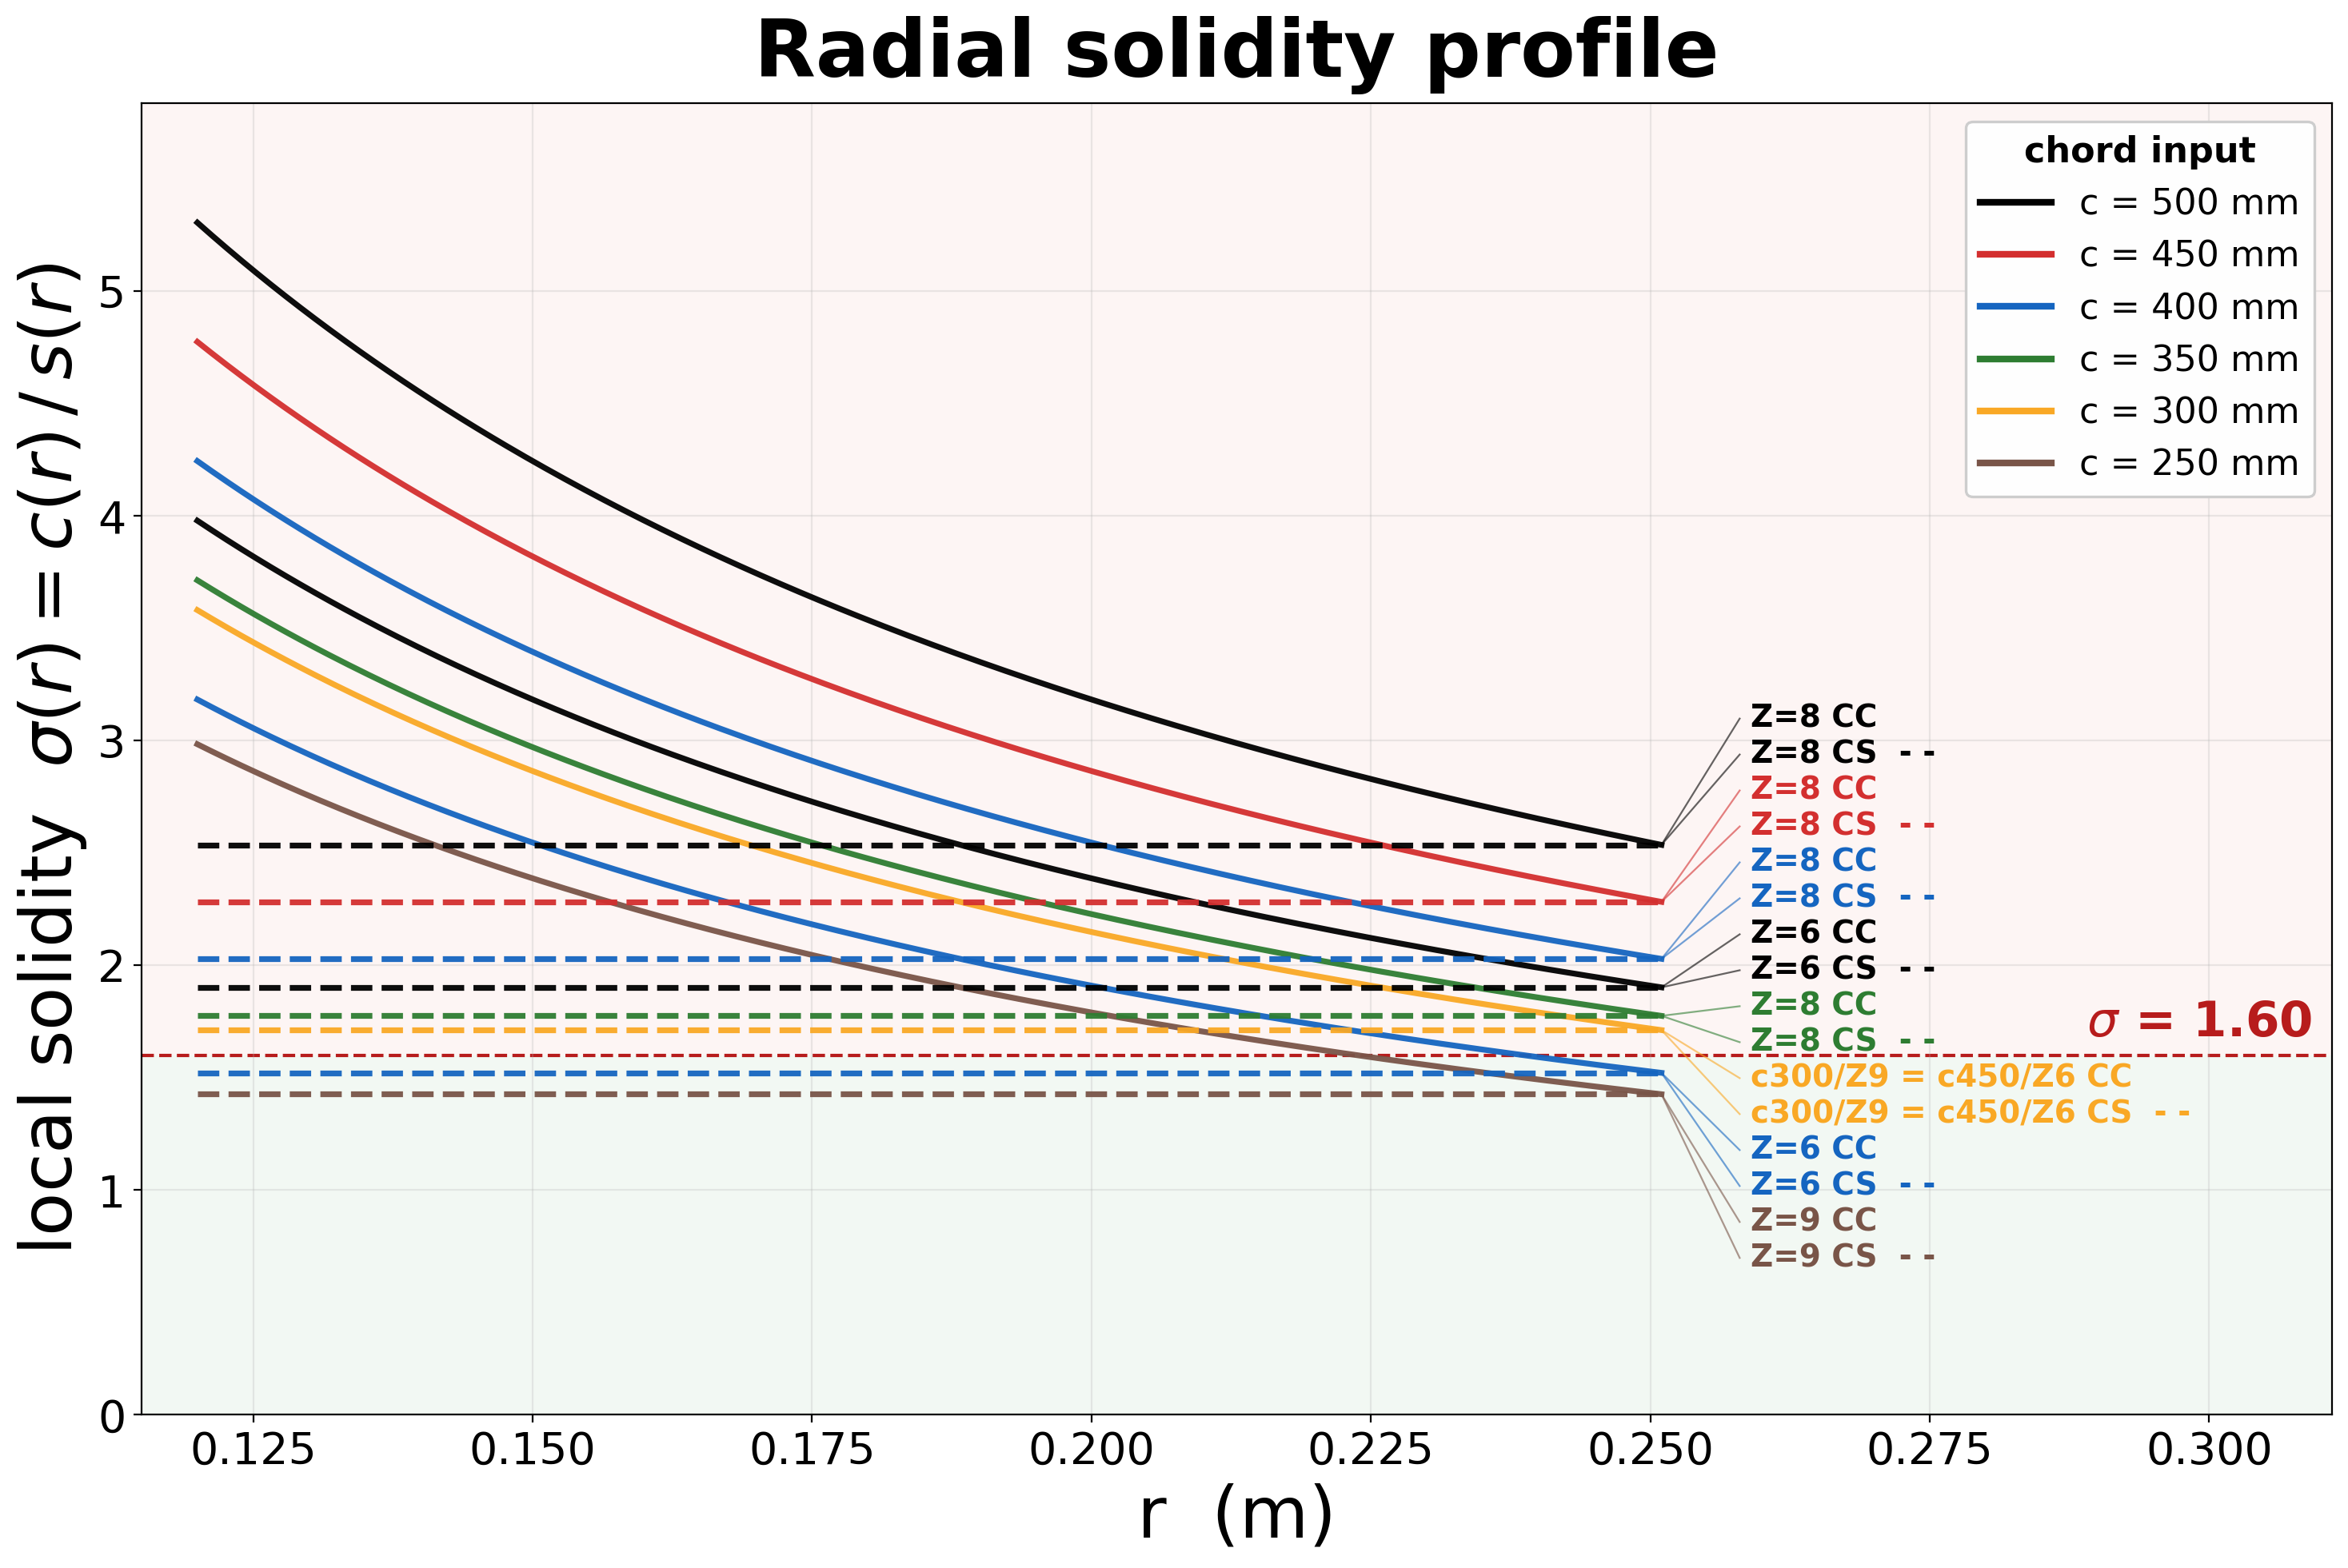
\includegraphics[width=0.99\textwidth]{Figures/GV_Design/Design_plots/fig3_radial_solidity.png}
  \caption[Radial solidity profile]{Radial profile of the local solidity $\sigma(r) = c(r)Z_s/(2\pi r)$ across the design span $r \in [0.12, 0.25]$~m for all chord and vane-count combinations. Solid lines: constant-chord (CC) family, with $\sigma$ falling hyperbolically with $r$. Dashed lines: constant-solidity (CS) family, with $\sigma$ uniform in $r$ by construction. The dashed red horizontal line marks the soft loading guideline $\sigma = 1.6$.}
  \label{fig:radial_solidity}
\end{figure}

Figure~\ref{fig:reference_card} sorts the 18 active configurations by hub solidity $\sigma_{\mathrm{hub}}$ in ascending order and lists the chord at the hub $c_{\mathrm{hub}}$, the chord at the shroud $c_{\mathrm{shroud}}$, and the local solidities at hub, mid-span and shroud. Cells are colour-coded against the soft loading guideline (yellow when $\sigma \leq 1.6$, pink when above). The card is used as a quick reference in the discussion of the screening results in Chapter~\ref{chap:results_discussion}. \texttt{CS\_250\_9} is the only configuration that sits inside the recommended region at every span, with $\sigma = 1.43$ uniform. \texttt{CS\_400\_6} is just inside the limit at $\sigma = 1.52$ uniform. The remaining 16 configurations exceed the recommended loading at the hub. The worst case is \texttt{CC\_500\_8}, which reaches $\sigma_{\mathrm{hub}} = 5.31$.

\begin{figure}[h!]
  \centering
  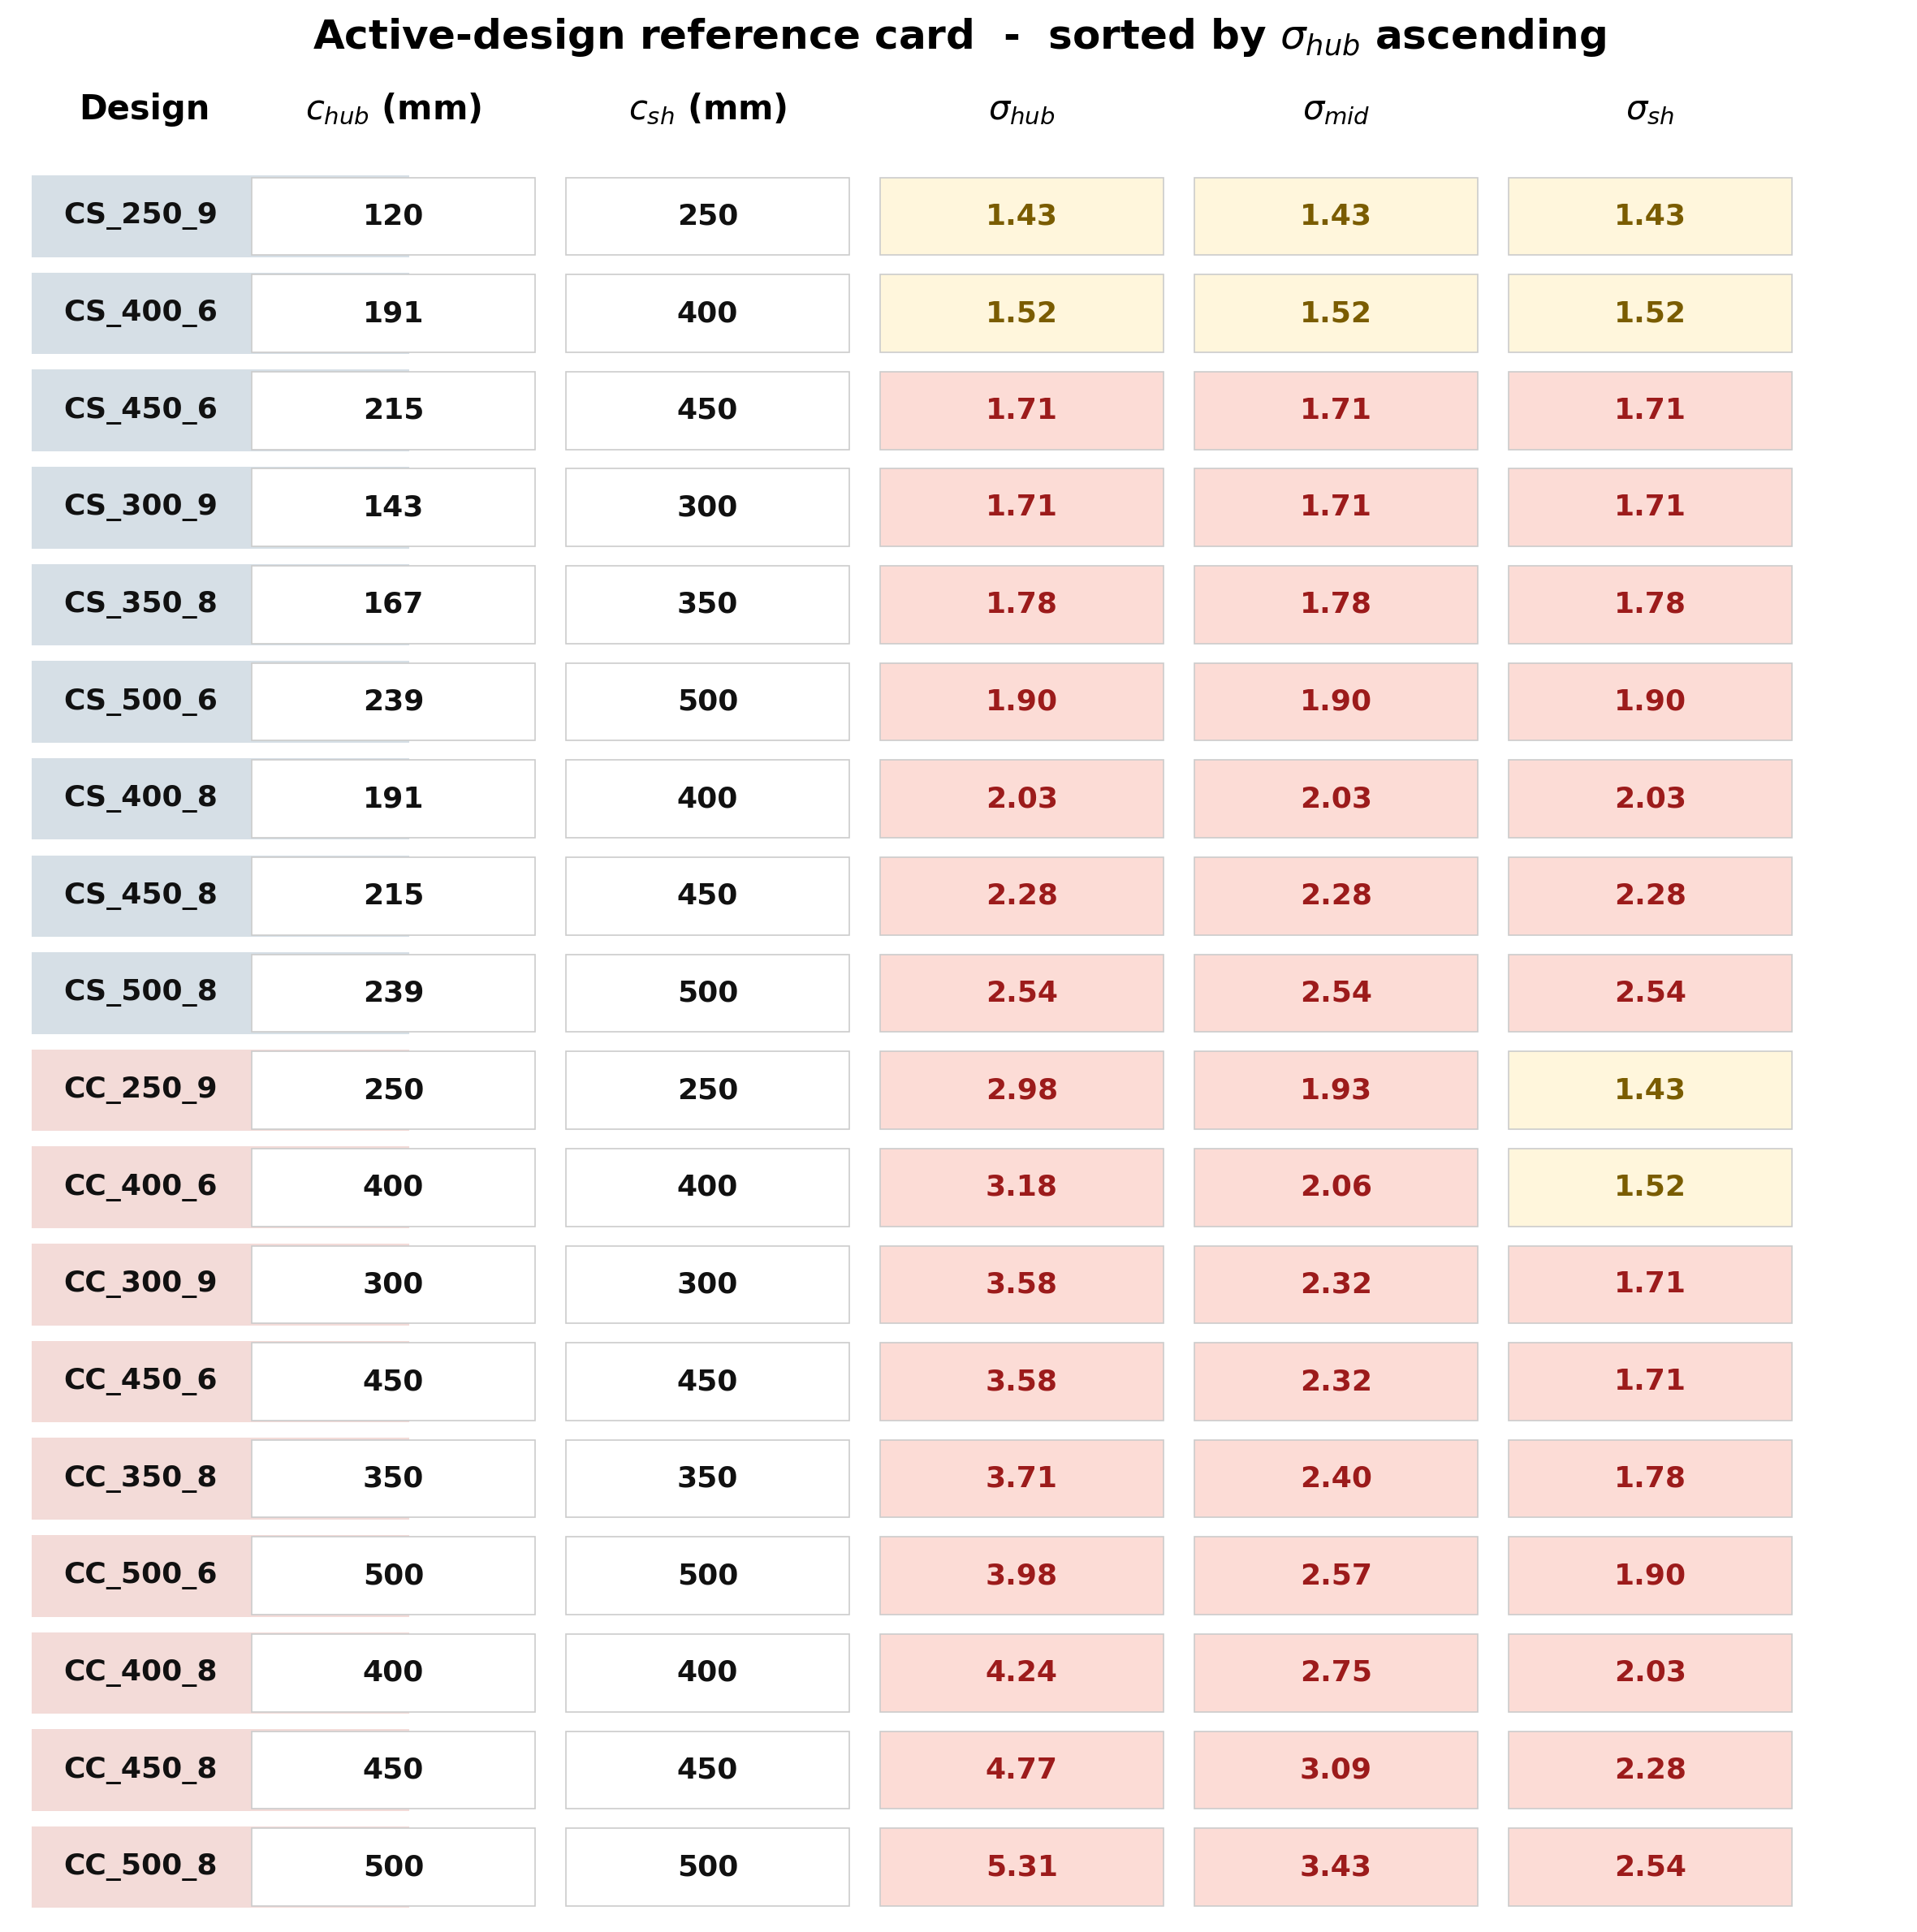
\includegraphics[width=0.95\textwidth]{Figures/GV_Design/Design_plots/fig4_reference_card.png}
  \caption[Active-design reference card]{Active-design reference card sorted by hub solidity $\sigma_{\mathrm{hub}}$ in ascending order. Columns: case identifier, chord at the hub $c_{\mathrm{hub}}$, chord at the shroud $c_{\mathrm{shroud}}$, and the local solidities at hub, mid-span and shroud. Yellow cells are within the recommended loading guideline $\sigma \leq 1.6$; pink cells are above.}
  \label{fig:reference_card}
\end{figure}

\paragraph{Implication of the high-$\sigma$ region.}
The diffusion-factor and de Haller bounds are, in this geometry, indicative rather than binding. They are exceeded over part of the span by every active configuration because the very high RDT outflow angles ($\alpha > 80^\circ$ in the outer span; Section~\ref{sec:methods_rdt_velocity_triangles}) require a large flow turning that cannot be delivered with $\sigma \lesssim 1.6$ along the full span. The screening campaign accepts this and uses the bounds as comparative loading indicators, in line with established practice for highly loaded axial machines~\cite{Schnoes2018, Leonsen2025}. The four figures above support the interpretation of the CFD results in Chapter~\ref{chap:results_discussion} by making explicit which configurations are loaded the most aggressively and where on the span this loading is concentrated.

% ---------------------------------------------------------------------
\section{Computational domain and boundary conditions}
\label{sec:methods_domain}
 
The computational domain reproduces the planned Store2Hydro layout from the RDT inlet down to the location where the RPT inlet would be. Six contiguous regions are connected through stationary-stationary or rotating-stationary interfaces. The overall layout is shown in Figure~\ref{fig:domain_layout}, and the regions are listed in Table~\ref{tab:domains}.

\begin{figure}[h!]
  \centering
  \fbox{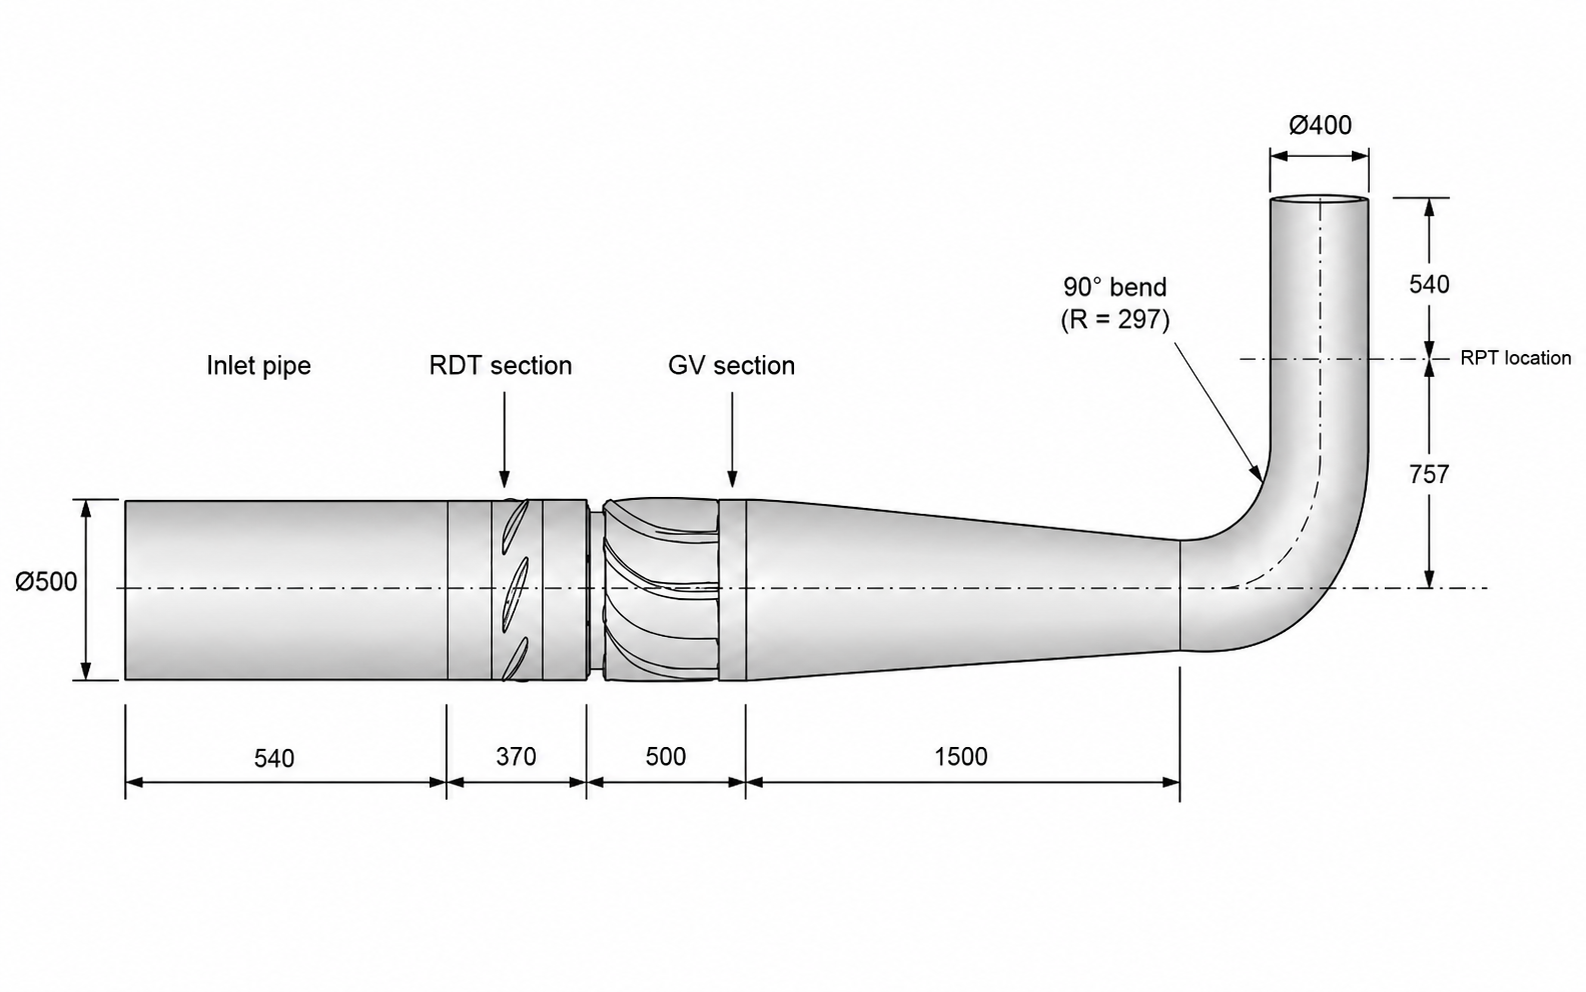
\includegraphics[width=0.95\textwidth]{Figures/2D_drawing/2d_drawing_full_domain.png}}
  \caption[Computational domain layout]{Overview of the computational domain with main dimensions in mm. The inlet pipe ($D = 500$~mm) feeds into the RDT section, followed by the GV section, a $1500$~mm straight section, the $90^\circ$ bend ($R = 297$~mm), and the final straight pipe ($D = 400$~mm) ending at the RPT location. The GV section is the only region that changes between cases in the screening matrix.}
  \label{fig:domain_layout}
\end{figure}
 
\begin{table}[h!]
  \centering
  \caption[Domain regions]{Regions of the multi-domain CFX setup, in flow direction.}
  \label{tab:domains}
  \small
  \begin{tabular}{c|l|l}
    \toprule
    \textbf{Region} & \textbf{Description} & \textbf{Mesh tool} \\
    \midrule
    1 & Inlet pipe, $D = 0.5$~m, length $0.5$~m   & ANSYS Meshing (unstructured) \\
    2 & RDT rotor, $Z_r = 7$ blades              & ANSYS TurboGrid (structured) \\
    3 & Guide-vane row (case-dependent)          & ANSYS TurboGrid (structured) \\
    4 & Inner-pipe section, $r < 0.12$~m         & ANSYS Meshing (structured hub) \\
    5 & Conical contraction, $D = 0.5 \to 0.4$~m & ANSYS Meshing (unstructured) \\
    6 & Draft tube: $90^\circ$ bend + final straight pipe ($\sim 1.0$~m) & ANSYS Meshing (unstructured) \\
    \bottomrule
  \end{tabular}
\end{table}
 
\paragraph{Reasons for the extended draft-tube length.}
The final straight pipe in region 6 is approximately $1.0$~m long and replaces the RPT in the present screening study. Two reasons motivate this choice. First, simulating the coupled RDT-GV-RPT system at the scale of 18 configurations was estimated to exceed the available computational budget by approximately a factor of three; the parallel project~\cite{Dokset2025} carries the responsibility for the RPT side. Second, an extended straight pipe creates a buffer between the bend exit and the imposed outlet boundary condition. Without this buffer, the imposed static-pressure outlet would project upstream and contaminate the post-bend flow field that is used to evaluate the residual swirl and the post-bend uniformity. With a $\sim 1.0$~m straight buffer, the flow has about $2.5$ duct diameters to redevelop after the bend before it reaches the outlet plane. Experience from comparable configurations indicates that this is sufficient to suppress upstream contamination of the analysis planes to within a few percent in the integral metrics~\cite{Xia1997}.
 
\paragraph{Limitation: absence of the RPT suction effect.}
The RPT in pump mode draws fluid through its runner, and the suction field of the runner influences the upstream draft-tube velocity profile. This suction effect is not represented in the present setup, where the RPT is replaced by an extended straight pipe. The present study therefore does not predict absolute RPT-side performance and cannot be compared directly with operating measurements of the full machine. What the study does predict, and what it is designed to predict, is the relative ranking between guide-vane configurations under identical upstream and downstream conditions. As long as the missing RPT suction acts approximately uniformly across all 18 cases, the relative ranking is preserved. The absolute numerical values reported here should therefore be read as comparative benchmarks, not as system-level predictions. A final coupled simulation of the selected configuration with the RPT included is identified as the next step in Chapter~\ref{chap:future_work}.

\subsection{Axial spacing between the RDT and the guide-vane leading edge}
\label{sec:methods_axial_spacing}

The axial position of the guide-vane leading edge relative to the RDT is set by the geometry inherited from the parallel RDT design~\cite{DjupeslandTrivedi2025} and from the existing draft-tube layout. The total axial distance from the RDT trailing edge to the GV leading edge is $a = 0.192$~m, illustrated in Figure~\ref{fig:rdt_gv_axial_spacing}. A small offset of approximately $30$~mm was introduced between the rotating RDT-GV interface and the GV leading edge. The reason is numerical, not hydraulic. A stationary GV leading edge placed exactly on the rotating-stationary interface generates poor mesh quality at the interface and an unphysical pressure spike on the GV leading edge in the steady frozen-rotor formulation. The offset moves the GV leading edge clear of the interface and removes both effects. The offset was held fixed across all 18 configurations and the \texttt{NoGV} reference, so any effect of $a$ is absorbed uniformly into the comparison and does not bias the relative ranking.

\begin{figure}[h!]
  \centering
  \fbox{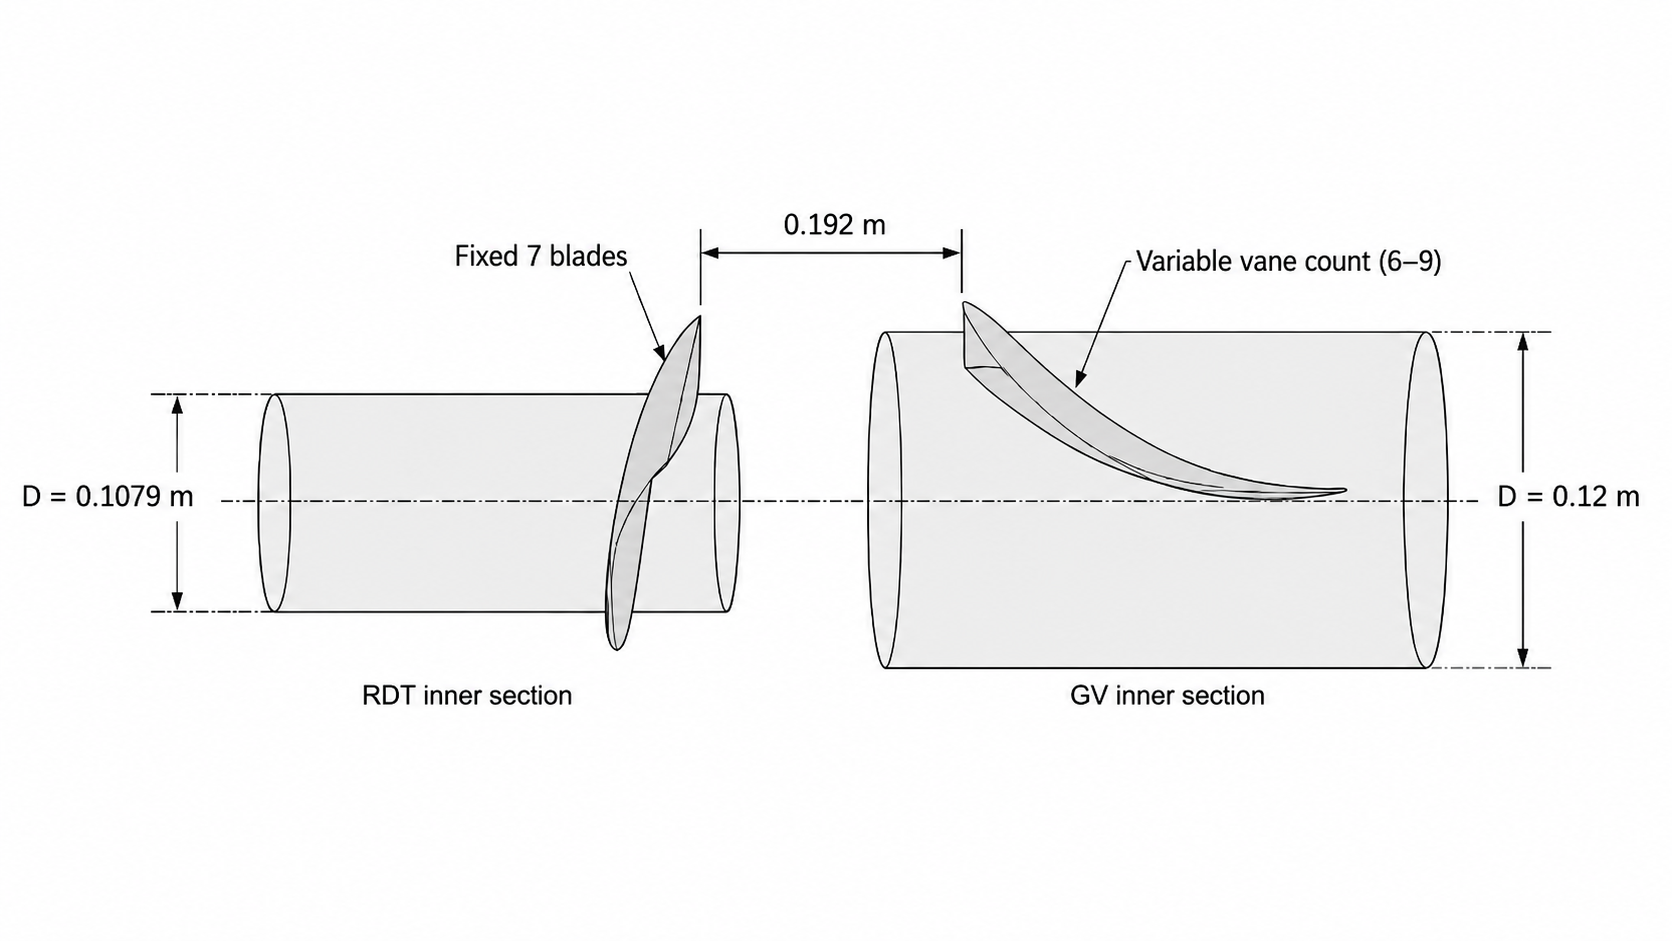
\includegraphics[width=0.95\textwidth]{Figures/2D_drawing/RDT-GV drawing.png}}
  \caption[Axial spacing between RDT and GV row]{Axial spacing between the RDT trailing edge and the guide-vane leading edge in the present configuration. The RDT has $Z_r = 7$ rotor blades fixed across the screening matrix, while the vane count $Z_s$ varies between 6 and 9 across the 18 GV configurations (Section~\ref{sec:methods_design_matrix}). The axial gap is $a = 0.192$~m.}
  \label{fig:rdt_gv_axial_spacing}
\end{figure}

\paragraph{Comparison with the G\"ulich compact-stage bound.}
The axial spacing is most informatively normalised by the impeller (rotor) chord $L$, following the convention of G\"ulich~\cite{Gulich2010} and Bijukchhe and Trivedi~\cite{Bijukchhe2026} discussed in Section~\ref{sec:rsi-axial-spacing}. The chord of the RDT blade varies along the span. Post-processing of the blade geometry of Djupesland and Trivedi~\cite{DjupeslandTrivedi2025} gives a chord of $L = 125.5$~mm at $r = 0.121$~m and $L = 197.0$~mm at $r = 0.232$~m. The span-averaged value across the nine radial sections that fall within the GV-overlap region $r \in [0.12, 0.25]$~m is $\bar{L} = 169.8$~mm. The corresponding spacing ratio is
\begin{equation}
    \frac{a}{\bar{L}} \;=\; \frac{0.192}{0.170} \;=\; 1.13,
    \label{eq:my_a_over_L}
\end{equation}
which exceeds the upper bound of the G\"ulich window $a/L = 0.05$-$0.15$ by a factor of $7.5$. The conclusion is robust to the choice of representative chord: even using the largest chord at the shroud ($L_{\max} = 197.0$~mm) gives $a/L = 0.97$, still $6.5$ times the upper limit. The bound~\eqref{eq:gulich_a_over_L} is therefore a qualitative reference for the importance of rotor-stator spacing, not a numerical design constraint that the present geometry should satisfy. Two consequences for the analysis follow.

\paragraph{Reduced potential interaction.}
The pressure field attached to each rotor blade decays approximately exponentially with axial distance from the rotor trailing edge~\cite{Korakianitis1989,Hodson1989}. With $a/\bar{L} = 1.13$, the potential-interaction component of the rotor-stator pulsation field reaching the GV leading edge is expected to be significantly weaker than in a compact stage. Two studies quantify the scaling. Rodriguez et al.~\cite{Rodriguez2007} observed $40$-$50\,\%$ pulsation amplitude reduction in the vaneless space when the rotor-stator gap was increased in a comparable pump-turbine geometry. Liu et al.~\cite{Liu2022GapMatching} confirmed this trend for multiphase pumps. This is consistent with one of the design objectives of the Store2Hydro layout: the GV row is intended primarily as a swirl-recovery element, not as a tightly coupled stator stage of the RDT.

\paragraph{Persistent viscous interaction.}
The viscous (wake) component is less attenuated by axial spacing. The RDT wake convects downstream through the gap, and the velocity-deficit and azimuthal-non-uniformity content reaches the GV leading edge largely intact~\cite{Korakianitis1989,Duan2019}. The transient simulations in Section~\ref{sec:monitor-setup} are interpreted in this light: the rotor-stator interaction signature in the spectra at $f_{\mathrm{BPF}}$ is expected to be dominated by viscous wake-chopping rather than potential interaction, with corresponding implications for the ring-coherence diagnostic in Section~\ref{sec:spec-coherence}.

A focused follow-up study that varies $a$ explicitly is identified as future work in Chapter~\ref{chap:future_work}.

\subsection{Boundary conditions}
\label{sec:methods_bc}
 
The boundary conditions used in all 18 configurations, in the \texttt{NoGV} reference and in the two transient diagnostic runs are summarised in Table~\ref{tab:bc_master}.
 
\begin{table}[h!]
  \centering
  \caption[Boundary conditions for the screening simulations]{Boundary conditions used in the 18-case screening campaign and the \texttt{NoGV} reference. The transient runs (\texttt{CC\_450\_7} and \texttt{CC\_400\_6}) use identical settings except that the rotor-stator interfaces are switched from frozen rotor to transient rotor-stator.}
  \label{tab:bc_master}
  \small
  \begin{tabular}{p{0.30\linewidth} p{0.62\linewidth}}
    \toprule
    \textbf{Boundary} & \textbf{Condition} \\
    \midrule
    Inlet (region 1, upstream face)
        & Total pressure $p_{\mathrm{tot}} = 101\,325$~Pa (1~atm),
          turbulence intensity $5\,\%$, axial inflow direction normal to face. \\
    Outlet (region 6, downstream face)
        & Mass flow rate $\dot m = 290.3$~kg/s. \\
    Walls (all regions, including RDT and GV blade surfaces)
        & Smooth no-slip, automatic wall treatment in the SST formulation. \\
    Reference pressure
        & $p_{\mathrm{ref}} = 0$~Pa (absolute pressure used throughout). \\
    Working fluid
        & Liquid water at $25^\circ$C, default ANSYS material properties. \\
    Rotor speed (region 2 only)
        & $n = 650$~rpm, axis aligned with the duct centreline. \\
    \midrule
    \multicolumn{2}{c}{\textbf{Interfaces}} \\
    \midrule
    Region 1 - Region 2
        & Stationary-rotating, frozen rotor (steady) or transient rotor-stator (transient run). \\
    Region 2 - Region 3
        & Rotating-stationary, frozen rotor (steady) or transient rotor-stator (transient run). \\
    Region 3 - Region 4
        & Stationary-stationary, GGI. \\
    Region 4 - Region 5
        & Stationary-stationary, GGI. \\
    Region 5 - Region 6
        & Stationary-stationary, GGI. \\
    \bottomrule
  \end{tabular}
\end{table}
 
\paragraph{Choice of total-pressure inlet.}
The inlet boundary condition is a total pressure rather than an imposed velocity profile. This choice is motivated by the fact that the inflow to the RDT in the laboratory is taken from a slow upstream reservoir-like region with very low dynamic head, so total pressure is well defined and approximately equal to atmospheric plus the small static head from the upstream tank. A velocity-profile inlet would require an additional simulation upstream of the RDT to produce a profile that is consistent with the inlet pipe length, which would introduce its own modelling assumptions. Using a total-pressure inlet leaves the velocity profile inside region 1 to develop naturally before reaching the RDT.
 
\paragraph{Choice of mass-flow outlet.}
The outlet specifies $\dot m = 290.3$~kg/s. Combined with the total-pressure inlet, this fixes the operating point uniquely while leaving the static pressure field free to develop. The chosen mass flow corresponds to the laboratory operating point that the Store2Hydro programme has adopted as the design point for the RDT booster~\cite{DjupeslandTrivedi2025, Fjuk2025}. Using a mass-flow outlet rather than a static-pressure outlet has the practical advantage that the operating point is enforced exactly across all 18 configurations, so that comparisons between cases are at strictly the same flow rate.
 
\paragraph{Rotational speed.}
The rotational speed $n = 650$~rpm is the design speed of the RDT booster in the parallel Store2Hydro work~\cite{DjupeslandTrivedi2025, Fjuk2025}. It gives the rotor frequency $f_n = 10.83$~Hz and the blade-passing frequency $f_{\mathrm{BPF}} = Z_r \cdot f_n = 75.83$~Hz used in the transient analysis (Section~\ref{sec:rsi-thesis}). All 18 steady configurations and the two transient runs are simulated at this speed. Off-design behaviour is not investigated and is identified as future work in Chapter~\ref{chap:future_work}.
 
% ---------------------------------------------------------------------
\section{Mesh strategy and grid convergence}
\label{sec:methods_mesh}

The mesh strategy is region-specific. The rotating RDT mesh and the guide-vane mesh are generated in ANSYS~TurboGrid because TurboGrid produces structured hexahedral O-grids with controlled $y^+$, low skewness and well-defined orthogonality on blade rows. The inner-pipe section $r < 0.12$~m for the guide-vane region is meshed with a structured-hub block. The remaining regions, namely the inlet pipe, the conical contraction, the $90^\circ$ bend and the final straight inlet pipe, are meshed in ANSYS~Meshing with unstructured tetrahedral elements and prismatic inflation layers near the walls. The discretisation uncertainty in the structured TurboGrid regions is assessed through bounded mesh-quality metrics, while the discretisation uncertainty in the unstructured draft-tube region is assessed through a full triplet-based Grid Convergence Index study following Celik et al.~\cite{Celik2008}. The reasons for this two-tier strategy are explained below.

\subsection{Rotor and guide-vane meshes (TurboGrid)}
\label{sec:turbogrid_quality}

Each of the 18 guide-vane configurations in Table~\ref{tab:design_matrix} is meshed independently in TurboGrid because chord and solidity differ between cases. The RDT rotor mesh is generated by the same workflow, using curve files exported from the upstream RDT design~\cite{DjupeslandTrivedi2025}. Refinement at the inner-pipe-to-blade transition resolves the boundary layer across the rotating-stationary interface. The targets applied to both the RDT and GV meshes are
\begin{itemize}
  \item $y^+ \approx 1$ on the vane surfaces (low-Reynolds wall treatment of SST $k$-$\omega$);
  \item minimum face angle $\geq 20^\circ$;
  \item maximum element expansion ratio $\leq 1.4$;
  \item minimum determinant $\geq 0.4$;
  \item element count per blade passage in the range $5\times 10^5$ - $1.5\times 10^6$, depending on chord.
\end{itemize}
TurboGrid reports these metrics directly for every generated mesh. Figure~\ref{fig:turbogrid_mesh} shows the TurboGrid mesh for one representative CC configuration and one representative CS configuration. The structured hexahedral O-grid wraps each blade in the cylindrical reference frame, and the boundary-layer cells on the suction surface reach the targeted $y^+ \approx 1$ resolution.

\begin{figure}[h!]
  \centering

  \begin{subfigure}[t]{0.48\textwidth}
    \centering
    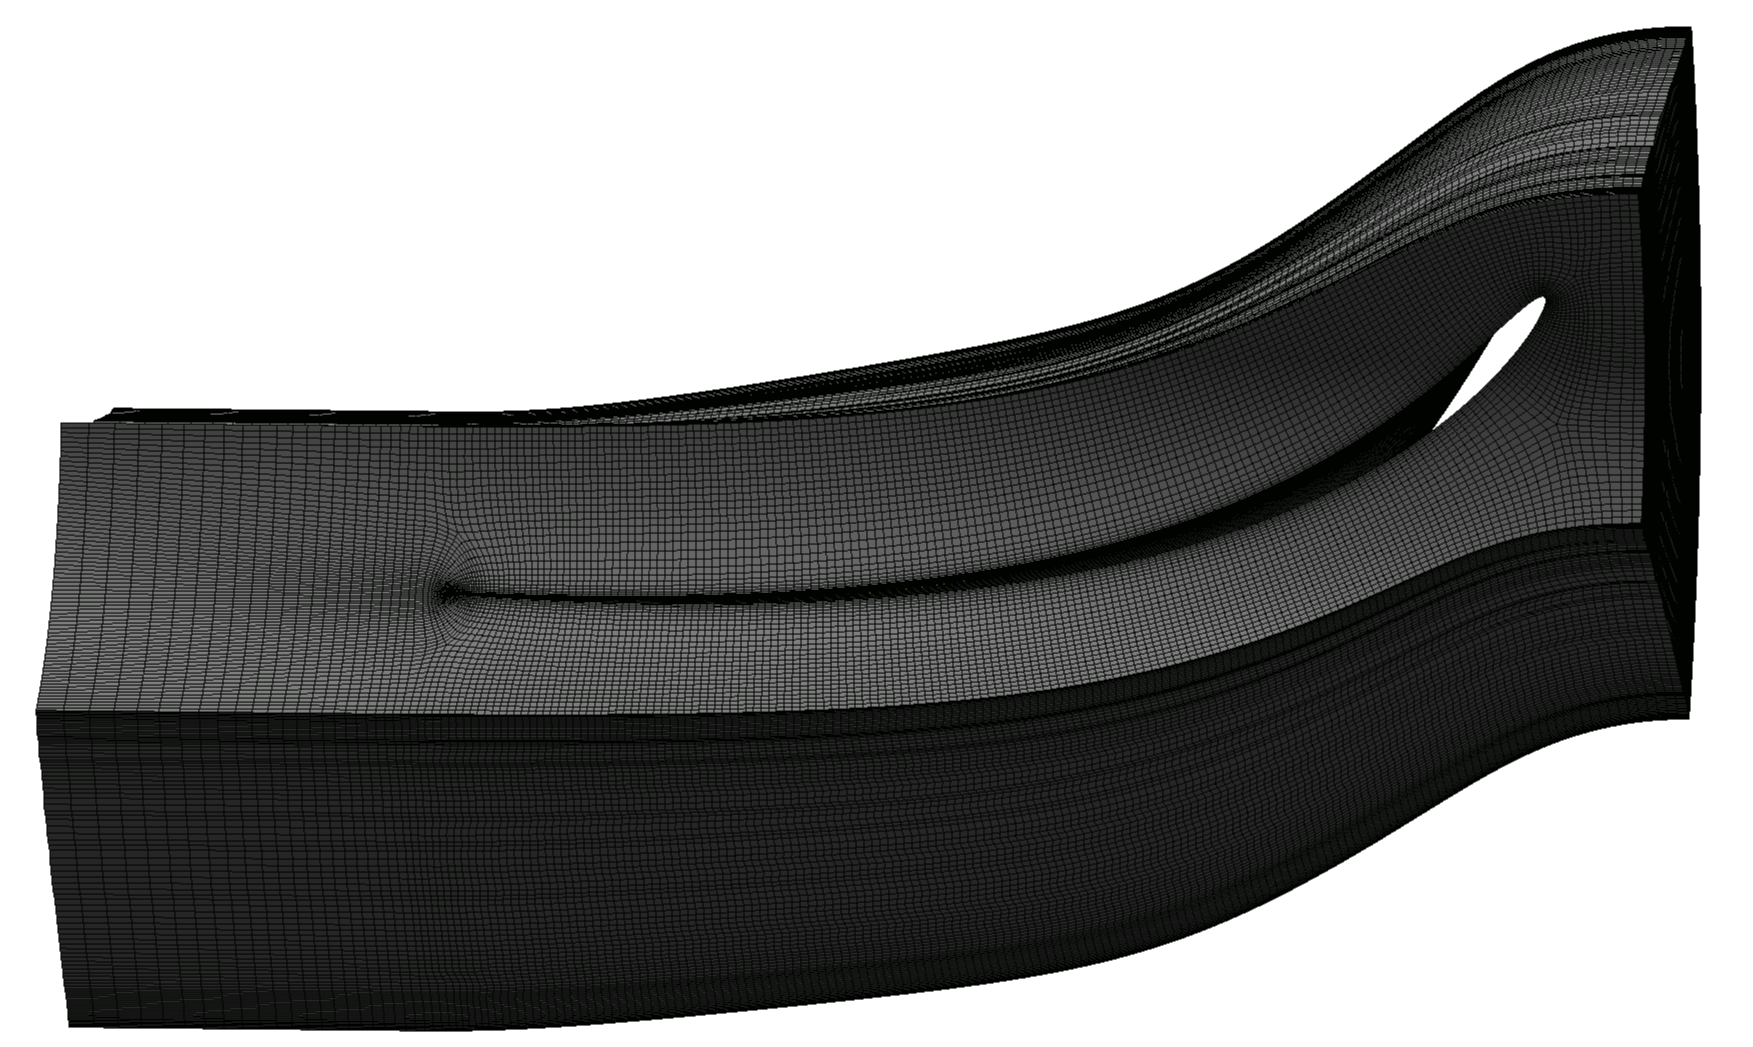
\includegraphics[width=\textwidth]{Figures/Mesh/Turbogrid_mesh2_CC.png}
    \caption{CC, view from hub.}
    \label{fig:turbogrid_cc_2}
  \end{subfigure}
  \hfill
  \begin{subfigure}[t]{0.48\textwidth}
    \centering
    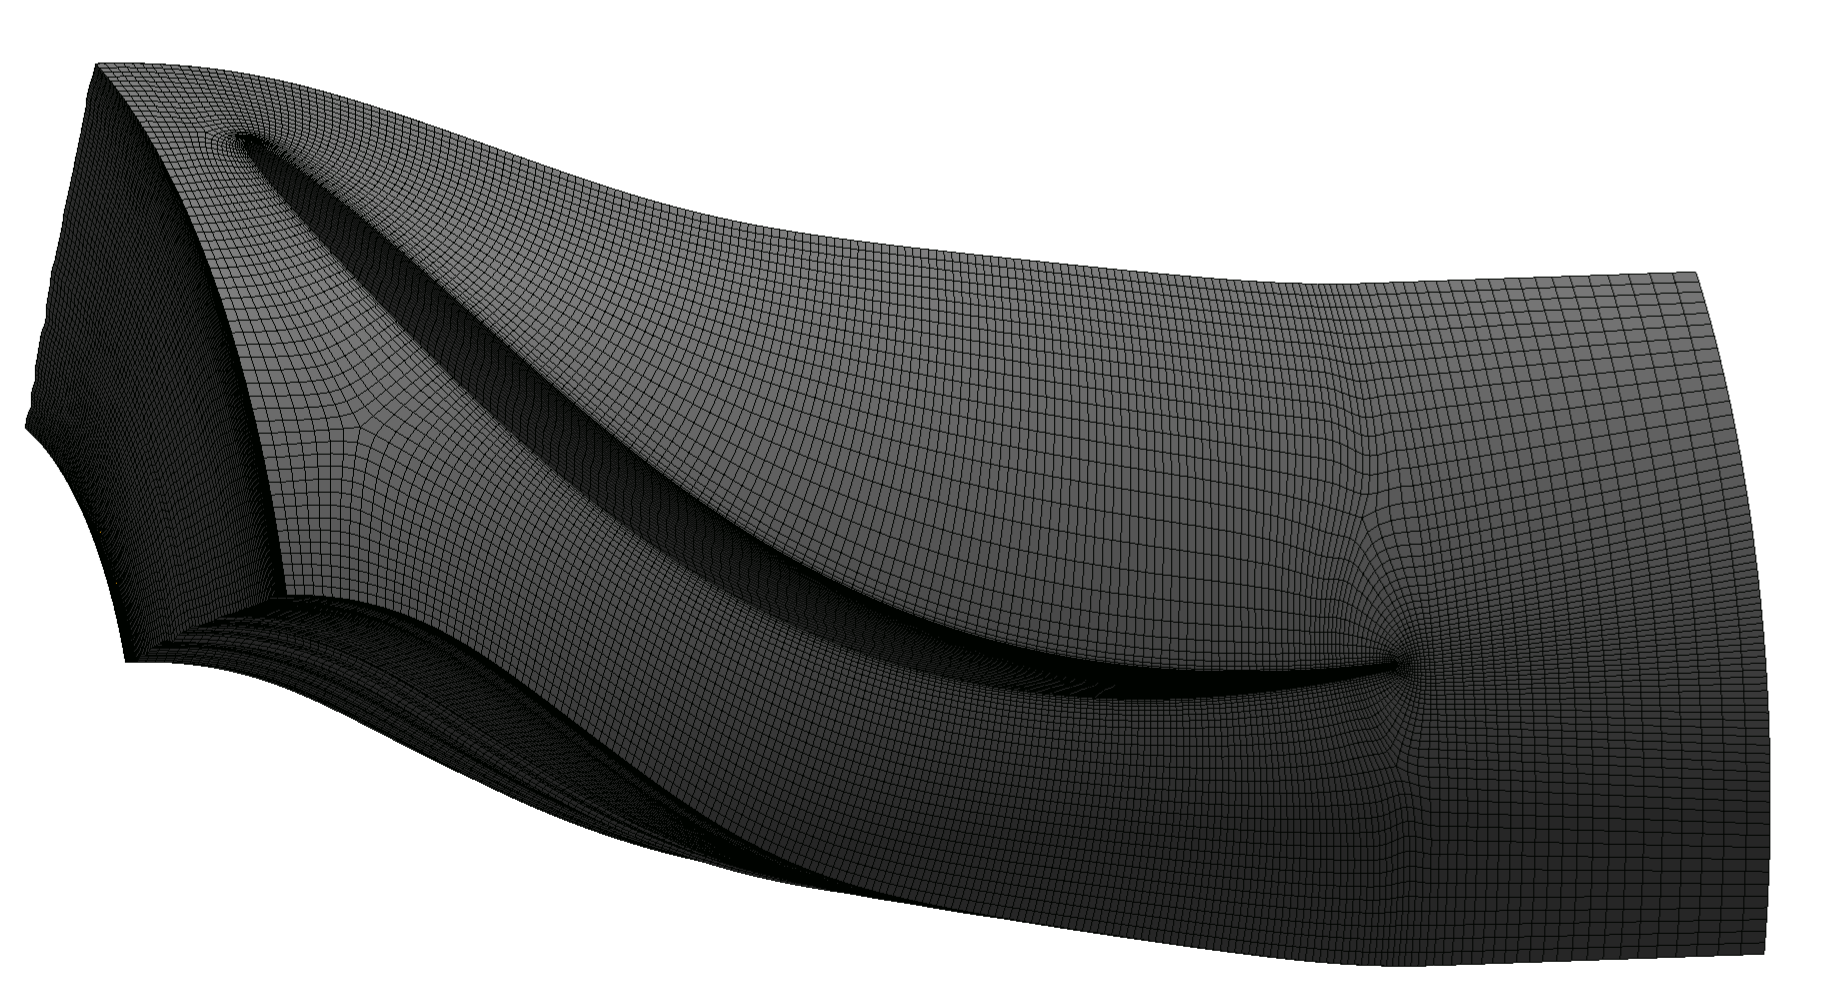
\includegraphics[width=\textwidth]{Figures/Mesh/Turbogrid_mesh3_CC.png}
    \caption{CC, view from shroud.}
    \label{fig:turbogrid_cc_3}
  \end{subfigure}

  \vspace{0.6em}

  \begin{subfigure}[t]{0.48\textwidth}
    \centering
    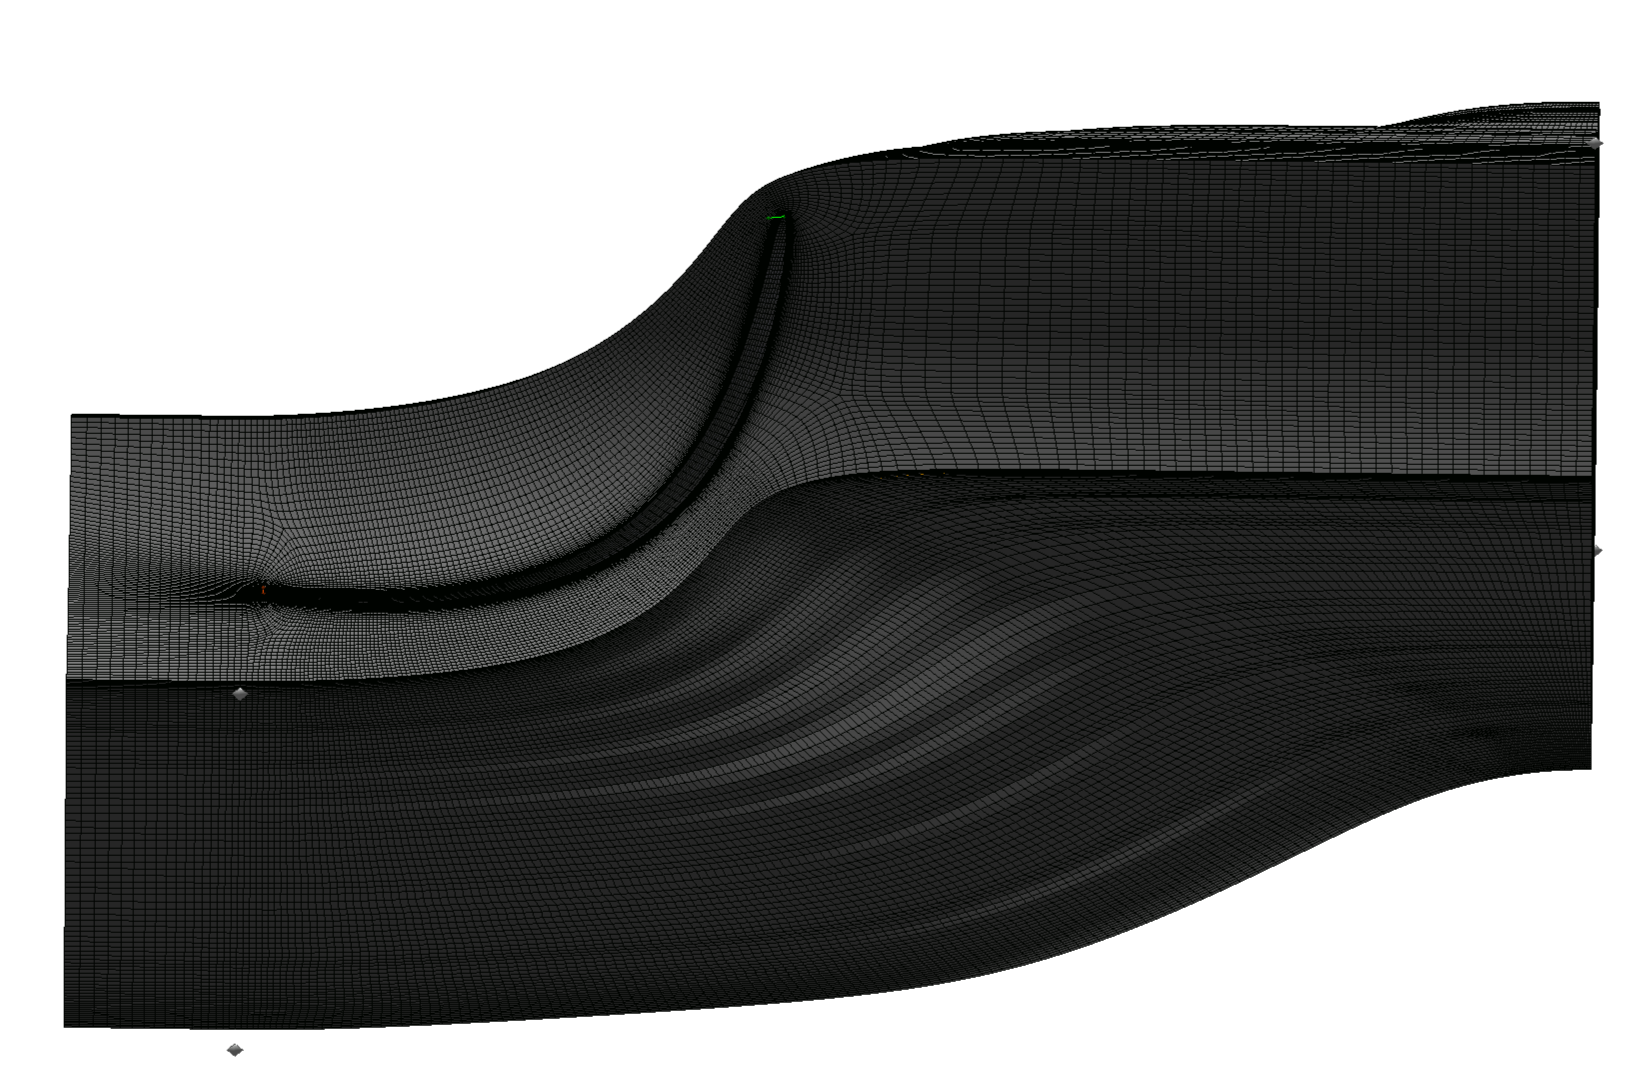
\includegraphics[width=\textwidth]{Figures/Mesh/Turbogrid_mesh2_CS.png}
    \caption{CS, view from hub.}
    \label{fig:turbogrid_cs_2}
  \end{subfigure}
  \hfill
  \begin{subfigure}[t]{0.48\textwidth}
    \centering
    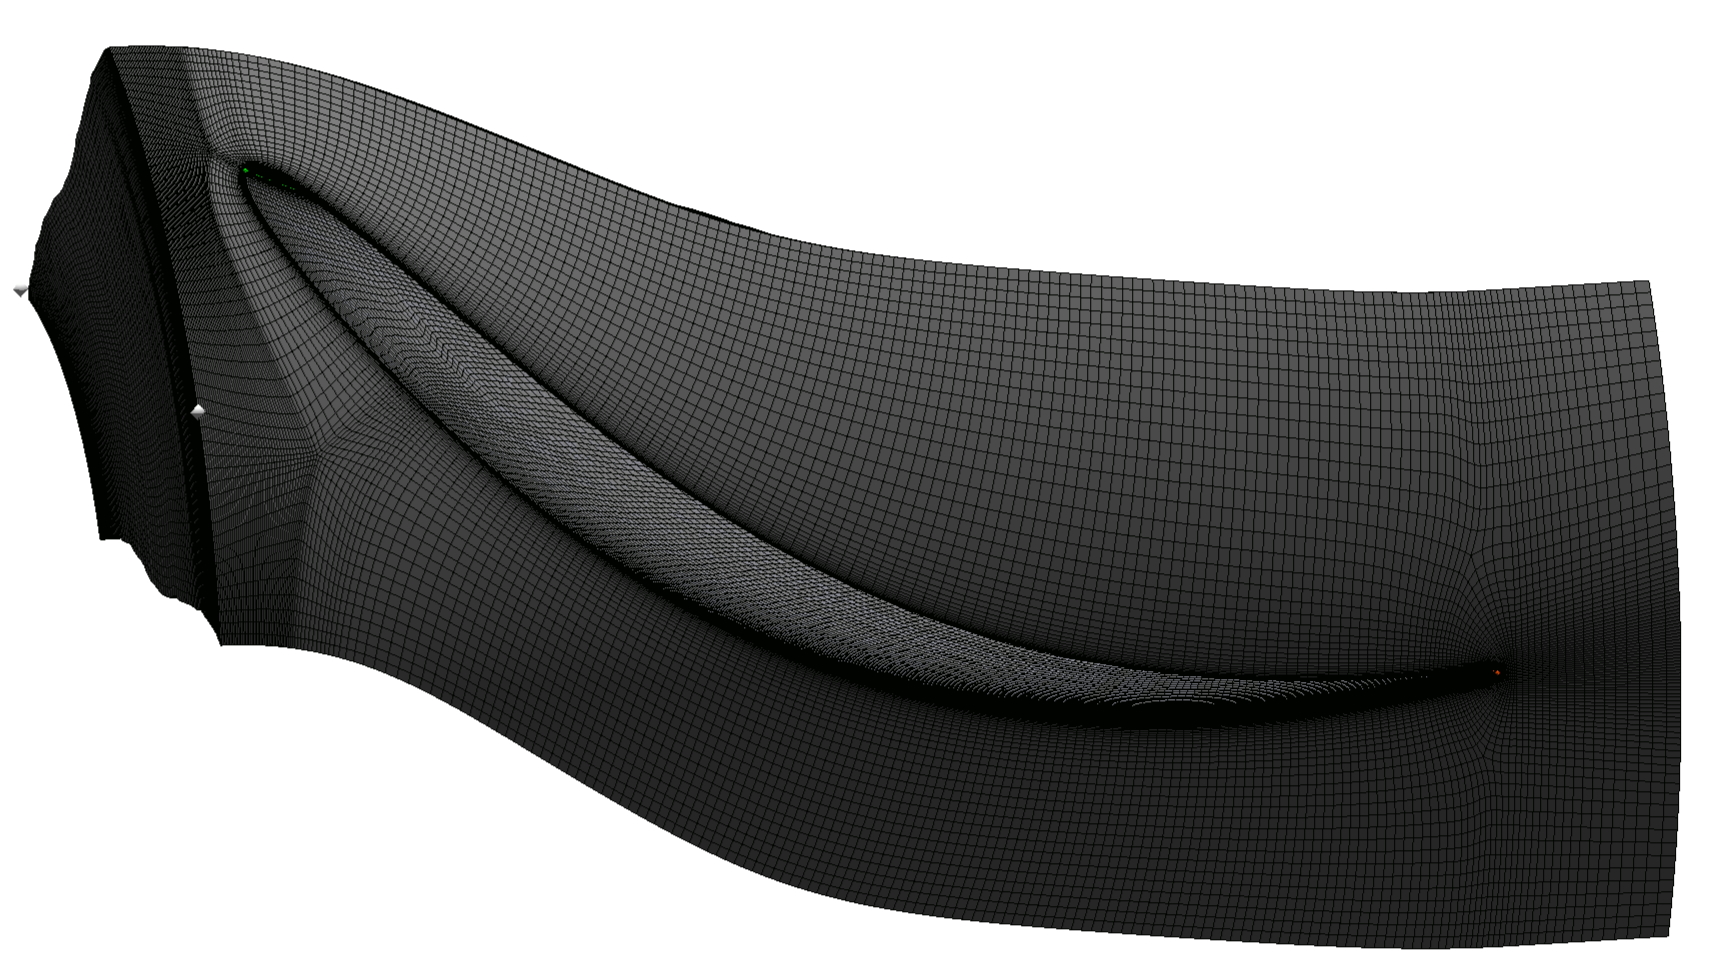
\includegraphics[width=\textwidth]{Figures/Mesh/Turbogrid_mesh3_CS.png}
    \caption{CS, view from shroud.}
    \label{fig:turbogrid_cs_3}
  \end{subfigure}

  \caption[GV TurboGrid mesh, CC and CS]{Representative TurboGrid mesh for one CC configuration (top row) and one CS configuration (bottom row).}
  \label{fig:turbogrid_mesh}
\end{figure}

\paragraph{Local orthogonality excursions in CS configurations.}
Some CS configurations produced local cells with orthogonality angles below the TurboGrid Min Limit of $20^\circ$, with the smallest values around $17^\circ$. The affected cells are localised in regions where the inlet-to-leading-edge distance varies along the span. This is intrinsic to the constant-solidity construction: the chord scales linearly with $r$, so the LE moves axially across the span and the upstream block becomes mildly skew. The fraction of affected cells is approximately $0.004\,\%$ of the global cell count. The expected impact on the integral output quantities is therefore negligible. The affected meshes are retained for the screening campaign on this basis. The remaining mesh-quality metrics (face angles, expansion ratio, determinant, skewness) satisfy the TurboGrid limits everywhere in the GV and RDT meshes.

A separate triplet-based GCI study is not performed for each blade row in the screening campaign. The reason is partly methodological and partly practical. Each guide-vane configuration in the screening matrix has its own chord, solidity and twist distribution. TurboGrid generates a fresh structured topology for every case, so a single triplet of refinement levels does not transfer between configurations. A separate triplet study would have to be repeated 18 times. The methodological justification is that the SST $k$-$\omega$ model with $y^+ \approx 1$ has well-established mesh-independence properties on a structured hexahedral O-grid with bounded skewness and aspect ratio~\cite{Menter1994}. Once the bounds above are met, the integral output quantities of interest (head loss across the vane row, integrated tangential force, swirl-number reduction) are mesh-independent. The discretisation uncertainty in the rotor and stator blade meshes is therefore assessed indirectly through the bounded mesh-quality metrics rather than through a full GCI procedure.

\subsection{Inflation layers and $y^+$ targets}
\label{sec:methods_inflation}

The inflation layers in the unstructured regions (inlet pipe, cone, bend, final pipe) target $30 \leq y^+ \leq 80$ on the pipe walls, consistent with the logarithmic-layer assumption of the SST automatic wall treatment. On the rotating RDT blades and on the guide-vane surfaces, the structured TurboGrid mesh targets $y^+ \leq 1$, so that the SST low-Reynolds branch is active near the wall. The number of inflation layers is set to 15 with a growth ratio of approximately $1.2$, which is sufficient to resolve the boundary layer at the design Reynolds number. The mesh-quality targets and the discretisation-assessment method for the three regions are summarised in Table~\ref{tab:mesh_quality}.

\begin{table}[h!]
\centering
\caption[Mesh-quality summary across the three computational regions]{Mesh-quality targets and assessment method for the three computational regions. The structured blade meshes are assessed through bounded mesh-quality metrics (this section). The unstructured draft-tube mesh is assessed through the triplet-based GCI procedure of Section~\ref{sec:gci_drafttube}.}
\label{tab:mesh_quality}
\small
\begin{tabular}{l c c c}
\toprule
                            & RDT rotor       & GV row                                   & Draft tube \\
                            & (TurboGrid)     & (TurboGrid)                              & (unstructured) \\
\midrule
Element type                & Hex (O-grid)    & Hex (O-grid)                             & Tet + prism \\
$y^+$ on walls              & $\approx 1$    & $\approx 1$                              & $30$-$80$ \\
Min face angle              & $\geq 20^\circ$ & $\geq 20^\circ$ (CS: $17^\circ$ locally) & - \\
Max expansion ratio         & $\leq 1.4$     & $\leq 1.4$                               & - \\
Min determinant             & $\geq 0.4$     & $\geq 0.4$                               & - \\
Inflation layers            & -             & -                                      & 15, growth $\sim 1.2$ \\
Discretisation assessment   & Bounded metrics & Bounded metrics                          & GCI (Sec.~\ref{sec:gci_drafttube}) \\
\bottomrule
\end{tabular}
\end{table}

\subsection{Draft-tube mesh and the GCI procedure}
\label{sec:gci_drafttube}

The draft-tube domain (regions 5 and 6) contains the conical contraction, the $90^\circ$ bend and the final straight inlet pipe. This is the part of the domain where the result is most sensitive to mesh resolution. The bend produces secondary flow with cross-stream gradients that can be substantially under-resolved if the cross-stream cell density is low. The post-bend axial-velocity profile drives several of the post-processing metrics, including the residual swirl at ConeEnd and the post-bend total-pressure loss. A formal Grid Convergence Index study is therefore carried out for the draft-tube domain following the procedure of Celik et al.~\cite{Celik2008}, with the safety factor $F_s = 1.25$ recommended for three-mesh studies in the same reference.

The procedure uses three meshes related by an effective refinement ratio $r > 1.3$,
\begin{equation}
h_i \;=\; \!\left(\frac{1}{N_i}\right)^{1/3}, \qquad
r_{21} = h_2 / h_1, \quad r_{32} = h_3 / h_2,
\label{eq:GCI_h_r}
\end{equation}
where $N_i$ is the number of cells on grid $i$ (1 = fine, 2 = medium, 3 = coarse). The apparent order of convergence is estimated by fixed-point iteration of
\begin{equation}
p \;=\; \frac{1}{\ln r_{21}} \,\Bigl|\,\ln\!\bigl|(\phi_3 - \phi_2)/(\phi_2 - \phi_1)\bigr|\,\Bigr|,
\label{eq:GCI_p}
\end{equation}
and the Richardson-extrapolated value follows from
\begin{equation}
\phi_{\mathrm{ext}} \;=\; \phi_1 + \frac{\phi_1 - \phi_2}{r_{21}^{\,p} - 1}.
\label{eq:GCI_extrap}
\end{equation}
The reported uncertainty on the medium-to-fine pair is
\begin{equation}
\mathrm{GCI}_{12} \;=\; F_s\,\frac{\bigl|\phi_2 - \phi_1\bigr|}{\bigl|\phi_1\bigr|\,(r_{21}^{\,p} - 1)} \times 100\,\%, \qquad F_s = 1.25,
\label{eq:GCI_def}
\end{equation}
and the same expression is used for $\mathrm{GCI}_{23}$ on the coarse-to-medium pair. The acceptance target adopted for every quantity used as a ranking metric is $\mathrm{GCI}_{12} \leq 2\,\%$. This is tighter than the $\mathrm{GCI}_{12} \leq 3\,\%$ commonly adopted for industrial CFD~\cite{Celik2008}. It is consistent with the values obtained by Jenssen~\cite{Jenssen2020} on the related RPT domain in this project.

\paragraph{Mesh triplet.}
Three meshes were generated for the draft-tube domain by uniform refinement of a common base topology. Cell counts and refinement ratios are reported in Table~\ref{tab:gci_meshes}; both ratios exceed the lower bound of $1.3$ recommended by Celik et al.~\cite{Celik2008}. The three meshes are visualised in Figure~\ref{fig:gci_meshes}.

\begin{table}[h!]
  \centering
  \caption[Mesh triplet for the GCI study]{Cell counts and refinement ratios for the GCI study on the draft-tube domain. Refinement is performed in three spatial dimensions, $h_i = (1/N_i)^{1/3}$.}
  \label{tab:gci_meshes}
  \small
  \begin{tabular}{l r r}
    \toprule
    \textbf{Mesh}  & \textbf{Cell count $N$}  & \textbf{Refinement ratio} \\
    \midrule
    Coarse ($N_3$) & $2\,313\,100$            & $r_{32} = 1.289$ \\
    Medium ($N_2$) & $4\,956\,300$            & $r_{21} = 1.305$ \\
    Fine   ($N_1$) & $11\,003\,000$           & - \\
    \bottomrule
  \end{tabular}
\end{table}

\begin{figure}[h!]
  \centering
  \begin{subfigure}[t]{0.32\textwidth}
    \centering
    \includegraphics[width=\textwidth]{Figures/Mesh/Mesh_DT_Coarse_cross.png}
    \caption{Coarse, $N_3 = 2.31\times 10^6$ cells.}
    \label{fig:gci_mesh_coarse}
  \end{subfigure}
  \hfill
  \begin{subfigure}[t]{0.32\textwidth}
    \centering
    \includegraphics[width=\textwidth]{Figures/Mesh/Mesh_DT_Medium_cross.png}
    \caption{Medium, $N_2 = 4.96\times 10^6$ cells.}
    \label{fig:gci_mesh_medium}
  \end{subfigure}
  \hfill
  \begin{subfigure}[t]{0.32\textwidth}
    \centering
    \includegraphics[width=\textwidth]{Figures/Mesh/Mesh_DT_Fine_cross.png}
    \caption{Fine, $N_1 = 11.00\times 10^6$ cells.}
    \label{fig:gci_mesh_fine}
  \end{subfigure}
  \caption[Draft-tube meshes used in the GCI study]{Cross-sections of the three draft-tube meshes used in the GCI study. The base topology is preserved across the triplet so that the refinement is uniform in all three spatial dimensions.}
  \label{fig:gci_meshes}
\end{figure}

\paragraph{Two reference configurations.}
The GCI is evaluated for two configurations on the same draft-tube domain. The first is a \emph{straight-flow} verification case in which the RDT rotor is removed and a uniform axial velocity is prescribed at the inlet; this configuration has no physical swirl and serves as a numerical-noise reference. The second is the \emph{swirling-flow} operational case with the RDT active, which is the configuration relevant to the screening campaign. Running both configurations on the same triplet separates two distinct error sources. The first is numerical generation of spurious tangential motion in regions where the cross-stream cell density is insufficient to resolve the bend curvature, which is visible only in the straight-flow case because the underlying physical answer there is zero. The second is the finite-grid resolution of the genuine swirling-flow gradients, which is visible in the swirling-flow case. The post-processing planes are those defined in Section~\ref{sec:methods_planes_metrics}; the same surface positions are evaluated in both configurations. The plane layout on the swirling-flow solution is shown in Figure~\ref{fig:planes_overview}.

A total of seventy integral output quantities are extracted on these planes for both configurations: mass-flow-averaged total pressure $\overline{p_t}^{\,m}$ and total head $\Delta H_{\mathrm{tot}}$, area-averaged static pressure $\overline{p}^{\,a}$, mean flow angle $\overline{\alpha}^{\,m}$, area-averaged swirling strength, and the design-span-restricted swirl number $S$ defined in Section~\ref{sec:methods_planes_metrics}.

\subsection{Straight-flow configuration: spurious-swirl signature}
\label{sec:gci_straight}

The most informative quantity in the straight-flow configuration is the mean flow angle. By symmetry, an axisymmetric uniform-inflow configuration through an axisymmetric duct should yield $\alpha = 0^\circ$ on every analysis plane. Any non-zero value is therefore a purely numerical artefact and represents discretisation-induced spurious tangential motion generated when the cross-stream cell density in the bend cannot fully resolve the secondary-flow curvature term. Selected values are summarised in Table~\ref{tab:gci_straight_keep}.

\begin{table}[h!]
  \centering
  \caption[GCI - straight-flow configuration]{Selected GCI results for the straight-flow configuration (RDT removed, uniform axial inlet). Spurious tangential motion is the dominant numerical artefact and is largest on the coarse mesh. Pressure and total-head quantities are insensitive to it.}
  \label{tab:gci_straight_keep}
  \small
  \begin{tabular}{l r r r r r}
    \toprule
    \textbf{Quantity}                            & \textbf{Fine} & \textbf{Medium} & \textbf{Coarse} & $\mathbf{GCI_{12}}$ & $\mathbf{GCI_{23}}$ \\
    \midrule
    Angle ConeEnd  $[\,^\circ\,]$                & $6.556$       & $6.779$         & $6.950$         & $6.06\,\%$  & $4.76\,\%$  \\
    Angle GVEnd4   $[\,^\circ\,]$                & $1.238$       & $1.230$         & $1.220$         & $2.55\,\%$  & $3.38\,\%$  \\
    Angle GVStart  $[\,^\circ\,]$                & $0.054$       & $0.048$         & $0.047$         & $19.79\,\%$ & $3.93\,\%$  \\
    \midrule
    Tot.\ Pressure GVEnd     $[\mathrm{Pa}]$     & $102\,400$    & $102\,409$      & $102\,423$      & $0.02\,\%$  & $0.03\,\%$  \\
    Tot.\ Pressure BendEnd   $[\mathrm{Pa}]$     & $102\,287$    & $102\,303$      & $102\,318$      & $0.03\,\%$  & $0.03\,\%$  \\
    Tot.\ Head GVEnd $[\mathrm{m}]$              & $10.470$      & $10.471$        & $10.472$        & $0.25\,\%$  & $0.26\,\%$  \\
    Static Pressure ConeEnd $[\mathrm{Pa}]$      & $99\,359$     & $99\,377$       & $99\,397$       & $0.14\,\%$  & $0.16\,\%$  \\
    \bottomrule
  \end{tabular}
\end{table}

The coarse mesh produces a non-physical mean flow angle of $6.95^\circ$ at ConeEnd. This decreases monotonically to $6.78^\circ$ on the medium mesh and $6.56^\circ$ on the fine mesh, with $\mathrm{GCI}_{12} = 6.06\,\%$ and $\mathrm{GCI}_{23} = 4.76\,\%$. The same signature is seen at GVStart with $\mathrm{GCI}_{12} = 19.79\,\%$, although in absolute terms the angle remains below $0.06^\circ$ on all three meshes. The integrated pressure and total-head quantities are insensitive to the artefact: the kinetic-energy contribution of a sub-degree spurious angle is negligible, and Table~\ref{tab:gci_straight_keep} confirms that all such quantities have $\mathrm{GCI}_{12} < 0.3\,\%$ already on the medium mesh. The straight-flow configuration therefore identifies the coarse mesh as inadequate for the present geometry: it generates a measurable numerical swirl in a configuration where the physical answer is zero.

\subsection{Swirling-flow configuration: the two quantities that exceed the threshold}
\label{sec:gci_swirl}

In the swirling-flow configuration, 65 of the 70 monitored quantities meet the $\mathrm{GCI}_{12} \leq 2\,\%$ acceptance criterion on the medium mesh. The accepted set includes all primary ranking metrics for the screening campaign: total head $\Delta H_{\mathrm{tot}}$ and mass-flow-averaged total pressure on the GVEnd-series, BendStart and BendEnd planes; static pressure on the same planes; the mean flow angle at ConeEnd; and the donut-restricted swirl number $S$ at the GVEnd, GVEnd6 and BendEnd planes. The corresponding $\mathrm{GCI}_{12}$ values lie in the range $0.05\,\%$-$0.6\,\%$ across all primary ranking metrics. Rather than reproducing the full table for these well-converged quantities, the present subsection focuses on a small set of quantities. For these the medium mesh is converged with respect to the fine mesh, while the coarse mesh is \emph{not} converged with respect to the medium mesh. This is the direction of error that is most informative for the choice of working mesh and is reported in Table~\ref{tab:gci_swirl_keep}.

\begin{table}[h!]
  \centering
  \caption[GCI - swirling-flow configuration: quantities exceeding the $2\,\%$ threshold]{The two integral quantities in the swirling-flow configuration that satisfy $\mathrm{GCI}_{12} < 2\,\%$ together with $\mathrm{GCI}_{23} > 2\,\%$. The medium mesh has reached the asymptotic range with respect to the fine mesh, while the coarse mesh has not reached the asymptotic range with respect to the medium mesh. The two quantities are the area-averaged swirling strength immediately upstream of the guide-vane row, and the donut-restricted swirl number on the first post-vane plane downstream of the row.}
  \label{tab:gci_swirl_keep}
  \small
  \begin{tabular}{l r r r r r}
    \toprule
    \textbf{Quantity}                                            & \textbf{Fine}  & \textbf{Medium} & \textbf{Coarse} & $\mathbf{GCI_{12}}$ & $\mathbf{GCI_{23}}$ \\
    \midrule
    Swirling strength upstream of GV $[\mathrm{s}^{-1}]$         & $32.952$       & $32.484$        & $33.645$        & $1.14\,\%$ & $\mathbf{3.08\,\%}$ \\
    Swirl number $S$ downstream of GV (donut)                    & $2.420$        & $2.412$         & $2.422$         & $1.61\,\%$ & $\mathbf{2.12\,\%}$ \\
    \bottomrule
  \end{tabular}
\end{table}

Both quantities are evaluated in regions with the steepest cross-stream gradients in the domain. The first is the immediate near-wake of the rotating RDT, the second is the first post-vane plane. The largest sensitivity to mesh density is physically expected here. This is the textbook signature of a mesh that has just entered the asymptotic range. The medium mesh has converged with respect to the fine mesh, but the coarse mesh has not converged with respect to the medium mesh. The medium mesh is therefore acceptable; the coarse mesh is not. The same direction of error, $\mathrm{GCI}_{23} > \mathrm{GCI}_{12}$, is observed in most of the swirl-related quantities throughout the swirl-dominated region. This holds even where the magnitudes of both indices remain below $2\,\%$, and confirms that the coarse-to-medium error is systematically larger than the medium-to-fine error.

\paragraph{Note on the RDT torque.}
The integrated torque on the RDT is the only quantity in the swirling-flow configuration with $\mathrm{GCI}_{12}$ above $2\,\%$ on the medium-to-fine pair. This is consistent with the verification work of Dokset~\cite{Dokset2025} on the same domain. The steady frozen-rotor formulation of the rotor-stator interface used here is known not to deliver torque values in the asymptotic mesh-convergence range. The interface only enforces a fixed relative position between the rotor and the stator and does not capture the physical unsteadiness of the rotor-stator interaction. Torque is therefore not used as a ranking metric in the present screening, in agreement with the approach taken by Dokset~\cite{Dokset2025} for the same domain.

\subsection{Selection of the working mesh}
\label{sec:gci_pick}

Three lines of evidence support the selection of the medium mesh as the working mesh for the screening campaign.

The first is the spurious-swirl test in the straight-flow configuration. The coarse mesh produces a non-physical mean flow angle of $6.95^\circ$ at ConeEnd in a configuration that should yield zero by construction (Table~\ref{tab:gci_straight_keep}). The medium mesh reduces this artefact to within $0.22^\circ$ of the fine-mesh value. The screening campaign is built around the analysis of swirl-related quantities downstream of the guide vanes. A mesh that introduces about $7^\circ$ of artificial swirl in a swirl-free configuration cannot be trusted to represent the genuine swirl in the operational configuration. The coarse mesh is rejected on this test alone.

The second is the convergence behaviour on the swirling-flow ranking metrics. Of the seventy monitored quantities in the swirling-flow configuration, sixty-five satisfy $\mathrm{GCI}_{12} \leq 2\,\%$ on the medium mesh, with most values in the range $0.1\,\%$-$0.6\,\%$. The two quantities that do not satisfy the criterion together with $\mathrm{GCI}_{23} \leq 2\,\%$ are the swirling strength upstream of the guide vanes and the swirl number on the first post-vane plane (Table~\ref{tab:gci_swirl_keep}). Both have $\mathrm{GCI}_{12} < 2\,\%$ on the medium mesh, and exceed the threshold only on the coarse mesh. The medium mesh therefore lies within the asymptotic range with respect to the fine mesh on every quantity used in the design ranking, while the coarse mesh does not reach the asymptotic range on the most sensitive swirl-related quantities. This is the direct quantitative argument for the medium mesh: the coarse mesh fails the convergence test where it matters most, and the medium mesh passes it.

The third is the cost ratio. The fine mesh has $2.22\times$ the cell count of the medium mesh and a corresponding increase in solve time. For an 18-case screening campaign, this cost is not justified by the additional accuracy on the ranking metrics. The medium-to-fine differences on $\Delta H_{\mathrm{tot}}$, total pressure and the swirl number lie below the design separation between the screening configurations. The screening ranking is therefore preserved when the medium mesh is used in place of the fine mesh. The same trade-off was made by Jenssen~\cite{Jenssen2020} on the related RPT domain, who selected the medium mesh on the grounds that the increase in computational cost from medium to fine was not worth the improvement in discretisation error.

The medium mesh of $4.96\times 10^6$ cells is therefore adopted for the RDT, draft-tube and downstream-duct regions in all 18 configurations of the screening campaign and in the two transient diagnostic runs. The coarse mesh is retained only for the present GCI study and is not used in any of the production simulations.

\paragraph{Note on coverage.}
The GCI study reported above covers the unstructured draft-tube region, which includes the conical contraction, the bend and the final straight pipe. The structured TurboGrid blade meshes are not included, for the reasons given in Section~\ref{sec:turbogrid_quality}. The combined two-tier strategy gives a defensible picture of the discretisation uncertainty. It uses a Celik~\cite{Celik2008} GCI on the unstructured draft-tube domain together with bounded TurboGrid quality metrics on the 18 structured blade meshes. It avoids the additional computing time that 18 separate triplet-based GCI studies on the rotating and stator blade rows would require.
 
% ---------------------------------------------------------------------
\section{Solver settings and convergence}
\label{sec:methods_solver}
 
ANSYS~CFX is used as the solver throughout. The numerical settings adopted for the steady screening campaign are summarised in Table~\ref{tab:cfx_settings_master}.
 
\begin{table}[h!]
  \centering
  \caption[Solver settings, screening campaign]{Numerical settings used in the steady-state screening campaign.}
  \label{tab:cfx_settings_master}
  \small
  \begin{tabular}{l l}
    \toprule
    \textbf{Setting} & \textbf{Value} \\
    \midrule
    Solver                       & ANSYS CFX, steady RANS, incompressible \\
    Turbulence model             & SST $k$-$\omega$ \\
    Advection scheme             & High Resolution \\
    Turbulence numerics          & First Order\\
    Timescale control            & Auto (physical timescale derived from rotor speed) \\
    Convergence target           & RMS residuals $\leq 10^{-5}$ for momentum and continuity \\
    Mass-imbalance target        & $|\dot m_{\mathrm{out}} - \dot m_{\mathrm{in}}|/\dot m_{\mathrm{in}} \leq 0.1\,\%$ \\
    Monitor stability            & Drift in monitor metrics $\leq 0.5\,\%$ over the last 200 iterations \\
    \bottomrule
  \end{tabular}
\end{table}
 
\paragraph{Operational notes from the campaign.}
Residual targets were achieved for all 18 configurations, but the swirl reduction at the post-vane planes was less aggressive than in the project-work simple-pipe simulations~\cite{Leonsen2025}. Three factors contribute: the absence of the RPT suction field; the cumulative redistribution by the conical contraction and the bend; and the fixed conservative slip correction $\delta_{\mathrm{TE}} = 6^\circ$ (Section~\ref{sec:theory_incidence_deviation}). The interpretation in Chapter~\ref{chap:results_discussion} compares all 18 cases against the no-GV reference to keep the ranking meaningful even though the absolute swirl reduction is smaller than in the simpler project-work geometry.
 
% ---------------------------------------------------------------------
\section{Analysis planes and post-processing metrics}
\label{sec:methods_planes_metrics}
 
A common array of analysis planes is defined for every configuration so that all 18 cases and the \texttt{NoGV} reference can be compared on identical cross-sections. The plane positions are summarised in Table~\ref{tab:planes}, listed in the streamwise order from the RDT to the RPT inlet.
 
\begin{table}[h!]
  \centering
  \caption[Analysis planes]{Common array of analysis planes used in the post-processing of all 18 configurations and the \texttt{NoGV} reference.}
  \label{tab:planes}
  \small
  \begin{tabular}{l|l}
    \toprule
    \textbf{Plane label} & \textbf{Position} \\
    \midrule
    RDTStart   & RDT leading-edge plane \\
    RDT        & RDT trailing-edge plane \\
    LE         & Guide-vane leading-edge plane \\
    GVStart    & Same as LE, used for diagnostic redundancy \\
    GVEnd      & Guide-vane trailing-edge plane \\
    GVEnd2 \dots GVEnd6 & Series of post-vane planes at increasing axial distance \\
    ConeEnd    & End of the conical contraction \\
    BendStart  & Start of the $90^\circ$ bend \\
    BendEnd    & End of the $90^\circ$ bend \\
    \bottomrule
  \end{tabular}
\end{table}

\begin{figure}[h!]
  \centering
  \includegraphics[width=0.85\textwidth]{Figures/Mesh/GCI_planes.png}
  \caption[Common array of analysis planes]{Common array of analysis planes used in the post-processing of all 18 configurations, the \texttt{NoGV} reference and the GCI study, shown on a swirling-flow solution. Plane labels follow Table~\ref{tab:planes}; the GVEnd-series (GVEnd2 to GVEnd6) is distributed along the conical contraction. Plane normals are aligned with the local duct centreline.}
  \label{fig:planes_overview}
\end{figure}
 
On each plane, the following metrics are extracted using mass-flow-averaged or area-averaged operators in CFX-Post:
\begin{itemize}
  \item static and total pressure $\overline{p}$, $\overline{p_t}$, both mass-flow-averaged and area-averaged;
  \item total head $H = \overline{p_t}/(\rho g)$;
  \item swirl number $S$ (Eq.~\ref{eq:S_def}) and its design-span-restricted version $S_{\mathrm{span}}$ over the design span $r \in [0.12, 0.25]$;
  \item area-averaged swirling strength $\overline{\lambda_{ci}}$;
  \item turbulent kinetic energy $\overline{\mathrm{TKE}}$ and its plane maximum;
  \item mass-flow-averaged flow angle $\overline{\alpha}^{m}$.
\end{itemize}
Mass-flow conservation between consecutive planes is checked separately as a sanity test. Forces and torques on the rotor and on a representative guide vane are extracted in addition.
 
\paragraph{Composite ranking metric.}
For preliminary screening only, a composite ranking metric is defined as
\begin{equation}
J \;=\; w_1\,\widehat{\Delta H}_{\mathrm{tot}} + w_2\,\widehat{|S|}_{\mathrm{ConeEnd}} + w_3\,\widehat{\mathrm{UI}}_{\mathrm{ax,ConeEnd}},
\label{eq:composite}
\end{equation}
where each hat denotes the corresponding metric normalised between the worst and the best values across the 18 configurations, and the weights $\{w_1, w_2, w_3\} = \{0.45, 0.35, 0.20\}$ reflect a moderate preference for low loss while still penalising poor swirl recovery. The composite is used as a screening shortcut and is not the basis for the final ranking. The final ranking is based on the Pareto-front analysis between $\Delta H_{\mathrm{tot}}$ and $|S|_{\mathrm{ConeEnd}}$, supported by the spanwise diagnostics on the shortlisted configurations.
 
% ---------------------------------------------------------------------
\section{No-GV reference simulation}
\label{sec:methods_rdt_baseline}
 
A reference simulation of the same domain with the guide vanes \emph{removed}, denoted \texttt{NoGV} in Table~\ref{tab:design_matrix}, is performed to provide the baseline against which all 18 configurations are compared. In this reference, region 3 is replaced by an empty straight pipe of equal length while every other aspect of the domain, the boundary conditions and the solver settings is held identical. The simulation produces the no-GV residual swirl in the draft-tube section, which is used to normalise the swirl-reduction metric:
\begin{equation}
\mathcal{R}_S(\mathrm{plane}) \;=\; \frac{S_{\mathrm{NoGV}}(\mathrm{plane}) - S_{\mathrm{case}}(\mathrm{plane})}{S_{\mathrm{NoGV}}(\mathrm{plane})}.
\label{eq:swirl_reduction}
\end{equation}
The \texttt{NoGV} reference is also used to verify that the RDT model produces the expected wake structure (high swirl concentrated in the outer span, low-momentum or back-flow region in the centre, swirling-strength concentrated in the tip-vortex helix). Visual inspection of the reference confirms the qualitatively correct behaviour, which gives confidence that the inflow to the guide-vane region is dominated by the RDT in the way that the project work~\cite{Leonsen2025} designed for. In addition, the $\Delta H$ between the same plane pair in \texttt{NoGV} and in each case quantifies how much of the total pressure loss comes from the guide vanes themselves, rather than from the upstream RDT or the downstream duct.
 
% ---------------------------------------------------------------------
\section{Justification for not coupling with the RPT}
\label{sec:rpt-decoupling-justification}
 
The decision to replace the RPT by a $\sim 1.0$~m extended straight pipe is the most consequential simplification in the present setup. It is justified by three considerations, all of which are specific to the master-thesis context.
 
\paragraph{Computational budget.} A coupled RDT-GV-RPT simulation in CFX requires about $3$-$4$ times more wall-clock time per case than the present RDT-GV-draft-tube simulation. Three factors drive this. The RPT runner adds a rotating-mesh region. The runner blades require smaller blade-passage cell sizes. The rotor-stator interfaces require stricter timescale control for stable convergence. With 18 configurations to simulate, the available computational allocation does not accommodate this scaling.
 
\paragraph{Division of work in the Store2Hydro programme.} The parallel master thesis by Dokset~\cite{Dokset2025} is dedicated to the RPT-side analysis and to the cavitation behaviour of the runner under various pre-rotation conditions imposed at the runner inlet. The work is therefore divided between the two theses. The present thesis screens the guide-vane design space and identifies a small number of candidate configurations that produce favourable inflow conditions at the bend exit. Dokset's thesis takes selected inflow profiles, including those produced by the present screening, and assesses the resulting pump-mode performance and cavitation margin in the RPT. A coupled simulation by either side would duplicate the other side's responsibility.
 
\paragraph{Comparability of the relative ranking.} The screening question is a relative one: which of the 18 configurations is most favourable on the recovery-loss trade-off? The relative ranking is preserved when the missing RPT suction field acts approximately uniformly across the cases, to first order in the differences between them. The cases share downstream geometry and operating point, so this holds. Absolute values of head loss and residual swirl will shift when the RPT is reintroduced; the ranking is expected to be less sensitive.
 
A coupled simulation of the selected configuration (the case identified by the Pareto analysis as the recommended candidate) with the RPT included is identified in Chapter~\ref{chap:future_work} as the natural follow-up to this work and is left as future work.
 
% ---------------------------------------------------------------------
\section{Method limitations}
\label{sec:methods_limitations_master}
 
Even within the well-defined screening scope of this thesis, several limitations should be stated honestly:
\begin{itemize}
  \item \textbf{Single inlet wake.} All 18 configurations are designed against the same RDT wake. The screening therefore reflects the relative behaviour of the configurations under the specific inflow used, and the ranking may shift with a different RDT design or operating point.
  \item \textbf{Single operating point.} Only the nominal $\dot m = 290.3$~kg/s, $n = 650$~rpm condition is simulated. Off-design behaviour is not investigated.
  \item \textbf{Steady RANS.} Steady RANS is used for the screening. Two separate transient simulations (\texttt{CC\_450\_7} and \texttt{CC\_400\_6}) are performed for the rotor-stator interaction analysis but are not part of the main screening ranking.
  \item \textbf{No multiphase cavitation modelling.} Cavitation is treated indirectly through the static-pressure field; vapour-fraction modelling is not performed in the screening campaign.
  \item \textbf{No coupled RPT.} The RPT is replaced by an extended straight pipe, as discussed in Section~\ref{sec:rpt-decoupling-justification}.
  \item \textbf{No structural assessment.} Strength, fatigue and vibration of the guide vanes are not analysed in the screening campaign.
  \item \textbf{Slip correction held fixed.} The slip-correction value is held fixed at $\delta_{\mathrm{TE}} = 6^\circ$ across all 18 configurations rather than swept, in line with the discussion in Section~\ref{sec:theory_incidence_deviation}.
\end{itemize}

% ---------------------------------------------------------------------
\section{Transient simulation setup and monitor points}
\label{sec:monitor-setup}
 
Two transient simulations are run in addition to the steady screening campaign. The first is \texttt{CC\_450\_7}, the project-work baseline with $Z_r=Z_s=7$ and the $m_{\min}=0$ reference. The second is \texttt{CC\_400\_6}, the $m_{\min}\geq 1$ counterpart from the screening matrix. The choice of \texttt{CC\_400\_6} rather than \texttt{CC\_450\_6} is motivated in Section~\ref{sec:rsi-thesis}. Both runs are performed in ANSYS~CFX at $n = 650$~rpm to assess the unsteady loading at the nominal operating point and to provide the time histories needed for the spectral analysis. The interface between the rotating RDT domain and the stationary GV domain is specified as a Transient Rotor-Stator (TRS) interface; all other solver settings follow those established for the steady screening campaign (Section~\ref{sec:methods_solver}).
 
The time step is fixed at $\Delta t = T_{\mathrm{rev}}/360 = 2.564\times 10^{-4}$~s, corresponding to one degree of rotor rotation per time step. The total simulated physical time is $15\,T_{\mathrm{rev}} \approx 1.38$~s, allowing the initial transient to decay over approximately ten rotor revolutions before the last five revolutions are retained for Fourier analysis.
 
\subsection{Coordinate system and reference positions}
\label{sec:coord-system}
 
The coordinate system used throughout the spectral analysis has its origin at the geometric centre of the RDT hub, with the positive $z$-axis pointing downstream towards the RPT. The RDT blade volume occupies $-0.185~\mathrm{m} \leq z \leq +0.185~\mathrm{m}$, so that the RDT-GV interface plane is located at
\begin{equation}
    z_{\mathrm{ref}} \;=\; -0.185~\mathrm{m}. \label{eq:zref}
\end{equation}
The duct radius is $R = 0.25$~m, consistent with the baseline geometry established in~\cite{Leonsen2025}. Downstream of $z_{\mathrm{ref}}$ there is a short unloaded transition before the GV leading edge, and the GV domain extends to $z = -0.685$~m, giving a total GV domain length of 500~mm.
 
Axial monitor positions are hereafter reported as the distance downstream of the RDT-GV interface,
\begin{equation}
    s \;=\; |z| - |z_{\mathrm{ref}}|,
    \qquad 0~\mathrm{mm} \leq s \leq 500~\mathrm{mm},
\end{equation}
which is more convenient for physical interpretation than absolute $z$-coordinates because $s$ counts from a physically meaningful plane (the rotor-stator interface) rather than from the RDT hub centre.
 
\subsection{Monitor-signal indexing}
\label{sec:monitor-index}
 
Seven monitor signals are exported from the CFX solver manager and used in the spectral analysis. To keep figure axis labels and table rows compact, each signal is assigned a short label in Table~\ref{tab:monitor-index}. These short labels are used on all figures in Chapter~\ref{chap:results_discussion} and in Appendix~\ref{app:individual_spectra}; their full meaning is to be read from Table~\ref{tab:monitor-index}.
 
\begin{table}[H]
\centering
\small
\caption{Indexing of monitor signals used in the FFT analysis. The short label is used on all plots. Positions refer to the coordinate system defined in Section~\ref{sec:coord-system} ($s$ measured from the RDT-GV interface at $z_{\mathrm{ref}} = -0.185$~m).}
\label{tab:monitor-index}
\begin{tabular}{p{0.12\textwidth} p{0.20\textwidth} p{0.36\textwidth} p{0.24\textwidth}}
\hline
Label & Quantity & Location / averaging & CFX expression \\ \hline
\multicolumn{4}{l}{\textit{Group A - force on a single guide vane (GV1)}} \\
$F_{\mathrm{res}}$ & Resultant force & Integrated on GV1 surface & \texttt{Fres GV1} \\[0.4em]

\multicolumn{4}{l}{\textit{Group B - torque on the rotor}} \\
$M_{\mathrm{RDT}}$ & Torque about rotation axis & Integrated over full RDT & \texttt{torque\_z()@Entire BLADE} \\[0.4em]

\multicolumn{4}{l}{\textit{Group C - plane-averaged pressures}} \\
$P_{\mathrm{in}}$ & Static pressure, mass-flow avg. & Plane at $s = 0$ mm (RDT-GV interface) & \texttt{massFlowAve(p)@RDT\_GV} \\
$P_{\mathrm{out}}$ & Static pressure, mass-flow avg. & Plane at $s = 500$ mm (GV outlet) & \texttt{massFlowAve(p)@GV\_DT} \\[0.4em]

\multicolumn{4}{l}{\textit{Group D - wall-pressure probes at $r/R = 0.744$ along the GV passage}} \\
$P_0$ & Static pressure & $s = 0$ mm, $r/R = 0.744$ (near GV leading edge) & \texttt{Static Pressure point} \\
$P_3$ & Static pressure & $s = 300$ mm, $r/R = 0.744$ (inside GV passage) & \texttt{Static Pressure point} \\
$P_5$ & Static pressure & $s = 500$ mm, $r/R = 0.744$ (at GV outlet) & \texttt{Static Pressure point} \\ \hline
\end{tabular}
\end{table}
 
\paragraph{Groups of purpose.}
The signals fall into four functional groups:
\begin{itemize}
  \item \emph{Group A - Force on a single guide vane.} The resultant force $F_{\mathrm{res}}$ on a representative guide vane (GV1) is the principal diagnostic for cyclic structural loading.
  \item \emph{Group B - Torque on the rotor.} $M_{\mathrm{RDT}}$ is the torque about the rotation axis integrated over the entire RDT blade set and captures periodic torque ripple from rotor-stator interaction.
  \item \emph{Group C - Plane-averaged pressures.} Two mass-flow-averaged plane signals, $P_{\mathrm{in}}$ at the RDT-GV interface and $P_{\mathrm{out}}$ at the GV outlet, extract the axisymmetric $m=0$ component of the pulsation field. Comparison of $P_{\mathrm{in}}$ and $P_{\mathrm{out}}$ amplitudes quantifies how much of the coherent $m=0$ content is attenuated across the GV row.
  \item \emph{Group D - Wall-pressure probes along the GV passage.} Three probes $P_0$, $P_3$, $P_5$ at the fixed radial position $r/R = 0.744$ along one azimuthal line sample the full pulsation field, including the spinning modes $|m|\geq 1$ that are washed out in the plane-averaged signals. In combination with $P_{\mathrm{out}}$ they permit the ring-coherence diagnostic defined in Eq.~\eqref{eq:coherence}.
\end{itemize}
 
\section{Spectral analysis methodology}
\label{sec:spec}
 
The force, torque and pressure signals from the monitors described in Section~\ref{sec:monitor-index} are analysed in the frequency domain using the discrete Fourier transform. This section summarises the sampling, window and amplitude-calibration relations and defines the ring-coherence diagnostic used to classify the dominant spatial mode of the pulsation field.
 
\subsection{Discrete Fourier transform and sampling}
\label{sec:spec-dft}
 
A monitor signal $x(t)$ is recorded at the transient solver time step $\Delta t$, giving $N$ uniformly spaced samples $x_n = x(n\Delta t)$, $n = 0,1,\dots,N-1$. The sampling frequency and Nyquist frequency are
\begin{equation}
    f_s \;=\; \frac{1}{\Delta t},\qquad
    f_{\mathrm{Nyq}} \;=\; \frac{f_s}{2}. \label{eq:fs_fnyq}
\end{equation}
The discrete Fourier transform and frequency grid are
\begin{align}
    X_k &\;=\; \sum_{n=0}^{N-1} x_n\, e^{-i\,2\pi k n / N},
    \qquad k = 0,1,\dots,N-1, \label{eq:dft}\\
    f_k &\;=\; \frac{k}{N\Delta t} \;=\; k\,\Delta f,
    \qquad \Delta f = \frac{1}{N\,\Delta t} = \frac{f_s}{N}.
    \label{eq:dft_f}
\end{align}
To place the excitation frequencies $f_n$ and $f_{\mathrm{BPF}}$ exactly on Fourier bins and thereby minimise spectral leakage, the analysis window is chosen as an integer number of rotor revolutions,
\begin{equation}
    T_w \;=\; N_{\mathrm{rev}}\,T_{\mathrm{rev}},
    \qquad T_{\mathrm{rev}} = 1/f_n, \label{eq:Tw}
\end{equation}
so that $N = 360\,N_{\mathrm{rev}}$ at one degree of rotor rotation per solver step. With $N_{\mathrm{rev}}=5$ this gives $\Delta f = f_n/5$, i.e.\ five Fourier bins per rotor-frequency harmonic and 35 bins per blade passing harmonic.
 
\subsection{Hanning window and leakage correction}
\label{sec:spec-window}
 
Residual non-periodicity at the boundaries of the analysis window introduces spectral leakage from dominant peaks into neighbouring bins. Following standard practice for pressure-pulsation analysis in hydraulic turbomachinery~\cite{Kerlefsen2025,Bergan2018} the signal is multiplied by a Hanning window prior to the Fourier transform:
\begin{equation}
    w_n \;=\; \tfrac{1}{2}\!\left[ 1 - \cos\!\left(\tfrac{2\pi n}{N-1}\right)\right],
    \qquad n = 0,1,\dots,N-1. \label{eq:hanning}
\end{equation}
The mean is removed before windowing ($x'_n = x_n - \bar{x}$, $x^{w}_n = x'_n w_n$). The Hanning window reduces the effective signal energy by a factor $\sum_n w_n / N = 1/2$, so an amplitude correction is applied to recover the true peak amplitude. The single-sided amplitude spectrum used throughout this thesis is
\begin{equation}
    A_k \;=\; \frac{2}{\displaystyle\sum_{n=0}^{N-1} w_n}\,
      \bigl|X^{w}_k\bigr|,
    \qquad k = 0,1,\dots,\tfrac{N}{2}, \label{eq:amplitude}
\end{equation}
where the factor $2$ accounts for folding of negative frequencies onto the single-sided representation. $A_k$ has the same physical units as $x_n$ and represents the peak amplitude of a pure sinusoid at frequency $f_k$.
 
\subsection{Periodicity verification}
\label{sec:spec-periodicity}
 
The Fourier amplitudes $A_k$ are only meaningful if the underlying signal is statistically stationary over the analysis window. Two verifications are therefore performed:
\begin{enumerate}
  \item \emph{Phase-folded comparison.} The $N_{\mathrm{rev}}$ revolutions contained in the window are plotted on a common $[0,\,360^\circ]$ phase axis. A signal dominated by harmonics of $f_n$ produces nearly overlapping curves; deviation is a direct indicator of content at frequencies below $f_n$ or of incomplete transient decay.
  \item \emph{Window robustness test.} The spectrum is computed for $N_{\mathrm{rev}} = 5$ and $N_{\mathrm{rev}} = 6$ and the two spectra are overlaid. Stability of the peak amplitudes under variation of the window length confirms that the reported amplitudes are not an artefact of the particular window.
\end{enumerate}
 
\subsection{Ring-coherence diagnostic}
\label{sec:spec-coherence}
 
The Tyler-Sofrin analysis in Section~\ref{sec:rsi-tyler} distinguishes between the axisymmetric $m=0$ mode and the spinning modes with $|m|\geq 1$. Only the $m=0$ component produces a net axial force on the GV ring and propagates as a plane wave, whereas the spinning modes cancel in circumferential integration.
 
To classify the dominant spatial mode of the computed pulsation field without a full modal decomposition, a scalar ring-coherence diagnostic is defined. Let $A_{\mathrm{loc}}(f)$ denote the Fourier amplitude of a local wall-pressure signal (one of $P_0 \ldots P_5$) and $A_{\mathrm{ring}}(f)$ the amplitude of the plane-averaged signal $P_{\mathrm{out}}$ on the downstream plane. Because mass-flow averaging extracts the $m=0$ component of the field, $A_{\mathrm{ring}}$ measures the axisymmetric plane-wave content alone. The ring-coherence ratio is defined as
\begin{equation}
    \mathcal{R}_m(f) \;=\;
    \frac{A_{\mathrm{ring}}(f)}{A_{\mathrm{loc}}(f)},
    \qquad 0 \leq \mathcal{R}_m(f) \leq 1. \label{eq:coherence}
\end{equation}
Two limiting interpretations follow:
\begin{itemize}
  \item $\mathcal{R}_m(f_{\mathrm{BPF}}) \to 1$ indicates that the pulsation at $f_{\mathrm{BPF}}$ is dominated by the $m=0$ breathing mode. For $Z_r = Z_s$ this is the expected signature of the classical rotor-stator concern, and is the main signal that the \texttt{CC\_450\_7} transient run is designed to test.
  \item $\mathcal{R}_m(f_{\mathrm{BPF}}) \ll 1$ indicates that the pulsation is dominated by spinning modes $|m|\geq 1$ that cancel in circumferential integration. The net axial ring force is then small and the classical $Z_r = Z_s$ concern does not manifest strongly in practice. The \texttt{CC\_400\_6} transient run is the comparator from the screening matrix that is expected to display this behaviour.
\end{itemize}
 
\subsection{Characteristic excitation frequencies}
\label{sec:spec-peaks}
 
Table~\ref{tab:characteristic_freqs} lists the characteristic excitation frequencies for the two transient runs at $n = 650$~rpm. Note that $f_{\mathrm{BPF}}$ depends only on the rotor blade count $Z_r=7$ and is therefore the same for both \texttt{CC\_450\_7} and \texttt{CC\_400\_6}, while the vane passing frequency differs ($Z_s=7$ versus $Z_s=6$).
 
\begin{table}[H]
\centering
\caption{Characteristic excitation frequencies for the two transient runs ($n = 650$~rpm, $Z_r=7$).}
\label{tab:characteristic_freqs}
\begin{tabular}{lcccc}
\hline
 & Symbol & Formula & \texttt{CC\_450\_7} [Hz] & \texttt{CC\_400\_6} [Hz] \\ \hline
Rotor frequency           & $f_n$               & $n/60$         & 10.83  & 10.83  \\
Second rotor harmonic     & $2f_n$              & $2n/60$        & 21.67  & 21.67  \\
Third rotor harmonic      & $3f_n$              & $3n/60$        & 32.50  & 32.50  \\
Blade passing frequency   & $f_{\mathrm{BPF}}$  & $Z_r\,f_n$     & 75.83  & 75.83  \\
Vane passing frequency    & $f_{\mathrm{VPF}}$  & $Z_s\,f_n$     & 75.83  & 65.00  \\
Second BPF harmonic       & $2f_{\mathrm{BPF}}$ & $2Z_r\,f_n$    & 151.67 & 151.67 \\
Third BPF harmonic        & $3f_{\mathrm{BPF}}$ & $3Z_r\,f_n$    & 227.50 & 227.50 \\ \hline
\end{tabular}
\end{table}
 
A characteristic signature of rotor-stator interaction would be dominant peaks at $f_{\mathrm{BPF}}$ and its harmonics. Dominant energy at $f_n$ and its harmonics, in contrast, is typically associated with a once-per-revolution forcing such as a rotor imbalance, blade-to-blade variation in loading, or azimuthally non-uniform inflow into the RDT~\cite{Brekke2015,Bergan2018}. Both types of content are analysed in Chapter~\ref{chap:results_discussion}.

% ---------------------------------------------------------------------
\section{Velocity-triangle characterisation of the RDT wake}
\label{sec:methods_rdt_velocity_triangles}
 
The \texttt{NoGV} reference solution introduced above is also the source of the spanwise inflow field that drives every guide-vane configuration in the screening campaign. To document the wake that the guide vanes are designed against, the absolute velocity components $C_m$ and $C_u$ are extracted from the converged baseline solution at six radial spans: $r/R \in \{0.01,\,0.20,\,0.40,\,0.60,\,0.80,\,0.99\}$. Here $R$ is the normalised distance from hub to shroud, with $R_{\mathrm{hub}}=53.95$~mm and $R_{\mathrm{shroud}}=250.0$~mm. The values are sampled along blade-loading lines on the rotor blade at constant span. They are exported as $(s,\,V_{\mathrm{axial}})$ and $(s,\,V_{\mathrm{circ}})$. The coordinate $s\in[0,1]$ is the blade chordwise coordinate from the leading edge (LE, $s=0$) to the trailing edge (TE, $s=1$).
 
\paragraph{Sign convention.}
The CFD domain is oriented so that the bulk flow proceeds in the $-z$ direction and the rotor angular-velocity vector $\vec{\omega}$ is aligned with $z$; the rotor turns clockwise when viewed in the streamwise direction. ANSYS~CFX reports the axial and circumferential velocity components in a right-handed reference frame about $+z$. To produce quantities that follow the standard turbomachinery convention, where $C_m>0$ corresponds to streamwise flow and $C_u>0$ to motion in the rotor direction, the raw exports are sign-flipped:
\begin{equation}
C_m \;=\; -V_{\mathrm{axial},\mathrm{CFX}}, \qquad
C_u \;=\; -V_{\mathrm{circ},\mathrm{CFX}}, \qquad
U(r) \;=\; \omega\,r,
\label{eq:rdt_sign_convention}
\end{equation}
which yields the relative tangential component $W_u = C_u - U$ and the magnitudes $|\vec{C}|=\sqrt{C_m^{2}+C_u^{2}}$ and $|\vec{W}|=\sqrt{C_m^{2}+W_u^{2}}$. The radial component $C_r$ is neglected at this stage in line with the design assumption of Section~\ref{sec:theory_kinematics}.
 
\paragraph{Pressure-side and suction-side branches.}
A blade-loading line traces the rotor blade contour and therefore contains, at every streamwise position $s$, two velocity values that bracket the local through-flow: a pressure-side (PS) branch and a suction-side (SS) branch. The streamwise coordinate is binned into 200 equal intervals across $[0,1]$. For each bin the highest and lowest values delineate the PS-SS spread, while the bin mean provides a single representative line. This procedure is robust to scatter in the raw point cloud and does not require manual selection of individual blade-passage points.
 
\paragraph{Sampling regions.}
Two regions of the blade-loading line are post-processed and reported here. The trailing-edge region $s\in(0.90,\,1.00)$ is the most defensible proxy for the free-stream wake because the PS and SS branches converge towards a common value as the blade boundary layers merge into the wake. Values from this region are used as the spanwise design input $(\,r,\,C_m,\,C_u\,)$ passed to the guide-vane generator of Leonsen~\cite{Leonsen2025}. The near-leading-edge region $s\in[0.05,\,0.15]$ is reported as a complementary diagnostic of the local kinematics on the suction surface immediately downstream of the LE stagnation and suction-peak region. The near-LE values are not free-stream inlet velocities to the rotor, and they are not used as design input; they document the kinematic state of the flow on the blade surface in the high-incidence region near the LE.
 
\paragraph{Trailing-edge values used as guide-vane design input.}
The TE values obtained from the procedure above are summarised in Table~\ref{tab:rdt_te_values} and visualised in Figure~\ref{fig:rdt_velocity_triangles_TE}. They are subsequently passed to the guide-vane generator as the three spanwise input vectors \texttt{r\_span}, \texttt{Cm\_span} and \texttt{Cu\_span}. The corresponding absolute flow angle at the guide-vane leading edge,
\begin{equation}
\alpha(r) \;=\; \arctan\!\left(\frac{C_u(r)}{C_m(r)}\right),
\label{eq:alpha_definition}
\end{equation}
is the quantity that the design code internally evaluates as the inlet-flow angle and uses to set the leading-edge metal angle $\theta_1(r)=-\alpha(r)$, that is, zero incidence to the incoming absolute flow~\cite{Leonsen2025}. $\alpha(r)$ is the absolute flow angle relevant to a stationary vane row. The relative angle $\beta(r)=\arctan(W_u/C_m)$ is reported in the same table for completeness but is not used to design the stationary guide vanes.
 
\begin{table}[H]
  \centering
  \caption[RDT trailing-edge velocity triangle at six spans]{Velocity triangle components at the RDT trailing edge ($s>0.90$) for the six selected spans, used as the spanwise design input for every configuration in the screening campaign. $\alpha$ is the absolute flow angle defined in \eqref{eq:alpha_definition} and is the quantity the guide-vane generator uses to set the LE metal angle. All values follow the sign convention of \eqref{eq:rdt_sign_convention}.}
  \label{tab:rdt_te_values}
  \begin{tabular}{ccccccccc}
    \hline
    span & $r$ & $U$ & $C_m$ & $C_u$ & $W_u$ & $|\vec{C}|$ & $\alpha$ & $\beta$ \\
         & [mm] & [m/s] & [m/s] & [m/s] & [m/s] & [m/s] & [$^\circ$] & [$^\circ$] \\
    \hline
    0.01 &  55.9 &  3.81 & 0.67 &  3.57 & $-0.24$ &  3.63 & $+79.3$ & $-19.7$ \\
    0.20 &  93.2 &  6.34 & 1.41 &  4.62 & $-1.72$ &  4.83 & $+73.0$ & $-50.6$ \\
    0.40 & 132.4 &  9.01 & 1.31 &  6.76 & $-2.25$ &  6.88 & $+79.0$ & $-59.8$ \\
    0.60 & 171.6 & 11.68 & 1.31 &  8.95 & $-2.73$ &  9.04 & $+81.7$ & $-64.4$ \\
    0.80 & 210.8 & 14.35 & 1.39 & 10.84 & $-3.51$ & 10.93 & $+82.7$ & $-68.4$ \\
    0.99 & 248.0 & 16.88 & 0.99 & 13.85 & $-3.03$ & 13.89 & $+85.9$ & $-72.0$ \\
    \hline
  \end{tabular}
\end{table}
 
\paragraph{Wake structure observed in the trailing-edge region.}
Three observations from Table~\ref{tab:rdt_te_values} and Figure~\ref{fig:rdt_velocity_triangles_TE} are relevant for the guide-vane design that follows. First, the meridional component $C_m$ remains close to $1.3$~m/s in the central span band ($r/R\in[0.20,0.80]$). It drops to $0.67$~m/s near the hub and to $0.99$~m/s near the tip. This is consistent with the low-momentum hub region and the tip-vortex interaction expected in a hubless rim-driven thruster~\cite{DjupeslandTrivedi2025}. Second, the tangential component $C_u$ increases nearly linearly with radius, from $3.57$~m/s at the hub to $13.85$~m/s at the tip, which is qualitatively consistent with the forced-vortex distribution targeted in the upstream design~\cite{DjupeslandTrivedi2025}. Third, the absolute flow angle $\alpha$ exceeds $80^\circ$ over most of the design span and reaches $85.9^\circ$ at $r/R=0.99$, indicating an outflow that is dominated by tangential motion and that requires substantial turning to recover into a near-axial state. These three observations together fix the design problem the guide vanes must solve and motivate the choice of vane chord, solidity and turning evaluated in the design matrix of Section~\ref{sec:methods_design_matrix}.
 
\paragraph{Inner cut-out comment.}
The reported values for $r/R\in\{0.01,0.20\}$ correspond to radii $r=55.9$~mm and $r=93.2$~mm, both of which lie inside the inner cut-out of the guide-vane span $r\in[120,250]$~mm specified in Section~\ref{sec:methods_design_matrix}. They are reported here for completeness, as a description of the upstream wake. They are not used to set the local guide-vane geometry. The inner two stations may be omitted when only the active GV design region is of interest.
 
\begin{figure}[H]
  \centering
  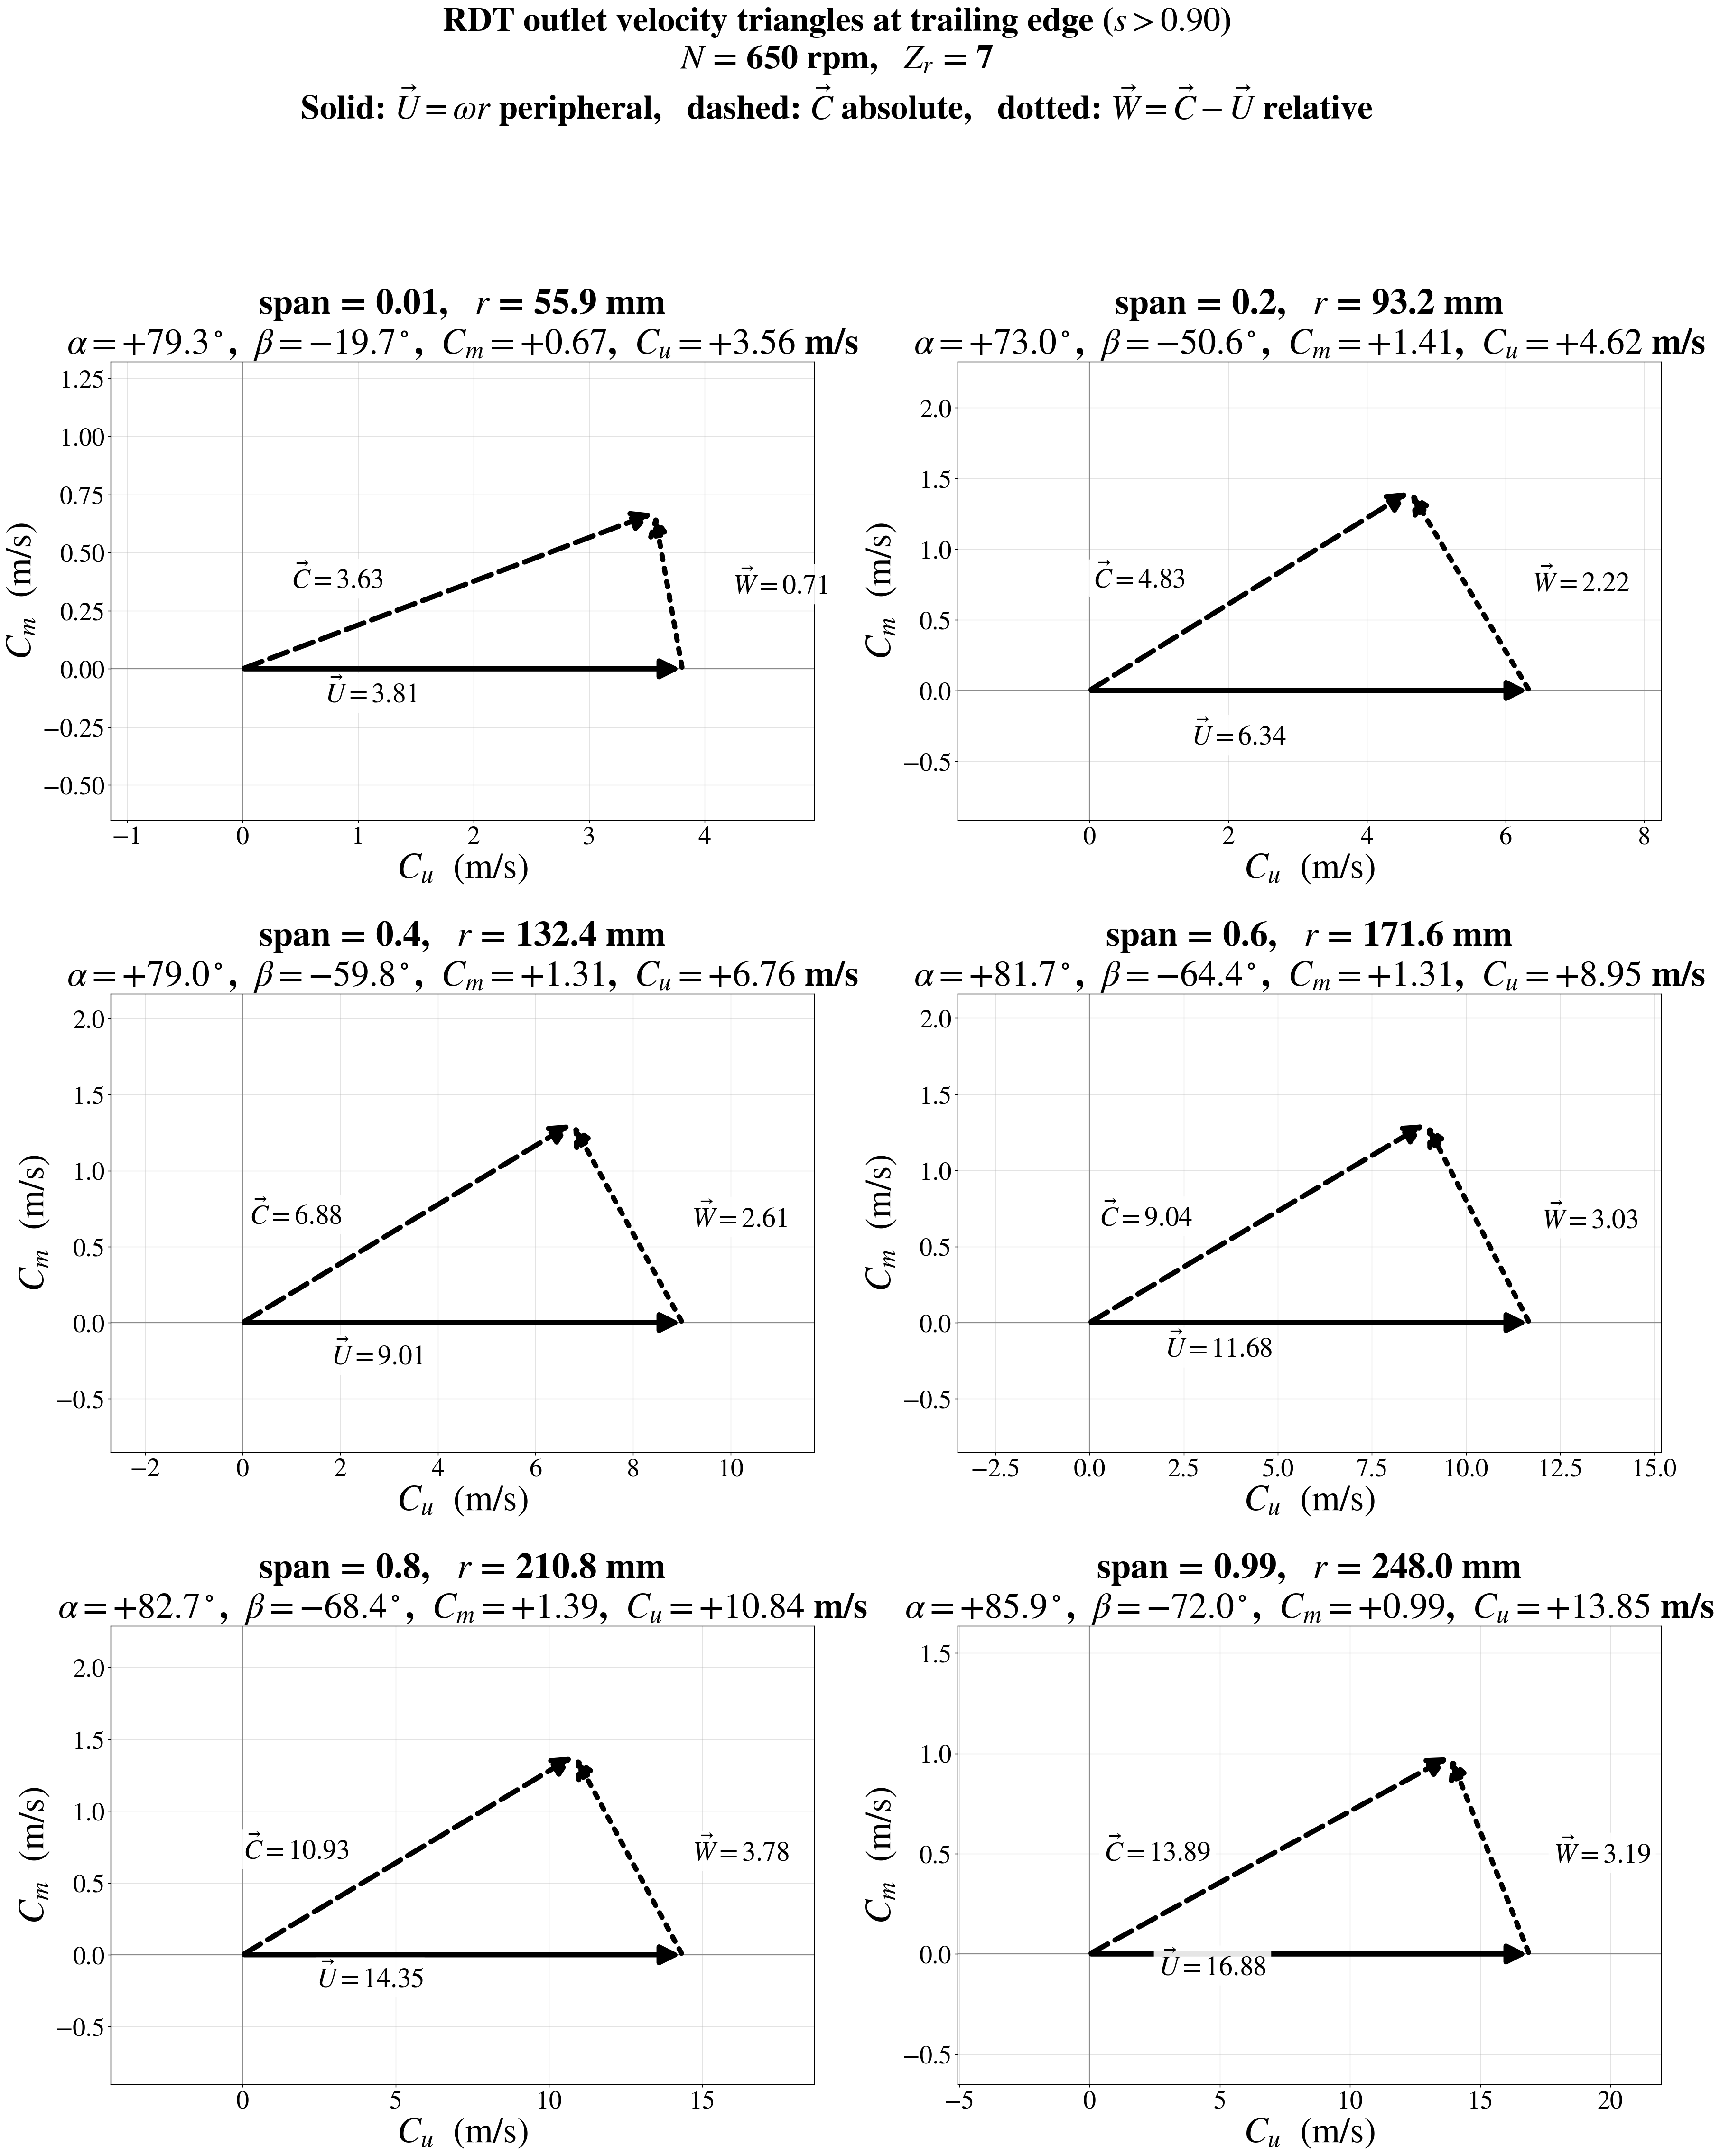
\includegraphics[width=0.99\linewidth]{Figures/RDT/RDT_velocity_triangles_TE.png}
  \caption[Velocity triangles at the RDT trailing edge]{Velocity triangles at the RDT trailing edge ($s>0.90$) for the six radial spans used to characterise the wake. Blue: absolute velocity $\vec{C}$; green: peripheral velocity $\vec{U}=\omega r$; red: relative velocity $\vec{W}=\vec{C}-\vec{U}$. The three vectors close as $\vec{C}=\vec{U}+\vec{W}$ by construction. Operating point: $N=650$~rpm, $Z_r=7$. Sign convention follows \eqref{eq:rdt_sign_convention}.}
  \label{fig:rdt_velocity_triangles_TE}
\end{figure}
 
\paragraph{Near-leading-edge values: complementary diagnostic.}
Figure~\ref{fig:rdt_velocity_triangles_LE} presents the velocity triangles constructed from the same blade-loading exports but evaluated in the near-LE window $s\in[0.05,\,0.15]$, after the LE stagnation/suction-peak spike has decayed and before the main chord-loaded region develops. Table~\ref{tab:rdt_le_values} summarises the corresponding components. These values describe the kinematic state of the flow on the rotor blade surface near the leading edge; they are \emph{not} the free-stream inlet velocity to the rotor. A free-stream inlet velocity would require a constant-$z$ plane export upstream of the rotor and is left to a follow-up post-processing step.
 
\begin{table}[H]
  \centering
  \caption[RDT near-LE velocity triangle at six spans]{Velocity-triangle components in the near-LE region ($s\in[0.05,\,0.15]$) of the RDT blade-loading lines. Reported as a complementary diagnostic of the kinematic state on the blade surface near the leading edge. These values are not used as guide-vane design input. Sign convention as in~\eqref{eq:rdt_sign_convention}.}
  \label{tab:rdt_le_values}
  \begin{tabular}{ccccccccc}
    \hline
    span & $r$ & $U$ & $C_m$ & $C_u$ & $W_u$ & $|\vec{C}|$ & $\alpha$ & $\beta$ \\
         & [mm] & [m/s] & [m/s] & [m/s] & [m/s] & [m/s] & [$^\circ$] & [$^\circ$] \\
    \hline
    0.01 &  55.9 &  3.81 & $-1.51$ &  6.63 & $+2.82$ &  6.80 & $+102.8$ & $+118.1$ \\
    0.20 &  93.2 &  6.34 &   0.37  &  4.80 & $-1.55$ &  4.81 &  $+85.6$ &  $-76.7$ \\
    0.40 & 132.4 &  9.01 &   1.40  &  4.88 & $-4.13$ &  5.08 &  $+74.0$ &  $-71.3$ \\
    0.60 & 171.6 & 11.68 &   2.23  &  6.27 & $-5.41$ &  6.66 &  $+70.5$ &  $-67.6$ \\
    0.80 & 210.8 & 14.35 &   1.84  &  8.30 & $-6.05$ &  8.50 &  $+77.5$ &  $-73.1$ \\
    0.99 & 248.0 & 16.88 &   0.16  & 10.88 & $-6.00$ & 10.89 &  $+89.2$ &  $-88.5$ \\
    \hline
  \end{tabular}
\end{table}
 
\begin{figure}[H]
  \centering
  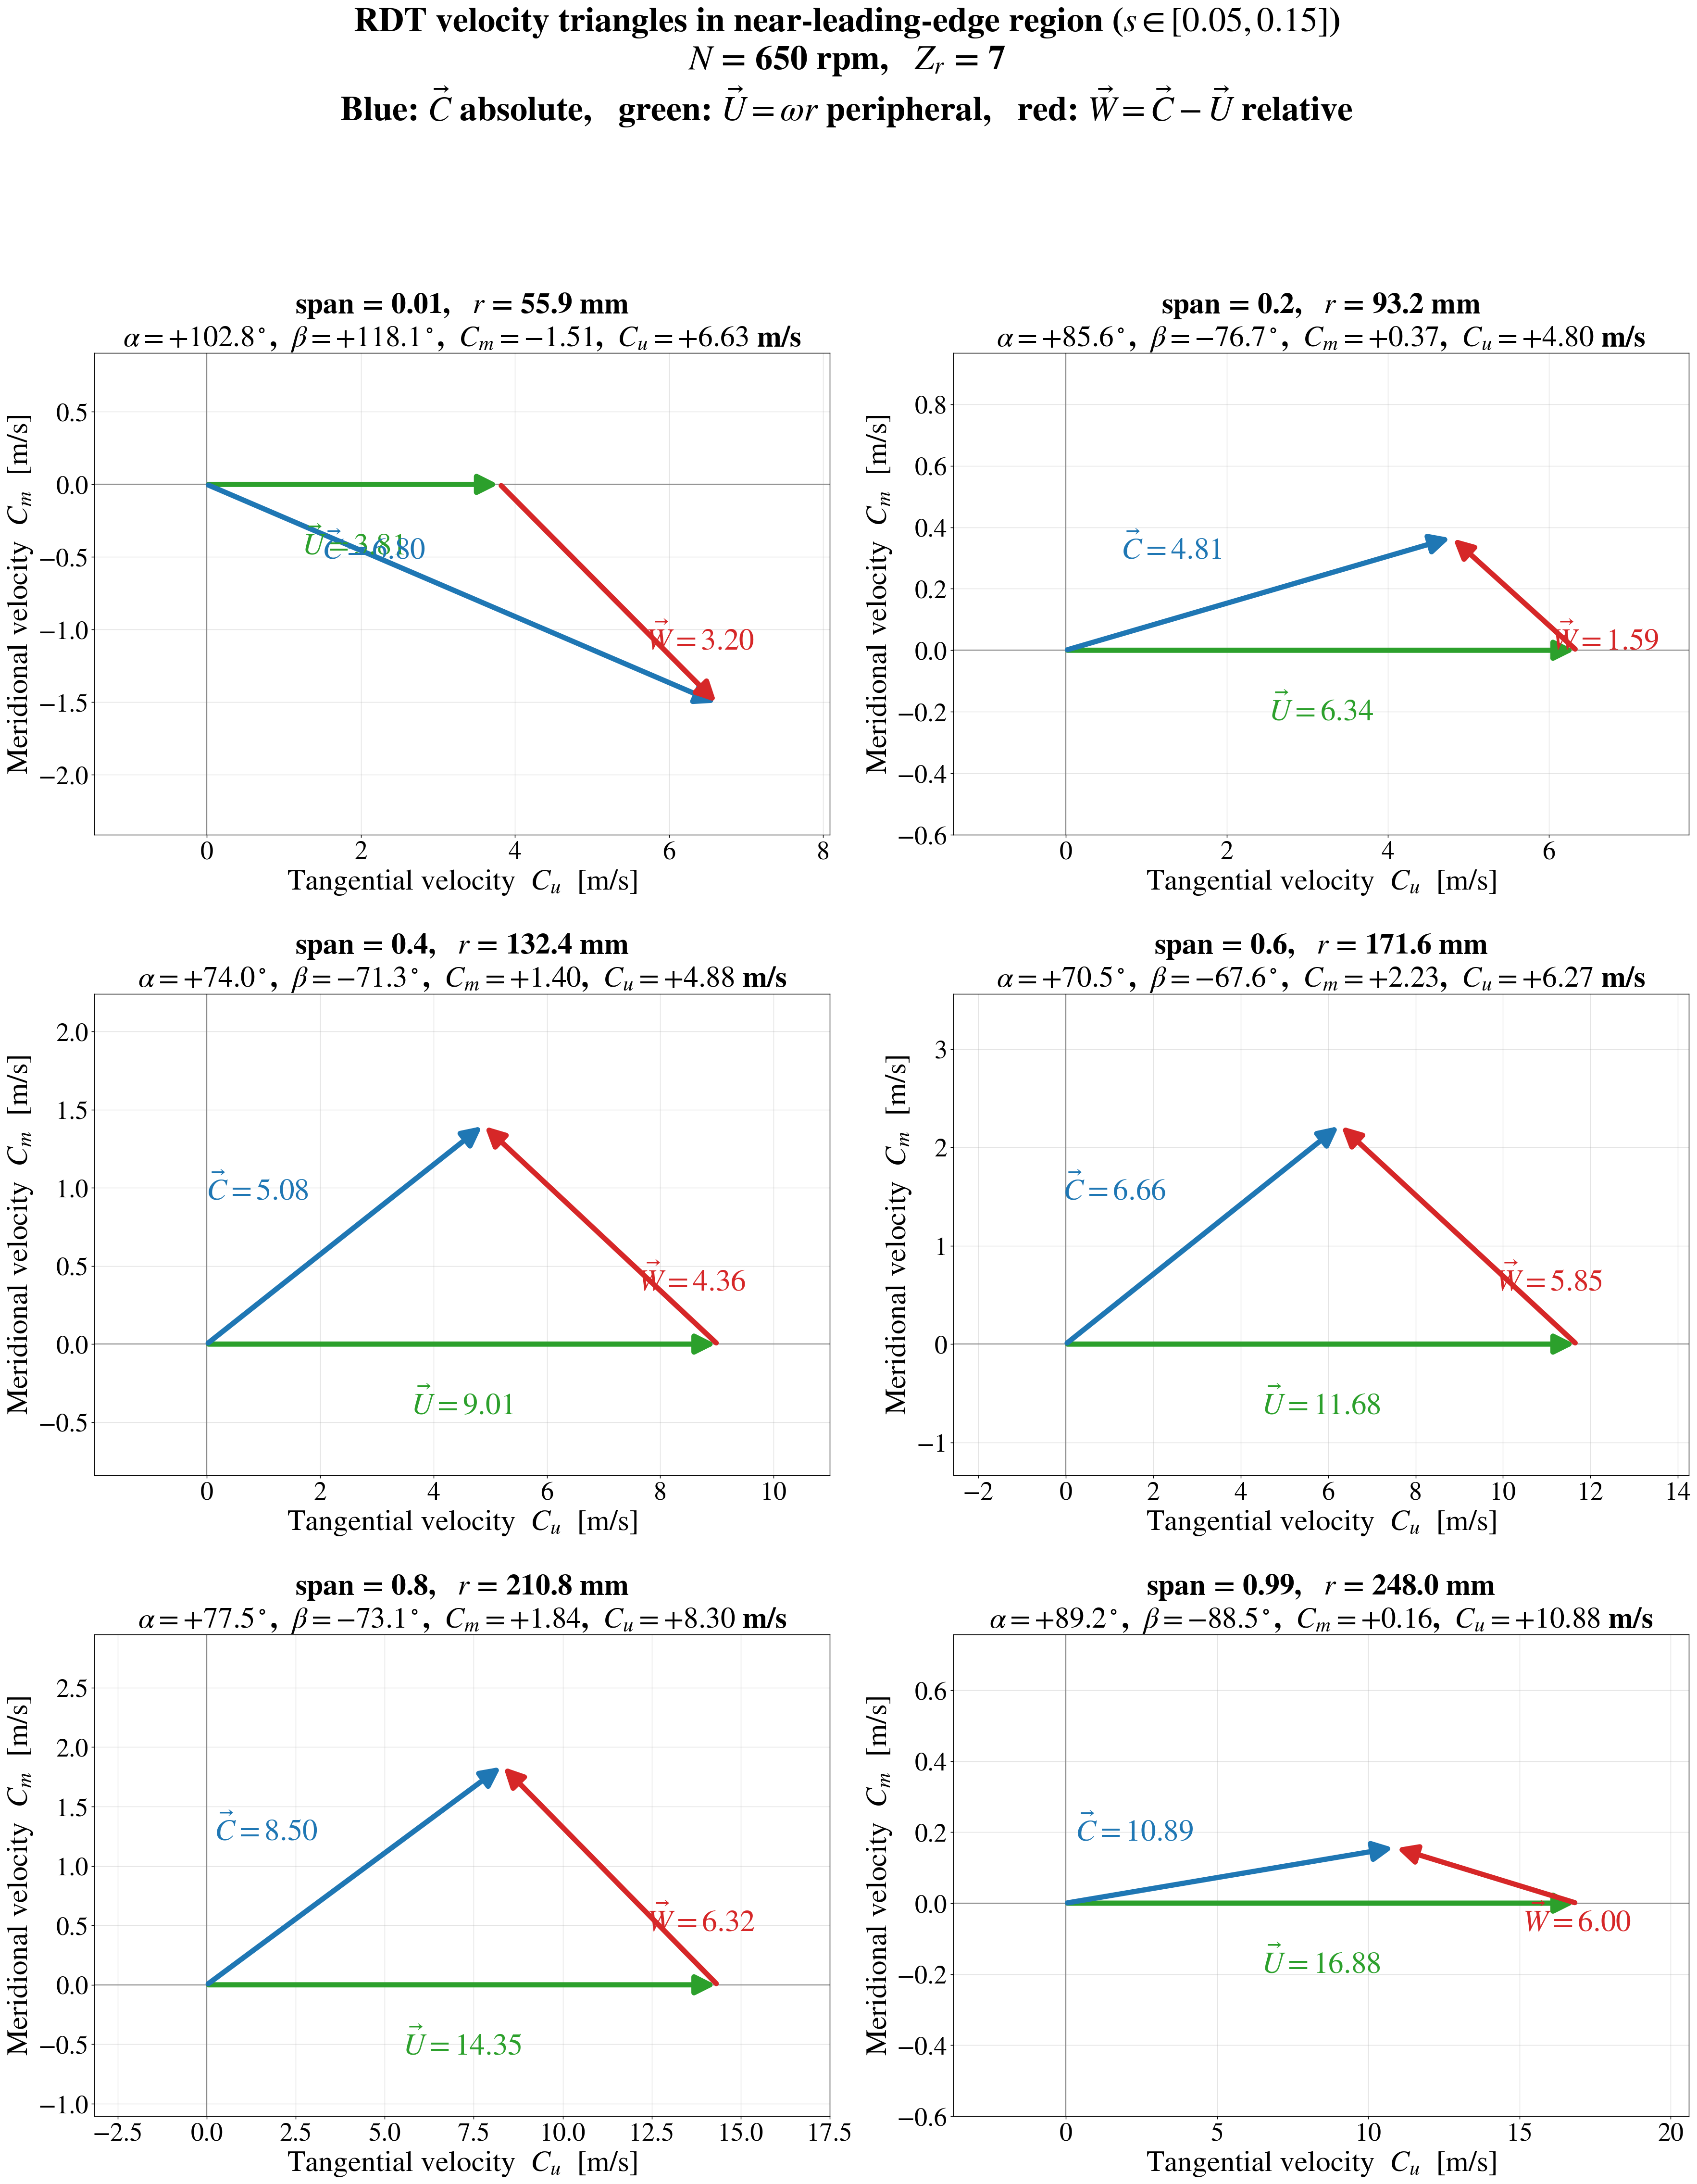
\includegraphics[width=0.99\linewidth]{Figures/RDT/RDT_velocity_triangles_LE.png}
  \caption[Velocity triangles in the near-LE region of the RDT]{Velocity triangles in the near-leading-edge region ($s\in[0.05,\,0.15]$) of the RDT blade-loading lines for the six radial spans. Same layout and vector convention as Figure~\ref{fig:rdt_velocity_triangles_TE}. The span-$0.01$ panel exhibits a negative $C_m$, reflecting the proximity of the LE stagnation/suction-peak structure on the blade surface near the hub rather than a physical reverse free-stream condition.}
  \label{fig:rdt_velocity_triangles_LE}
\end{figure}
 
\paragraph{Comparison of LE and TE regions.}
Comparing Tables~\ref{tab:rdt_te_values} and~\ref{tab:rdt_le_values} and Figures~\ref{fig:rdt_velocity_triangles_TE}-\ref{fig:rdt_velocity_triangles_LE} provides physical insight into how the rotor blade does work on the flow as it traverses the chord. Three points are worth noting.
 
First, the tangential component $C_u$ in the central span band ($r/R\in[0.40,\,0.80]$) is roughly $30$-$40\,\%$ smaller in the near-LE region than in the TE region. Examples: $4.88$~m/s vs.\ $6.76$~m/s at $r/R=0.40$, and $8.30$~m/s vs.\ $10.84$~m/s at $r/R=0.80$. This reflects the blade adding tangential momentum to the flow as it passes from LE to TE, consistent with the forced-vortex design intent of the upstream RDT~\cite{DjupeslandTrivedi2025}. The relative angle $\beta$ approaches $-90^\circ$ at the shroud in both regions, indicating that the relative flow there is nearly aligned with the negative tangential direction.

\clearpage